% concatenated from main.tex, commands.tex, figures/bad-group.tex, figures/visibility-proof.tex, figures/annulus-retraction.tex
\documentclass[11pt,a4paper]{amsart}
\usepackage[utf8]{inputenc}
\usepackage[T1]{fontenc}
% \usepackage{ntheorem}

% \usepackage[foot]{amsaddr}

\pdfoutput=1

\title{Almost planar finitely presented groups}

\author{John M. Mackay}
\address{School of Mathematics, University of Bristol, Bristol, BS8 1UG, UK.}
\email{john.mackay@bristol.ac.uk}
\author{Joseph P. MacManus}
\address{School of Mathematics,  University of Bristol, Bristol, BS8 1UG, UK, and the Heilbronn Institute for Mathematical Research, Bristol, UK.}
\email{joseph.macmanus@bristol.ac.uk}
\author{Davide Spriano}
\address{Mathematical Institute, University of Warwick, Coventry, CV4 7AL, UK.}
\email{davide.spriano@warwick.ac.uk}
\date{4th May, 2026}% Make sure to change to fixed date before submission



% uncomment to change margins
% \usepackage[a4paper,margin=1.35in]{geometry}

\usepackage{amsfonts}
\usepackage{amsmath}
\usepackage{amsthm}
\usepackage{amssymb}


\usepackage[abbrev,alphabetic]{amsrefs}
\usepackage{stmaryrd}
\usepackage{mathrsfs}  
\usepackage{todonotes}
\usepackage{graphicx}
\usepackage{tikz}
\usepackage{quiver}
% \usepackage{tgpagella}
\usepackage[colorlinks]{hyperref} % should usually be imported last
\hypersetup{
    % colorlinks=true,
    linkcolor=blue,
    citecolor=red,
}
% \usepackage{fancyref}
\usepackage{todonotes}
\usepackage{thmtools,thm-restate}
% \usepackage{showkeys}
%count sections from 0
% \setcounter{section}{-1}


%%%% Symbols %%%%
\DeclareMathOperator{\Cay}{Cay}
\DeclareMathOperator{\diam}{diam}
\DeclareMathOperator{\length}{length}
\DeclareMathOperator{\cut}{cut}
\DeclareMathOperator{\Ends}{Ends}
\DeclareMathOperator{\QI}{QI}
\DeclareMathOperator{\dHaus}{Haus}
\DeclareMathOperator{\dist}{d}
\DeclareMathOperator{\Aut}{Aut}
\DeclareMathOperator{\width}{width}
\DeclareMathOperator{\rank}{rank}
\DeclareMathOperator{\Homeo}{Homeo}
\DeclareMathOperator{\Hom}{Hom}
\DeclareMathOperator{\Con}{Con}
\newcommand{\bdry}{\partial_\infty}


% Sets
\newcommand{\R}{\mathbb{R}}
\newcommand{\bbH}{\mathbb{H}}
\newcommand{\Z}{\mathbb{Z}}
\newcommand{\N}{\mathbb{N}}
\newcommand{\Q}{\mathbb{Q}}
\newcommand{\C}{\mathbb{C}}

% Arrows
\newcommand{\into}{\hookrightarrow}
\newcommand{\onto}{\twoheadrightarrow}
\newcommand{\actson}{\curvearrowright}

% Group presentations
\newcommand{\pres}[2]{\langle #1 \ ; \ #2 \rangle}

% Todo notes
\newcommand{\joe}[1]{\todo[color=yellow]{\scriptsize{Joe: #1}}}
\newcommand{\davide}[1]{\todo[color=cyan]{\scriptsize{Davide: #1}}}
\newcommand{\john}[1]{\todo{\scriptsize{John: #1}}}



% referencing non-numbered list items

\makeatletter
\newcommand{\myitem}[1]{%
\item[#1]\protected@edef\@currentlabel{#1}%
}
\makeatother

%%%%%%%%%%%%%%%%%%%%%%%%%%%%%%%%%%%%%%%%%%%%%%%%%%%%%%%%%%%%%%%%%%%%%%%%%%%%%%%%

%%%% Theorem styles %%%%

\newtheorem{theorem}{Theorem}[section]% theorem counter resets every \subsection
% \renewcommand{\thetheorem}{\arabic{theorem}}% Remove subsection from theorem counter representation
\newtheorem{alphtheorem}{Theorem}
\renewcommand*{\thealphtheorem}{\Alph{alphtheorem}}

\newtheorem{alphcor}[alphtheorem]{Corollary}
% \renewcommand*{\thealphcor}{\Alph{alphcor}}
\newtheorem*{theorem*}{Theorem}

% italicised
\newtheorem{proposition}[theorem]{Proposition}
\newtheorem{lemma}[theorem]{Lemma}
\newtheorem{corollary}[theorem]{Corollary}
\newtheorem{claim}[theorem]{Claim}
\newtheorem{subclaim}[theorem]{Subclaim}
\newtheorem{question}[theorem]{Question}
\newtheorem{conjecture}[theorem]{Conjecture}

% non-italicised
\theoremstyle{definition}
\newtheorem{definition}[theorem]{Definition}
\newtheorem{example}[theorem]{Example}
\newtheorem{remark}[theorem]{Remark}

\newcommand{\dme}{\mathfrak{dme}}

\newcommand{\tw}{\mathrm{tw}}
\newcommand{\sn}{\mathrm{sn}}





%%%%%%%%%%%%%%%%%%%%%%%%%%%%%%%%%%%%%%%%%%%%%%%%%%%%%%%%%%%%%%%%%%%%%%%%%%%%%%%

\begin{document}


\begin{abstract}
    We show that finitely presented groups which admit $k$-planar Cayley graphs contain finite-index subgroups with planar Cayley graphs.
	More generally, we answer a question of Georgakopoulos and Papasoglu in the special case of coarsely simply connected graphs: a $k$-planar, coarsely simply connected, connected, locally finite, quasi-transitive graph is quasi-isometric to a planar graph.
    
    % Along the way, we show that any $k$-planar, one-ended, connected, locally finite, quasi-transitive graph is either quasi-isometric to the Euclidean plane, or maps regularly into the hyperbolic plane.

    % In this note we present substantial progress on this conjecture for one-ended graphs. In particular, we show that such a graph is either quasi-isometric to the Euclidean plane, or admits a regular map into the hyperbolic plane. We apply this observation, together with other technical results, to settle the aforementioned conjecture for Cayley graphs of a broad spectrum of groups, including hyperbolic and CAT(0) groups.
\end{abstract}

\maketitle




% \newpage

% \tableofcontents

% \newpage


\section{Introduction}

The study and classification of \textit{planar groups}---that is, finitely generated groups which admit planar Cayley graphs---is among the most classical topics in (geometric) group theory, beginning with Maschke's classification of the finite planar groups in 1896 \cite{maschke1896representation}. Infinite planar groups were classified much later, first by work of Wilkie \cite{wilkie1966non} and Zieschang--Vogt--Coldewey \cite{zieschang1970flachen} in the one-ended case. The multi-ended planar groups are more delicate, first studied by Droms \cite{droms2006infinite} and later enumerated by Georgakopoulos--Hamann \cite{georgakopoulos2019planari, georgakopoulos2023planar}, completing their classification.

As is typical in geometric group theory, it is often productive to consider properties `up to finite-index'. A finitely generated group is called \emph{virtually planar} if it contains a finite-index planar subgroup. While planar groups are tricky to classify on-the-nose, the class of virtually planar groups admits an easy and well-known description, as precisely those groups which are virtually free products of free and surface groups. Here, the interesting problem is not to classify these groups but to \emph{characterise} them via their geometry. More generally, one can ask the same about locally finite, quasi-transitive graphs which are quasi-isometric to planar graphs; note that every such graph is quasi-isometric to a planar group \cite{macmanus2024note}, and so morally we should expect such graphs to have analogous characterisations.
% commensurable to one of
% \begin{equation}\tag{$\diamondsuit$}\label{eq:v-planar-classes}
%     \{1\}, \ \ \ \Z, \ \ \ F_2, \ \ \ \Z^2, \  \ \  \pi_1\Sigma,  \  \ \ \Z \ast \Z^2, \ \ \ \Z \ast \pi_1\Sigma, \ \ \ \pi_1\Sigma \ast \Z^2,
% \end{equation}
% where $\Sigma$ denotes the closed orientable surface of genus two.

% \todo{John: I like this, here's a variation to consider, almost gets Theorem A on page 1!}
In this paper we seek such a characterisation by studying locally finite, quasi-transitive graphs which satisfy a weaker planarity hypothesis. 
Recall that a graph $\Gamma$ is said to be \emph{$k$-planar} if $\Gamma$ can be drawn in the plane so that each edge crosses at most $k$ other edges. The study of such graphs has its roots in work of Ringel \cite{ringel1965sechsfarbenproblem}, where attention was restricted to 1-planar graphs. The topic of $k$-planarity for $k > 1$ received attention from graph theorists much later, for the first time in work of Pach and T\"oth in 1997 \cite{pach1997graphs}.
The class of $k$-planar graphs is famously quite fickle. For example, the problem of deciding whether a given finite graph is even 1-planar is $\mathrm{NP}$-complete \cite{grigoriev2007algorithms}. This is in stark contrast to deciding planarity, which is solvable in linear time \cite{hopcroft1974efficient}. 

We will call  a graph \emph{almost planar} if it is $k$-planar for some $k \geq 0$. 
In the context of groups, almost planarity was first considered by Benjamini and Schramm in 1996 \cite{benjamini1996harmonic}.  Among other things, they show that almost planarity is a quasi-isometry invariant amongst bounded-degree graphs, and so it makes sense to speak of an \emph{almost planar group}, meaning a finitely generated group such that some/every Cayley graph of this group is an almost planar graph.  
The study of almost planarity in graphs and groups has appeared implicitly in the literature in many forms for quite some time. We give a brief survey of this below in Section~\ref{sec:intro-obsrtuctions}. 

The following conjecture, which has, on occasion, been referred to as the \emph{$k$-planar conjecture}, is of interest. It was posed by Georgakopoulos and Papasoglu {\cite[Prob.~9.4]{georgakopoulos2025graph}}; see also \cite[Conj.~6.1]{Esperet_Giocanti_2024}.

\begin{conjecture}[The $k$-planar conjecture]\label{conj:k-planar-conjecture}
    Let $\Gamma$ be a connected, locally finite, quasi-transitive
    graph. Then $\Gamma$ is almost planar if and only if it is quasi-isometric to some planar graph. 
\end{conjecture}


The `if' direction of Conjecture~\ref{conj:k-planar-conjecture} follows from the fact that almost planarity is a quasi-isometry invariant amongst bounded degree graphs. The converse poses an interesting challenge. 
% 
% 
The purpose of this article is to settle this conjecture for a large class of quasi-transitive graphs, namely those graphs which are \emph{coarsely simply connected}. See Definition~\ref{def:csc} for a precise definition of this property.

\begin{restatable}{alphtheorem}{mainresult}\label{thm:main-result}
Let $\Gamma$ be a connected, locally finite, quasi-transitive, coarsely simply connected 
    graph. Then $\Gamma$ is almost planar if and only if it is quasi-isometric to some planar graph. 
\end{restatable}

Most notably, the class of  connected, locally finite, quasi-transitive, coarsely simply connected 
    graphs includes Cayley graphs of finitely presented groups. In particular, we deduce the following corollary.

\begin{restatable}{alphcor}{maincorollary}\label{cor:intro-fpgroups}
    A finitely presented group is almost planar if and only if it is virtually planar.
\end{restatable}

The jump from `quasi-isometric to a planar graph' to `virtually planar' in the above follows from results in \cite{macmanus2023accessibility}, though it is also possible to prove this more directly using our intermediate results in this paper. We give such a direct proof in Section~\ref{sec:upgrade-to-qi} below.

Another source of examples comes from hyperbolic graphs, which are always coarsely simply connected \cite[{Prop.~$\Gamma$.3.23}]{bridson2013metric}.


\begin{restatable}{alphcor}{hypcorollary}\label{cor:intro-hypgroups}
    Every almost planar, hyperbolic, connected, locally finite, quasi-transitive graph is quasi-isometric to a planar graph.
\end{restatable}


% \todo{John: end of variation.  The paragraph "The class of virtually planar..." is nice, not sure where to put it.}

Our results add to the ever-growing list of characterisations of virtually planar groups, which is known to be a particularly rigid class of groups. Most famously, it is a deep theorem, originating in the work of Mess \cite{mess1988seifert} and completed with the convergence group theorem of Tukia, Gabai, and Casson--Jungreis \cite{tukia1988homeomorphic, gabai1992convergence, casson1994convergence}, that a finitely generated group which is quasi-isometric to a complete Riemannian plane is virtually planar. This was recently extended to the statement that any finitely generated group which is quasi-isometric to a planar graph (indeed, to a `string graph' \cite{davies2025string}) is virtually planar \cite{macmanus2023accessibility}. For finitely presented groups, this characterisation extends even further to groups which are `asymptotically minor-excluded'  \cite{macmanus2025fat}. 
See also \cite{bowditch2004planar, Esperet_Giocanti_2024, macmanus2025vertex, maillot2001quasi} for more entailments of this form.



The proof of Theorem~\ref{thm:main-result} is outlined in Section~\ref{sec:outline} below.  
Some of our intermediate results apply much more broadly, in turn settling Conjecture~\ref{conj:k-planar-conjecture} for many more graphs and groups. For example, we are able to prove the following statement for one-ended graphs. 

\begin{restatable}{alphtheorem}{mapintohypplane}\label{thm:intro-hyperbolic-plane}
    Let $\Gamma$ be a one-ended, connected, locally finite,  quasi-transitive graph. If $\Gamma$ is almost planar, then one of the following must hold:
    \begin{enumerate}
        \item $\Gamma$ is quasi-isometric to the Euclidean plane.

		\item $\Gamma$ admits a regular map into the hyperbolic plane.
    \end{enumerate}
\end{restatable}

A regular map is coarsely Lipschitz and bounded-to-one in a suitable sense, see Definitions~\ref{def:reg-map-graphs} and \ref{def:reg-map-spaces}.  
Note that a complete solution to Conjecture~\ref{conj:k-planar-conjecture} for one-ended graphs would require upgrading the regular map $f : \Gamma \to \mathbb H^2$ in Theorem~\ref{thm:intro-hyperbolic-plane} to be a quasi-isometry; indeed, even a coarse embedding would suffice: we find such an upgrade when $\Gamma$ is coarsely simply connected, see Section~\ref{sec:outline} below for discussion. 

We remark that Theorem~\ref{thm:intro-hyperbolic-plane} has the immediate consequence that a connected, locally finite, one-ended, almost planar, quasi-transitive graph is either quasi-isometric to the Euclidean plane or has logarithmic separation profile, in the sense of Benjamini--Schramm--Tim\'ar \cite{benjamini2012separation}. 
To the best of our knowledge, it is an open problem to exhibit a connected, locally finite, quasi-transitive graph with logarithmic separation profile which is not hyperbolic. We pose the existence of such a graph as a question below (Question~\ref{question:log-sep}). 

% Finally, we apply Theorem~\ref{thm:intro-hyperbolic-plane} in conjunction with another technical result---dubbed the \emph{flanking lemma} (\ref{lem:flanking-lemma})---to prove the following extension of Corollary~\ref{cor:intro-fpgroups}.
% 
% % \begin{alphtheorem}\label{thm:fp-subgroups}
% %     Let $G$ be a one-ended, finitely generated group, which contains a one-ended, finitely presented subgroup. If $G$ is almost planar then it is virtually planar.
% % \end{alphtheorem}
% 
% \begin{restatable}{alphtheorem}{fpsubgroups}\label{thm:fp-subgroups}
%     Let $G$ be a one-ended, finitely generated group, which contains a one-ended, finitely presented subgroup. If $G$ is almost planar then it is virtually planar.
% \end{restatable}
% 
% Note that there exist (necessarily one-ended) finitely generated, non-finitely presented groups where every subgroup is either cyclic or conjugate into a surface subgroup; see e.g. \cite[Thm.~L]{fournier2025dimensions}. In particular, Theorem~\ref{thm:fp-subgroups} does not follow na\"ively from Corollary~\ref{cor:intro-fpgroups} by simply passing to the given subgroup. 
% 
% We remark that Theorem~\ref{thm:fp-subgroups} is not the only application of the flanking lemma~(\ref{lem:flanking-lemma}), and serves more generally as a model argument which can be applied to (the 1-skeleton of) any one-ended, locally finite, cocompact 2-complex which contains a sufficiently rich family of disjoint, `thick', simply connected subcomplexes.

% In this paper we study Cayley graphs which satisfy a weaker planarity hypothesis. 
% Recall that a graph $\Gamma$ is said to be \emph{$k$-planar} if $\Gamma$ can be drawn in the plane so that each edge crosses at most $k$ other edges. We will call  $\Gamma$ \emph{almost planar} if there exists an integer $k \geq 0$ such that $\Gamma$ is $k$-planar. 
% In the context of groups, almost planarity was first considered by Benjamini and Schramm in 1996 \cite{benjamini1996harmonic}. Among other things, they show that a bounded-degree graph is almost planar if and only if it admits a regular map to some (bounded-degree) planar graph (see Theorem~\ref{prop:almost-planar-regular-map-char}). In particular,  almost planarity is a quasi-isometry invariant amongst bounded-degree graphs, and so it makes sense to speak of an \emph{almost planar group}, meaning a finitely generated group such that some/every Cayley graph of this group is an almost planar graph. 

% The study of almost planarity in graphs and groups has appeared implicitly in the literature in many forms for quite some time. We give a brief survey of this below in Section~\ref{sec:intro-obsrtuctions}. 
% The following conjecture was recently posed by Georgakopoulos and Papasoglu. 

% \begin{conjecture}\label{conj:k-planar-conjecture}
%     Let $\Gamma$ be a connected, locally finite, vertex-transitive
%     % \footnote{The original conjecture is stated for \emph{quasi-transitive} graphs. That is, graphs $X$ where $\Aut(X)$ acts cofinitely on $V(X)$. This generalisation is redundant, since every connected, locally finite, quasi-transitive graph is quasi-isometric to a connected, locally finite, vertex-transitive graph \cite[Prop.~5.1]{woess1994topological}. } 
%     graph. Then $\Gamma$ is almost planar if and only if it is quasi-isometric to some planar graph. 
% \end{conjecture}


% One direction of Conjecture~\ref{conj:k-planar-conjecture} is clear, since quasi-isometries are examples of regular maps. The converse poses an interesting challenge. We remark that if a connected, locally finite, vertex-transitive graph is quasi-isometric to a planar graph, then it is in fact quasi-isometric to one of the eight groups listed in (\ref{eq:v-planar-classes}) \cite{macmanus2024note}. 


% The main purpose of this article is to settle this conjecture for Cayley graphs of finitely presented groups.

% \begin{alphtheorem}\label{thm:main-result}
%     Every almost planar finitely presented group is virtually planar. 
% \end{alphtheorem}



\subsection{Known obstructions to almost planarity}\label{sec:intro-obsrtuctions}

We now walk through existing obstructions to almost planarity which appear (sometimes in disguise) in the literature to motivate our approach to this problem. We will not define most of the invariants mentioned and instead defer to references, unless they are directly relevant to this paper. 

One of the most straight-forward ways to obstruct almost planarity is through \emph{asymptotic dimension}. It is known that the asymptotic dimension of any planar graph (in fact, any graph excluding some finite minor) is at most two \cite{bonamy2023asymptotic} (see also \cite{fujiwara2021asymptotic, jorgensen2022geodesic}). Since asymptotic dimension is monotone with respect to regular maps \cite{benjamini2012separation}, we deduce that bounded-degree almost planar graphs have asymptotic dimension at most two.

Another powerful coarse invariant applicable here is the \emph{separation profile} $\mathrm{sep}_\Gamma(n)$ of a graph, introduced by Benjamini--Schramm--Tim\'ar in \cite{benjamini2012separation}. It is a consequence of the famous planar separator theorem of Lipton--Tarjan \cite{lipton1979separator} that a planar graph $\Gamma$ satisfies $\mathrm{sep}_\Gamma(n) = O(\sqrt n)$. If $f : \Gamma \to \Lambda$ is a regular map between bounded-degree graphs, it is known that $\mathrm{sep}_\Gamma(n) = O(\mathrm{sep}_\Lambda(n) )$. In particular, if the separation profile of a bounded-degree graph $\Gamma$ asymptotically dominates $\sqrt n$, then it cannot be almost planar. The separation profile has been computed for many classes of groups. This, in turn, settles Conjecture~\ref{conj:k-planar-conjecture} in many specific cases. For example, almost planar solvable groups must be virtually $\Z^2$ or virtually cyclic \cite{hume2020poincare, gournay2023separation} (in particular, virtually planar). This also implies that $BS(n, m)$ is not almost planar for all $|n| \neq |m|$ \cite{hume2022poincare}. Note that the separation profile \emph{doesn't} obstruct almost planarity for, say, $BS(2,2) \cong F_2 \times \Z$ or hyperbolic groups with conformal dimension less than two, both of which have separation profile $\lesssim \sqrt{n}$ \cite[Lem.~7.2]{benjamini1996harmonic}, \cite{hume2022poincare}.


Separation profiles are generalised by the family of invariants known as \emph{Poincar\'e profiles} $\Lambda_\Gamma^p(r)$, where $p$ ranges over $ [1,\infty)$. This recovers the separation profile via $\mathrm{sep}_\Gamma \simeq \Lambda_\Gamma^1$.  Spielman--Teng's bound on the eigenvalues of the Laplacian for bounded degree planar graphs implies the following, which we record as it is not explicitly in the literature.
\begin{theorem}\label{thm:planar-poincare-profile}
	For any planar graph $\Gamma$ of bounded degree, we have
        \begin{equation*}
                \Lambda_\Gamma^p(r) \lesssim
                \begin{cases}
                        \sqrt{r} & \text{ for } p \in [1,2], \text{ or } \\
                        r^{1-1/p} & \text{ for } p \in [2,\infty),
                \end{cases}
        \end{equation*}
	and this is sharp.
\end{theorem}
\begin{proof}
	The upper bound for $p=2$ is by Spielman--Teng~\cite[Thm.~3.3]{spielman-teng-07-spectral-planar}.
	The bound for $p < 2$ follows from~\cite[Prop.~5]{hume2020poincare}, and for $p >2$ from~\cite[Corollary 2.2]{hume-mackay-25-round-trees}.
 This is sharp when, for example, $X$ is given by attaching a $\mathbb{Z}^2$ quadrant and $3$-regular tree.
\end{proof}
Poincar\'e profiles are also monotone under regular maps, and have also been computed for certain classes of groups. For example, by \cite[Thm.~1.12]{hume2022poincare}, we have for $n > 1$ that $\Lambda_{F_n\times\mathbb{Z}}^2 (r) \simeq r^{2/3} \not\lesssim r^{1/2}$. In particular, this implies that $BS(n,\pm n)$ is almost planar if and only if $n = 1$, which settles Conjecture~\ref{conj:k-planar-conjecture} for Baumslag--Solitar groups. 
% We record this fact below for later reference. 

% \begin{proposition}\label{prop:bs-groups}
%     $BS(n,m)$ is almost planar if and only if $|n| = |m| = 1$. 
% \end{proposition}

In a completely different direction, we can also use the non-existence of certain harmonic functions to obstruct almost planarity. This is due to the work of Benjamini--Schramm. In \cite{benjamini1996harmonic}, they show that if $\Gamma$ is a transient, bounded-degree, connected, almost planar graph, then $\Gamma$ admits a non-constant bounded harmonic function with finite Dirichlet energy. This is a very powerful obstruction, ruling out almost planarity for a vast number of graphs (including $F_2 \times \Z$, see discussion before \cite[Lem.~7.2]{benjamini1996harmonic}). Most dramatically, it is a theorem of Medolla--Soardi that locally finite, quasi-transitive, amenable graphs do not admit such harmonic functions \cite[Thm.~5.2]{medolla1995extension}. Since non-transient locally finite quasi-transitive graphs are either finite or quasi-isometric to either $\Z$ or $\Z^2$ \cite[Thm.~5.13]{woess2000random}, this settles Conjecture~\ref{conj:k-planar-conjecture} for  amenable groups. 
This result also appears in another form in Woess' monograph; see \cite[p.~138]{woess2000random}. Furthermore, when combined with a theorem of Georgakopoulos \cite{georgakopoulos2010lamplighter}, this also implies that many wreath products are not almost planar; in particular the lamplighter group $\Z_2 \wr \Z$ is not almost planar. 

So where does this leave us? Consider the group given by the following presentation: 
$$
G = \pres{a,b,c,d,e,f}{[a,b]=[c,d]=[e,f]}.
$$
The presentation complex of $G$ is depicted in Figure~\ref{fig:bad-group}. 
\begin{figure}[h]
    \centering


\tikzset{every picture/.style={line width=0.75pt}} %set default line width to 0.75pt        

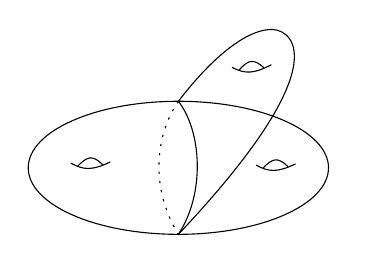
\begin{tikzpicture}[x=0.75pt,y=0.75pt,yscale=-1,xscale=1]
%uncomment if require: \path (0,300); %set diagram left start at 0, and has height of 300

%Shape: Ellipse [id:dp3290308398276839] 
\draw   (219.33,126.62) .. controls (219.33,108.91) and (251.72,94.56) .. (291.67,94.56) .. controls (331.62,94.56) and (364,108.91) .. (364,126.62) .. controls (364,144.32) and (331.62,158.67) .. (291.67,158.67) .. controls (251.72,158.67) and (219.33,144.32) .. (219.33,126.62) -- cycle ;
%Curve Lines [id:da6579209938829627] 
\draw    (291.67,94.56) .. controls (302.9,109.02) and (304.7,138.87) .. (291.67,158.67) ;
%Curve Lines [id:da5722117150821862] 
\draw  [dash pattern={on 0.84pt off 2.51pt}]  (291.67,94.56) .. controls (281.03,109.96) and (277.44,135.41) .. (291.67,158.67) ;
%Curve Lines [id:da4879550132904962] 
\draw    (291.67,94.56) .. controls (310.99,69.43) and (327.16,59.37) .. (337.34,60) .. controls (347.53,60.63) and (367.59,78.22) .. (291.67,158.67) ;
%Curve Lines [id:da22636631928444473] 
\draw    (336.48,76.93) .. controls (327.94,81.46) and (323.71,81.43) .. (317.49,78.23) ;
%Curve Lines [id:da028106302960074325] 
\draw    (332.91,78.41) .. controls (327.79,73.83) and (325.4,74.49) .. (320.8,79.63) ;
%Curve Lines [id:da699965787702804] 
\draw    (258.87,123.78) .. controls (250.18,127.98) and (245.95,127.79) .. (239.85,124.35) ;
%Curve Lines [id:da15565365952893007] 
\draw    (255.25,125.12) .. controls (250.3,120.35) and (247.88,120.92) .. (243.11,125.88) ;
%Curve Lines [id:da28376642510979966] 
\draw    (348.13,124.72) .. controls (339.43,128.92) and (335.2,128.73) .. (329.11,125.3) ;
%Curve Lines [id:da29363533952799836] 
\draw    (344.5,126.06) .. controls (339.55,121.29) and (337.14,121.86) .. (332.37,126.82) ;




\end{tikzpicture}

    \caption{}
    \label{fig:bad-group}
\end{figure}

This is a one-ended hyperbolic group which is not virtually Fuchsian. According to Conjecture~\ref{conj:k-planar-conjecture}, it should not be almost planar. However, it slips through the net of all existing obstructions described above; it has asymptotic dimension equal to 2, its Poincar\'e profiles all satisfy the bound of Theorem~\ref{thm:planar-poincare-profile} \cite[Thm.~1.17]{hume-mackay-25-round-trees}, and it admits a non-constant bounded harmonic function with finite Dirichlet energy (as does every non-elementary hyperbolic group \cite{ancona2007positive}). 
It is this particularly troublesome group which motivated the toolbox developed in this paper, and indeed it follows from Corollary~\ref{cor:intro-fpgroups} that this group is not almost planar. 






\subsection{Outline of the proof of Theorem~\ref{thm:main-result}}\label{sec:outline}

We now describe the key steps in the proof of our main result. 

The first step is to prove Theorem~\ref{thm:intro-hyperbolic-plane}. To do so, we begin with a regular map $\Gamma\to \Lambda$ where $\Lambda$ is a planar, one-ended, bounded degree graph, and $\Gamma$ is a one-ended, locally finite, quasi-transitive graph; using one-ended-ness and a theorem of Richter--Thomassen \cite{richter20023}, we may assume that the drawing of $\Lambda$ in the plane is VAP-free.\footnote{\emph{VAP-free} stands for \emph{vertex accumulation point-free}, meaning that the image of the vertex set of $\Lambda$ in the plane is discrete.}  We then fill in discs and half-planes in the complement of $\Lambda$ with disks and half-planes from the hyperbolic plane to get a planar complex $P$.  If $P$ is not hyperbolic, this will be seen by bi-Lipschitz embedded loops in $P$ which---having limited interaction with the hyperbolic balls and half-planes---can be pulled back to $\Gamma$ to find subsets whose isoperimetric properties imply (by the Varopoulos inequality) that $\Gamma$ has at most quadratic growth. In particular, this implies that either $\Gamma$ is quasi-isometric to the Euclidean plane, or $P$ is Gromov-hyperbolic. We go on to show that our plane $P$ is in fact quasi-isometric to the hyperbolic plane $\bbH^2$ (see Theorem~\ref{thm:planes-QI-to-hypplane}), which implies Theorem~\ref{thm:intro-hyperbolic-plane}. 

We then proceed with the proof of Theorem~\ref{thm:main-result}. 
Applying results of Hamann on accessible graphs \cite{hamann2018accessibility, hamann2025tree}, which are graph-theoretic generalisations of theorems of Dunwoody \cite{dunwoody1985accessibility} and Papasoglu--Whyte \cite{papasoglu2002quasi}, we immediately reduce to the case that $\Gamma$ is one-ended.
Using Theorem~\ref{thm:intro-hyperbolic-plane}, we obtain that each such graph is either quasi-isometric to the Euclidean plane, or it admits a regular map into the hyperbolic plane. Without loss of generality, we may assume we are in the latter case. To prove Theorem~\ref{thm:main-result}, we need to promote this regular map into the hyperbolic plane to be a quasi-isometry. 
Assuming coarse simply connectedness allows us to replace the graph $\Gamma$ with a 2-dimensional, simply connected, cocompact simplicial complex $X$ admitting a continuous regular map into $\mathbb{H}^2$. 

The core intuitive idea is that we want to map $X$ into $\mathbb{H}^2$ `avoiding folds', essentially meaning that we want to avoid something like the absolute value map $\mathbb{R} \to \mathbb{R}_{\geq 0}$. Morally, such folds are what makes general regular maps far from being quasi-isometries. If one was guaranteed that nothing of the sort would happen, it is believable that a `foldless' regular map $X \to \mathbb{H}^2$ must force $X$ to have a quite restricted geometry. 

Of course, our map $f\colon X\to\mathbb{H}^2$ might not be so well-behaved. Our strategy consists in substituting such map with an improved one. Specifically, there are two properties that we want our improved map to have. The first one is called \emph{width-visibility} (Definition~\ref{defn:widthvisible}), and morally asks for bounded-diameter preimages on a net. To obtain a width-visible map we argue that if the diameter of $f^{-1}(x)$ was not uniformly bounded, we can use transitivity and Arzel\'a--Ascoli to modify the map and reduce a certain notion of complexity. The second one takes inspiration from the methods of Bonk and Kleiner used in \cite{bonk2002rigidity}, and is the notion of \emph{stability} (Definition~\ref{defn:stability}). Roughly, we say that a map is \emph{stable} at a point $x \in X$ if every `modification' $f'$ of $f$ supported in some ball around $x$ still covers $f(x)$. In other words, it is impossible to `push' the image of $f$ so that its image no longer covers $f(x)$. A non-example is depicted in Figure~\ref{fig:stability}. Applying an asymptotic dimension argument together with the Arzel\`a--Ascoli theorem again, we are able to produce another new map which has stable points, and moreover is `very stable': every point is stable for every size of ball.  This latter notion can be interpreted as a strong notion of surjectivity.

We then finish the proof by arguing that a map that is both very stable and width-visible must be a quasi-isometry. In particular, our graph is actually quasi-isometric to $\bbH^2$, which concludes the proof of Theorem~\ref{thm:main-result}. 



\begin{figure}[ht]
		\begin{tikzpicture}
			\node[anchor=south west,inner sep=0] (image) at (0,0) {\includegraphics[width=0.8\textwidth]{figures/Stability.pdf}};
			\begin{scope}[x={(image.south east)},y={(image.north west)}]
				%\draw[help lines,xstep=.1,ystep=.1] (0,0) grid (1,1);
				%\foreach \x in {0,1,...,9} { \node [anchor=north] at (\x/10,0) {0.\x}; }
				%\foreach \y in {0,1,...,9} { \node [anchor=east] at (0,\y/10) {0.\y}; }
				\node at (0.18, 0.43) {$x$};
                \node at (0.5, 0.44) {$f(x)$};
                \node at (0.835, 0.45) {$f(x)$};
                \node at (0.07, 0.85) {$X$};
                 \node at (0.45, 0.85) {$f(X)$};
                 \node at (0.79, 0.85) {$f'(X)$};
			\end{scope}
    \end{tikzpicture}\caption{Folds create non-stability: the map $f$, which folds the plane onto itself, is not stable because there is a modification $f'$ that agrees with $f$ outside the red ball and that avoids $f(x)$.}\label{fig:stability}
	\end{figure}



\subsection{Questions}

We conclude this introduction by stating two existential questions. A negative answer to both of these questions would settle Conjecture~\ref{conj:k-planar-conjecture} in its entirety. 

Firstly, as was remarked above, Theorem~\ref{thm:intro-hyperbolic-plane} implies that any almost planar, one-ended, connected, locally finite, quasi-transitive graph $\Gamma$ is either quasi-isometric to the Euclidean plane (in which case, we are very happy), or it has logarithmic separation profile. Currently, all known examples of finitely generated groups with logarithmic separation profile are hyperbolic. Even then, the structure of hyperbolic groups with such a separation profile is quite restrained \cite{lazarovich2025hyperbolic,hume-mackay-25-round-trees}. It is not inconceivable that these could be the only examples; if so, this would settle Conjecture~\ref{conj:k-planar-conjecture} entirely in the one-ended case. We thus pose this as a question (cf. \cite[Question 1.5]{hume2020poorly}).


\begin{question}\label{question:log-sep}
    Does there exist a connected, locally finite, quasi-transitive graph with logarithmic separation profile which is not hyperbolic?
\end{question}

Of course, a positive answer would not be entirely surprising, as the world of non-finitely presented groups is full of paradoxical constructions. For example, it is known that there exists examples of finitely generated groups---in particular, examples of so-called \emph{lacunary hyperbolic groups}---whose separation profile grows arbitrarily slowly on an infinite subset of its domain (though may explode outside of this subset); see \cite[Thm.~1.4]{hume2020poorly}. 


There is also the issue of \emph{accessibility} to contend with. There are inaccessible groups which do not contain any one-ended subgroups (for example, see some of the groups constructed in \cite{dunwoody1993inaccessible}). Directly answering the following question is therefore imperative to settling Conjecture~\ref{conj:k-planar-conjecture}.


\begin{question}\label{question:inaccessible}
    Does there exist an inaccessible, connected, locally finite, quasi-transitive graph which is almost planar?
\end{question}

The fact that an inaccessible transitive graph cannot be quasi-isometric to a planar graph was the main technical result of \cite{macmanus2023accessibility}, and it is likely that resolution to Question~\ref{question:inaccessible} would involve reducing to this case. It is also known---a fact which is due to Esperet, Giocanti, and Legrand-Duchesne---that they cannot be minor-excluded \cite{esperet2024structure}. Outside of these results, our current understanding of the geometry of inaccessible transitive graphs is quite limited. 


\subsection*{Acknowledgements}

The first author would like to thank the Isaac Newton Institute for Mathematical Sciences, Cambridge, for support and hospitality during the programme ``Operators, Graphs, Groups'', where work on this paper was undertaken; this work was supported by EPSRC grant EP/Z000580/1.
He also thanks David Hume, Romain Tessera and, especially, Mario Bonk for discussions around Theorem~\ref{thm:planar-poincare-profile}.
The second author was supported by the Additional Funding Programme for Mathematical Sciences, delivered by EPSRC (EP/V521917/1) and the Heilbronn Institute for Mathematical Research. The third author was supported by a Royal Society University Research Fellowship  URF\textbackslash R1\textbackslash 251707, and he would like to thank Federico Vigolo for discussions on an early version of this paper.  
% We are grateful to Francesco Fournier-Facio for pointing us in the direction of the strange groups constructed in \cite{fournier2025dimensions}.


% \newpage



\section{Preliminaries}

In this section we establish our notational and terminological conventions.



% \subsection{Graphs and polygonal complexes}

% Throughout this paper, all graphs considered are simplicial, undirected, and unweighted. 
% Given a graph $\Gamma$, we denote by $V(\Gamma)$ its vertex and by $E(\Gamma)$ its edge set. 



\subsection{Coarse geometry}
In this paper we will often consider several metric spaces at the same time, to avoid confusion we will use subscripts to denote the metric space we are referring to. For instance, $\dist_X$ refers to the distance in the metric space $X$. The \emph{(closed) neighbourhood} of a set $A$ is the set $B_X(A, r)$ of points in $X$ at distance $r$ or less from $A$. We may sometimes suppress the decorative subscripts from our notation if the space under consideration is clear from context.

A map $f$ between metric spaces $X,Y$ is \emph{$(\kappa, \varepsilon)$--quasi-isometric embedding} if for any pair of points $x,y\in X$ it holds \[\frac{1}{\kappa} \dist_X (x,y) - \varepsilon \leq^{(1)} \dist_Y(f(x),f(y)) \leq^{(2)} \kappa \dist_X(x,y) + \varepsilon.\]
If only the inequality $(2)$ holds, we say that $f$ is \emph{$(\kappa, \varepsilon)$--coarsely Lipschitz}. A map is $\kappa$--bi-Lipschitz if it is a $(\kappa, 0)$--quasi-isometric embedding. 
A map is a \emph{$(\kappa, \varepsilon)$--quasi-isometry} if it is a $(\kappa, \varepsilon)$--quasi-isometric embedding and it is $\varepsilon$--coarsely surjective, meaning $B_Y(f(X), \varepsilon) = Y$. 



A metric space $X$ is said to have \emph{bounded geometry} if for all $r \geq 0$, there exists $n > 0$ such that every closed ball of radius $r$ in $X$ can be covered by $n$ balls of radius 1. Note that if $X$ is a graph, this is equivalent to asking that $X$ have bounded degree. 

The following definition will play a central role.

\begin{definition}[Coarsely simply connected]\label{def:csc}
    Let $\Gamma$ be a graph and $m\geq 3$ an integer. The \emph{$m$-filling} of $\Gamma$, denoted $X_m(\Gamma)$, is the polygonal 2-complex obtained by attaching 2-cells to all cycles of length at most $m$. 
    We say that  $\Gamma$ is \emph{coarsely simply connected} if there exists $m \geq 3$ such that $X_m(\Gamma)$ is simply connected.
\end{definition}

The motivating examples include Cayley graphs of finitely presented groups, as well as hyperbolic graphs.



\subsection{Regular maps}\label{ssec:reg-maps}

We now define the notion of a regular map. We will give two definitions, one for graphs and the other for generic metric spaces. 

\begin{definition}[Regular maps between graphs \cite{benjamini2012separation}]\label{def:reg-map-graphs}
    Let $\Gamma$, $\Lambda$ be graphs, and $\kappa \geq 1$ a constant. Then, a map $f : V(\Gamma) \to V(\Lambda)$ is said to be \emph{$\kappa$-regular} if the following hold:
\begin{enumerate}
    \item The map $f$ is $(\kappa,\kappa)$-coarsely Lipschitz. 
    \item For all $y \in V(\Lambda)$, we have that $|f^{-1}(y)| \leq \kappa$. 
\end{enumerate}
\end{definition}

We will often abuse notation and write $f : \Gamma \to \Lambda$, meaning $f : V(\Gamma) \to V(\Lambda)$. 


\begin{definition}[Regular maps between metric spaces {\cite[Def.~1.3]{benjamini1996harmonic}}]\label{def:reg-map-spaces}
    Let $X$, $Y$ be metric spaces. 
    Then, a map $f : X \to Y$ is said to be \emph{$\kappa$-regular} if the following hold:
\begin{enumerate}
    \item The map $f$ is $(\kappa,\kappa)$-coarsely Lipschitz. 
    \item For all $y \in Y$, we have that $f^{-1}(B_Y(y,1))$ can be covered by $\kappa$ balls of radius $1$. 
\end{enumerate}
\end{definition}

Note that we do not require $f$ to be continuous in the above definition. However, continuity will often be desirable, and so we may speak of \emph{continuous regular maps}. 

Regular maps arise naturally from subgraph inclusion, and from coarse embeddings (e.g.\ quasi-isometric embeddings) of graphs.  For example, if $G$ and $H$ are finitely generated groups and $H$ includes into $G$ as a subgroup, then this inclusion induces a regular map between the Cayley graphs of $G$ and $H$.



\subsection{Almost planar graphs and groups}\label{sec:prelims-almost-planar}


Recall that a graph is said to be \emph{$k$-planar} if it can be drawn in the plane such that every edge crosses at most $k$ other edges. For example, 0-planar graphs coincide with planar graphs. We say that a graph is \emph{almost planar} if it is $k$-planar for some finite $k \geq 0$. The minimal $k$ such that a graph is $k$-planar is sometimes called the \emph{local crossing number} of the graph.

The following is due to Benjamini and Schramm \cite{benjamini1996harmonic} (in fact, it is their original definition of almost planarity), and plays a central role throughout this paper. 


\begin{theorem}[{\cite[Thm.~1.8]{benjamini1996harmonic}}]\label{prop:almost-planar-regular-map-char}
    Let $\Gamma$ be a bounded-degree, connected graph. Then $\Gamma$ is almost planar if and only if there exists a planar, bounded-degree, connected graph $\Lambda$ and a regular map $\rho : \Gamma \to \Lambda$. 
\end{theorem}


This has the following immediate consequence. 

\begin{corollary}
    Let $\Gamma$, $\Lambda$ be connected, bounded degree graphs.
    If $f : \Gamma \to \Lambda$ is a regular map and $\Lambda$ is almost planar, then $\Gamma$ is almost planar.
\end{corollary}

In particular, almost planarity is a quasi-isometry invariant among connected graphs of bounded degree. This allows us to meaningfully describe a finitely generated group as an \emph{almost planar group}, meaning some/all of its Cayley graphs are almost planar graphs.
Then, another consequence of Theorem~\ref{prop:almost-planar-regular-map-char} is the following.

\begin{corollary}
    Let $G$ be a finitely generated group and $H \leq G$ a finitely generated subgroup. If $G$ is almost planar, then so is $H$.
\end{corollary}

\subsection{Hyperbolicity and boundaries}
We say that a geodesic metric space $X$ is \emph{$\delta$--hyperbolic} if for any geodesic triangle with sides $\alpha, \beta, \gamma$ the side $\gamma$ is contained in the $\delta$--neighbourhood of $\alpha\cup \beta$. A space is \emph{hyperbolic} if it is $\delta$--hyperbolic for some $\delta$. A group is hyperbolic if one (hence any) of its Cayley graphs with respect to a finite generating set is hyperbolic. 

For a hyperbolic space $X$, the \emph{Gromov boundary} $\partial_\infty X$ is the set of geodesic rays up to bounded Hausdorff distance. If $X$ is a space of bounded geometry, then $\partial_\infty X$ is a compact metrizable space. Given points $x, y, o \in X$, the \emph{Gromov product} $(x \mid y)_o$ is the quantity $\frac{1}{2}\left( \dist_X (o, x) + \dist_X(o, y) - \dist_X(x,y)\right)$. Given $a,b \in \bdry X$ we define \[ (a | b)_o = \sup \liminf_{t \to \infty} (\gamma(t)|\eta(t))_o \] where the supremum is over geodesic rays $\gamma, \eta$ based at $o$ representing $a,b$ respectively.  It is sometimes convenient to denote a geodesic ray from $o$ representing $a \in \bdry X$ as $[o,a)$.  A \emph{visual metric} is a metric $\rho$ on $\partial_\infty X$  such that there are $\varepsilon, C>0$ so that for any $a, b \in \partial_\infty X$ it holds $\frac{1}{C}e^{-\varepsilon (a \vert b)_o} \leq \rho(a, b) \leq C e^{\varepsilon (a \vert b)_o}$. The topology induced by any visual metric coincides with the Gromov topology. 


% \newpage


% \subsection{Separation profiles}

% Separation profiles tell us a lot about this conjecture, via the following corollary of the famous planar separator theorem. 

% \begin{proposition}
%     Let $G$ be a finitely generated group. If $sep_G(n)$ dominates $\sqrt n$, then $G$ is not almost planar.
% \end{proposition}


% \begin{corollary}
%     Given distinct $m, n > 0$, the group $BS(n,\pm m)$ is not almost planar. 
% \end{corollary}

% \begin{proof}
%     The separation profile of $G = BS(n,m)$ is given in \cite{hume2022poincare}, and is asymptotically $n / \log n$. This dominates $\sqrt n$. 
% \end{proof}

% \begin{corollary}
%     Groups of polynomial growth are almost planar if and only if they have quadratic growth.
% \end{corollary}

% \begin{proof}
%     If the growth is of degree $d$, the separation profile is  $\sim n^{\frac {d-1}d}$ \cite{hume2020poincare}. 
% \end{proof}

% Note that a group of quadratic growth is necessarily virtually $\Z^2$. 

% \begin{corollary}
%     Finitely generated solvable groups are almost planar if and only if they are virtually $\Z^2$.
% \end{corollary}

% \begin{proof}
%     This follows from \cite[Thm.~1.7]{gournay2023separation}, which says that solvable groups with separation bounded above by some power of $n$ are virtually nilpotent. 
% \end{proof}

% A related obstruction, which has not been explicitly recorded in the literature, is as follows.  Benjamini--Schramm--Tim\'ar introduced the ``separation profile'' $sep_X(r)$ of a graph $X$, and this was generalised to a family of ``Poincar\'e profiles'' $\Lambda_X^p(r), p \in [1,\infty)$, where $sep_X \simeq \Lambda_X^1$.  Spielman--Teng's bound on eigenvalues of the Laplacian for bounded degree planar graphs implies the following.
% \begin{theorem}[Spielman--Teng 2007, Hume--Mackay--Tessera]
%   For any planar graph $X$ of bounded degree,
%         \begin{equation*}
%                 \Lambda_X^p(r) \lesssim
%                 \begin{cases}
%                         \sqrt{r} & \text{ for } p \in [1,2], \text{ or } \\
%                         r^{1-1/p} & \text{ for } p \in [2,\infty).
%                 \end{cases}
%         \end{equation*}
% \end{theorem}
% This is sharp when, for example, $X$ is the union of a $\mathbb{Z}^2$ quadrant and $3$-regular tree (attached by an edge, say).
% This bound may apply to graphs where separation alone does not obstruct almost planarity, as in the following example.  (For this example, Benjamini--Schramm had already ruled out almost planarity by a different method, as described below.)
% \begin{corollary}
%     For $n>1$, the group $F_n \times \mathbb{Z}$ is not almost planar.
% \end{corollary}
% \begin{proof}
%     By [Hume--Mackay--Tessera] $\Lambda_{F_n\times\mathbb{Z}}^2 (r) \simeq r^{2/3} \not\lesssim r^{1/2}$.
% \end{proof}

% \subsection{Harmonic functions}

% The following theorem of Benjamini--Schramm \cite{benjamini1996harmonic} can also be used to obstruct almost-planarity. 

% \begin{theorem}[Benjamini--Schramm]\label{thm:benjamini-schramm}
%     Let $\Gamma$ be a transient, bounded-degree, connected, almost planar graph. Then $\Gamma$ admits a non-constant bounded harmonic function with finite Dirichlet energy. 
% \end{theorem}

% For example, this can be used to show that $F_2 \times \Z$ is not almost planar. 

% \begin{corollary}
%     For $n > 1$, the groups $F_n \times \Z$ and $BS(n,\pm n)$  are not almost planar. 
% \end{corollary}

% \begin{proof}
%     Let $C$ denote the infinite comb. That is, it is the graph obtained by deleting the horizontal edges in the 2-dimensional grid save for the $x$-axis. The graph $C \times \Z$ is transient (random walks diverge) \cite[Thm.~18.3]{woess2000random}, but (apparently) does not admit non-constant bounded harmonic functions \cite{benjamini2012separation} (they do not give a proof, but they probably know what they are talking about). This implies by Theorem~\ref{thm:benjamini-schramm} that this graph cannot be almost planar. 

%     This graph QI-embeds into the given groups, and so they too cannot be almost planar. 
% \end{proof}

% This, in turn, settles the main conjecture for RAAGs. 

% \begin{corollary}
%     We have that a RAAG is almost planar if and only if it is planar.
% \end{corollary}

% \begin{proof}
%     Every non-planar RAAG contains either $\Z^3$ or $F_2 \times \Z$ as a subgroup. 
% \end{proof}

% We can also say the following, very strong result.

% \begin{corollary}
%     Let $G$ be a one-ended amenable group. Then $G$ is almost planar if and only if it is virtually $\Z^2$.
% \end{corollary}

% \begin{proof}
%     By \cite[Thm.~5.2]{medolla1995extension}, $G$ does not admit non-constant bounded harmonic functions with finite Dirichlet energy. Moreover, $G$ is transient if and only if it does not have quadratic growth \cite{}.\todo{find a reference for this fact.} We are then done by Theorem~\ref{thm:benjamini-schramm}. 
% \end{proof}







% \subsection{Tree-width of balls}

% In a different direction, it is sometimes possible to attack this problem in specific instances using ideas from structural graph theory. 



% \begin{proposition}[\cite{robertson1984graph}]\label{prop:planar-diameter-tw}
%     Let $\Gamma$ be a finite connected graph of diameter $D$. Suppose $\Gamma$ is planar. Then the tree-width of $\Gamma$ is at most $3D+1$. 
% \end{proposition}

% It is not hard to extend this fact to the following. 

% \begin{lemma}\label{lem:k-planar-tw}
%     Let $\Gamma$ be a finite connected graph of diameter $D$. Suppose $\Gamma$ is $k$-planar. Then the tree-width of $\Gamma$ is at most $6(k+1)D+2$. 
% \end{lemma}

% \begin{proof}
%     Suppose $\Gamma$ is $k$-planar, given a drawing of $\Gamma$ realising this crossing number, we form a new planar graph $\overline \Gamma$ by subdividing each edge into $k+1$ edges, and simply viewing each `crossing' as a new vertex. The original vertices of $\Gamma$ shall be called `dead' vertices, and the new vertices inserted shall be called `alive'. 
%     Note that 
%     $$
%     \diam(\overline \Gamma) \leq (k+1)D.
%     $$
%     In particular, by Proposition~\ref{prop:planar-diameter-tw} we have $\tw(\overline \Gamma) \leq 3(k+1)D+ 1$. Let $(T, \overline {\mathcal V})$ be a tree decomposition of $\overline \Gamma$ realising this width, where, say, $\overline {\mathcal V} = (\overline B_t)_{t \in V(T)}$.  

%     Let us now form a tree decomposition of $\Gamma$. Consider $(T, \mathcal V)$, where $T$ is the same tree as in the given tree decomposition of $\overline \Gamma$, and $\mathcal V = (B_t)_{t \in V(T)}$ is defined as follows:

%     Fix an orientation of each edge in $\Gamma$. For each such (oriented) edge $e$ of $\Gamma$ with endpoints $u$ and $v$, let $v_0, \ldots, v_r$ denote the vertices along the corresponding path in $\overline \Gamma$, so that $u = v_0$, $v = v_r$, and $r \leq k+1$. We say that $v_1, \dots, v_{r-1}$ are the alive vertices \emph{associated with $e$}. Note that each alive vertex will be associated with exactly two edges in $\Gamma$. We also call $v_0$ the \emph{initial dead vertex} and $v_r$ the \emph{terminal dead vertex} associated with $e$. 
%     Given $t \in V(T)$, we modify $\overline B_t$ by removing every alive vertex $u$, say associated to the oriented $e_1$, $e_2$ of $\Gamma$, and add back the initial dead vertices associated to these edges. Repeating this for every alive vertex in $\overline B_t$, we call the resulting set $B_t$. 
    
%     It is clear that $|B_t|$ is at most twice the order of $|\overline B_t|$, since for every vertex removed we add at most two back. 
%     We need only check that $(T,\mathcal V)$, with $\mathcal V = (B_t)_{t\in V(T)}$, is a valid tree decomposition of $\Gamma$.
    
%     Firstly, it is clear that the $B_t$ cover $V(\Gamma)$. Secondly, let $u, v \in V(\Gamma)$ be adjacent. Let $e$ be the edge connecting them, assuming without loss of generality that $e$ is oriented such that $u$ is the initial vertex. Let $v_0, \ldots, v_r$ be the associated alive vertices. Then $u$ has been added to every bag that $v_{r-1}$ was part of. One of these bags contains $v = v_r$, since $(T, \overline {\mathcal V})$ was a valid tree decomposition. Thus, $u$ and $v$ are some common bag.
    
%     Finally, we need only check that the bags containing any particular $v \in V(\Gamma)$ induce a connected subtree of $T$. Now, we certainly have that 
%     $$
%     \{t \in V(T) : v \in \overline B_t\}
%     $$
%     induces a connected subtree of $T$, call this subtree $S_0$. Now, let $t_0 \in V(T)$ be such that $v \not\in \overline B_{t_0}$, but $v \in B_{t_0}$. Then there is some oriented edge $e$ in $\Gamma$ with associated vertices $v_0, \ldots, v_r$ in $\overline \Gamma$ ,  such that $v=v_0$ is the initial dead vertex of $e$, and some $v_i \in \overline B_t$ with $0 < i < r$. Given such an $i$, let $S_i$ be the subtree of $T$ spanned by $v_i$ in the tree decomposition $(T, \overline {\mathcal V})$. We have by construction that $v \in B_t$ for every $t \in V(S_i)$, $0 < i < r$. Also, $S_i \cap S_{i-1}$ is non-empty for every such $i$. This means that there is a path in $T$ from $t_0$ back to $S_0$, following only vertices $t$ such $v \in B_t$. It follows that $(T,\mathcal V)$ is a tree decomposition. 
% \end{proof}

% We make no claim that the above constant is tight. 



% \begin{theorem}\label{thm:tree-width-of-balls-obstructs}
%     Let $G$ be a finitely generated group with Cayley graph $\Gamma$. Let $W_r$ denote the tree-width of a ball of radius $r$ in $\Gamma$. If $W_r$ is superlinear in $r$, then $G$ is not almost planar. 
% \end{theorem}

% \begin{proof}
    
% \end{proof}

% One way of applying the above is to use the following device, which we call \emph{diametric minor efficiency}. 

% \begin{definition}[Diametric minor efficiency]
%         Let $\Gamma$ be a connected graph which is not minor-excluded. Given $n \in \N$, define
%         $$
%         \dme_\Gamma(n) := \min\{\diam_\Gamma(Y) : \text{$Y \subset \Gamma$ is a $K_n$-minor} \}. 
%         $$
% \end{definition}

% It is important to note that $\diam_\Gamma(Y)$ here denotes the diameter of $Y$ in the ambient metric of $\Gamma$, not with its own intrinsic metric. 

% \begin{corollary}
%     Let $\Gamma$ be a connected graph which is not minor-excluded. If $\dme_\Gamma(n)$ is sublinear, then $\Gamma$ is not almost planar.
% \end{corollary}





% \newpage


% \section{Almost planar Cayley complexes}


% We now turn our attention to the special case of finitely presented groups, and attempt to develop some general tools which could be helpful. 


% \subsection{Simplicial regular maps into planes}





% \begin{definition}
%     Let $K$, $L$ be simplicial complexes. Let $f : V(K) \to V(L)$ be a simplicial map. Then the \emph{simplicial width of $f$}, denoted $\width_\Delta(f)$, is defined as 
%     $$
%     \width_\Delta(f) = \sup\{\#(f^{-1}(v)) : v \in V(L)\}.
%     $$
%     The map $f$ is said to be a \emph{$\kappa$-regular simplicial map} if $\width_\Delta(f) \leq \kappa$.
% \end{definition}




% \begin{lemma}\label{lem:finite-components-in-fp2-groups}
%     Let $G$ be a one-ended, $FP_2$ group. Let $\Gamma$ be a connected graph upon which $G$ acts freely and cocompactly. Then, for all $n > 0$ there exists $m > 0$ such that the following holds:

%     Given any $S \subset V(\Gamma)$ with $\#(S) \leq n$, then any bounded connected component of $\Gamma - S$ contains at most $m$ vertices. \todo{This is true for all  finitely generated groups, by Varopoulos.}
% \end{lemma}

% \begin{proof}
%     Let $U \subset \Gamma - S$ be a bounded connected component. We will first bound the diameter of $\partial U$ by a constant $D = D(n, \Gamma) \geq 0$.

%     Since $G$ is $FP_2$, fix $r > 0$ such that the $r$-Rips complex $X = \mathrm{Rips}_r(\Gamma)$ satisfies 
%     $
%     H_1(X) = 0
%     $. 
%     Suppose $\diam_\Gamma(\partial U) > 10nr$. Then we can construct a non-trivial 1-cycle as follows...
%     [...]
%     This is a contradiction. Thus, setting $D = 10nr$, the claim follows.

%     Now, we have that $U$ must be contained in the $2D$-neighbourhood of $\partial U$, otherwise $\Gamma$ cannot be one-ended. Since $\Gamma$ is bounded-degree, say $\Delta(\Gamma) = k$, it follows that 
%     $$
%     \#(U) \leq n k^{2D}
%     $$
%     Setting $m = nk^{2D}$, we are done.
% \end{proof}

% \begin{lemma}\label{lem:seperating-two-sets}
%     Let $G$ be a one-ended, $FP_2$ group. Let $\Gamma$ be a connected graph upon which $G$ acts freely and cocompactly. Then, for all $n > 0$ there exists $m > 0$ such that the following holds:

%     Suppose we have subsets $S, U, W \subset V(\Gamma)$ such that $\#(S) \leq n$, and $S$ separates every $u \in U$ from every $w \in W$, then either $\#(U) \leq m$ or $\#(W) \leq m$.
% \end{lemma}

% \begin{proof}
%     Follows fairly immediately from Lemma~\ref{lem:finite-components-in-fp2-groups}.
% \end{proof}

% \begin{proposition}\label{prop:almost-planar-simplicial-map-char}
%     Let $G$ be a one-ended, $FP_2$ group. Let $K$ be a connected, locally finite, simplicial 2-complex upon which $G$ acts freely and cocompactly.
%     Suppose further that $G$ is almost planar. 
%     Then, there exists a uniform subdivision $K'$ of $K$, a simplicial 2-complex $P$ with $|P| \cong \R^2$ and a simplicial map $f : V(K) \to V(P)$ with finite simplicial width. 
% \end{proposition}

% \begin{proof}
%     Write $\Gamma = K^1$. 
%     By Proposition~\ref{prop:almost-planar-regular-map-char}, there is a surjective regular map $r : \Gamma \to \Pi$, where $\Pi$ is some bounded-degree, connected planar graph. Recall the definition of an \emph{almost 2-connected graph} from  \cite[Def.~1.18]{macmanus2023accessibility}
    
%     \begin{claim}
%         $\Pi$ is one-ended and almost 2-connected. 
%     \end{claim}

%     \begin{proof}
%         If not, get a pretty quick contradiction to the regularity of $r$.
%     \end{proof}

%     Using this, we may assume without loss of generality that $\Pi$ is 2-connected and one-ended. Since $r$ is regular (and thus Lipschitz), we may pass to uniform subdivisions of $\Gamma$ and $\Pi$ so that the map $r : \Gamma \to \Pi$ is simplicial. We may embed $\Pi$ into a triangulation of the plane $P$ in a standard way, with the $\Pi$ forming a QI-embedded subgraph of the 1-skeleton $P^1$.

%     After subdividing $\Gamma$, the complex $K$ has become a polygonal complex $K_1$ with 1-skeleton equal to $\Gamma$. We subdivide further the 2-cells of $K_1$ (without further subdividing $\Gamma$) so that the resulting complex $K_2$ is again simplicial, and so that we may extend the map $r : \Gamma \to \Pi$ to a simplicial map $f : K \to P$ in such a way that 
%     \begin{equation}\label{eq:boundary-property}
%         \partial f(\sigma) \subset f(\partial \sigma)
%     \end{equation}\todo{This needs elaboration. I also don't think it requires that the complex is simply connected, just cells of bounded size.}\todo{The point is that the interior regions bounded by the image of the loop can only contain so many vertices. Thus, to map the disk simplicially into these regions we need only take some uniform subdivision of it. The details of this should be worked out. The important point is that the interior of the disk is divided into boundedly many simplices/contains boundedly many interior vertices.}
%     for every one of the original 2-cells $\sigma$ of $K_1$. 
%     This concludes the definition of $f : K_2 \to P$. Note that the 1-skeleton of $K_1$ is still exactly $\Gamma$, and this in-turn includes as a subcomplex into $K_2$. 

%     We introduce some terminology. Vertices in $|K_2^0| \setminus |K_1^0|$ are called \emph{internal} vertices. Two internal vertices are said to be \emph{equivalent} if they lie inside the same 2-cell in $K_1$. Note that equivalence classes of internal vertices in $K_2$ under this relation naturally correspond to 2-cells of $K_1$.
    
%     We now need only check that preimages are of bounded size. This is equivalent to proving that only boundedly many non-equivalent internal vertices in $K_2$ map to a common vertex in $P$, since equivalence classes are uniformly bounded in size and boundedly many non-internal vertices lie in the preimage of any vertex in $P$ by the regularity of the map $r$. We also assume without loss of generality that $t$ (after passing to this subset) is odd, say $t = 2s+1$. 

%     Suppose then there exists $p \in |P^0|$ and a subset $\{v_1, \ldots, v_t\} \subset f^{-1}(p)$ of consisting of $t$ pairwise non-equivalent internal vertices, for some large $t > 0$. Let $\sigma_i$ denote the 2-cell of $K_1$ which contains $v_i$ within its interior.  
%     Let $c_i = \partial \sigma_i$. Since only boundedly many non-internal vertices can map to a common point in $P$, we may assume by taking $t$ large enough and passing to a subset that $f(c_i) \cap f(c_j) = \emptyset$ for $i \neq j$. 

%     By (\ref{eq:boundary-property}), we have that the $f(c_i)$ must be `nested' in $P$. That is, after possibly reordering, we may assume that $f(c_i)$ lies inside a bounded component of $|P|\setminus f(c_{i-1})$. In particular, $f^{-1}(c_{s+1})$ separates $c_{i}$ from $c_j$, for all $i \leq s$, $j \geq s+1$.
%     Let $A = f^{-1}(c_{s+1}) \cap \Gamma$. Then $A$ contains only boundedly many vertices, and has the property that it separates $c_{i}$ from $c_j$, for all $i \leq s$, $j > s+1$, inside of $\Gamma$. 
%     Applying Lemma~\ref{lem:seperating-two-sets}, this quickly puts a uniform bound on $s$ and thus $t$. The claim follows, and we are done.
% \end{proof}


% \newpage


\section{Proof of Theorem~\ref{thm:intro-hyperbolic-plane}}



In this section we prove Theorem~\ref{thm:intro-hyperbolic-plane} of the introduction. That is, if a one-ended, locally finite, quasi-transitive graph $\Gamma$ is almost planar, then either $\Gamma$ is quasi-isometric to $\R^2$, or maps regularly into $\bbH^2$. We prove this in several steps. 


\subsection{Gromov-hyperbolic planes}

We begin by observing that the hyperbolic plane is essentially the \emph{unique} visual, Gromov-hyperbolic, complete Riemannian plane, up to quasi-isometry.
% In this section we prove the following result, which characterises planes which are quasi-isometric to the hyperbolic plane.
First, we will need the following definition.

\begin{definition}[Visual space]
    Let $X$ be a geodesic metric space, $K \geq 0$. We say that $X$ is \emph{$K$-visual} if for every $x, y \in X$, there exists a geodesic ray $\gamma$ based at $x$ such that 
    $$
    \dist_X(y,\gamma) \leq K.
    $$
\end{definition}

We now prove the following.


\begin{theorem}\label{thm:planes-QI-to-hypplane}
    Let $P$ be a Gromov-hyperbolic, visual, complete Riemannian plane of bounded geometry. Then $P$ is quasi-isometric to the hyperbolic plane $\bbH^2$. 
\end{theorem}




\begin{proof}
	Let $\bdry P$ be the boundary at infinity of $P$ with some choice of visual metric $\rho$.
	
	We now assemble some results from the literature, omitting definitions which we do not work with directly.
	By Bonk--Schramm~\cite[Thms.~7.4,~8.2]{bonk2000embeddings}, $P$ is quasi-isometric to $\bbH^2$ if and only if $\bdry P$ and $\bdry \bbH^2 = \mathbb{S}^1$ are ``power quasisymmetric''.
	For connected metric spaces, being power quasisymmetric is equivalent to being quasisymmetric~\cite[Cor.~3.12]{TukiaVaisala-80-qs} (the ``$\lambda$-HD'' definition there is weaker than being connected).
	And again by Tukia--V\"ais\"al\"a~\cite[Thm.~4.9]{TukiaVaisala-80-qs}, a topological circle $Z$ is quasisymmetric to $\mathbb{S}^1$ if and only if it is ``HTB'' and ``BT''.  

	The ``HTB'' definition is equivalent to being ``doubling'', which holds for $\bdry P$ by the bounded geometry assumption~\cite[Thm. 9.2]{bonk2000embeddings}.

	The ``BT'' or ``bounded turning'' condition is also known as being ``linearly connected'': a metric space $Z$ is \emph{linearly connected} if there exists $L \geq 1$ so that for any $a,b \in Z$ there exists a connected set $J$ containing $a,b$ such that $\diam(J) \leq L \dist_Z(a,b)$.

	Summarising the discussion so far: to show $P$ is quasi-isometric to $\bbH^2$ it remains to show $\bdry P$ is a linearly connected topological circle.

	Moore showed that a topological space $Z$ is homeomorphic to $\mathbb{S}^1$ if and only if it is metrizable, connected, compact and has the property that for any distinct $x,y \in Z$, $Z \setminus \{x,y\}$ is disconnected (see e.g.~\cite[Thm.~2.28]{Hocking-Young-Topology}).

	Fix a basepoint $o\in P$ and hyperbolicity constant $\delta$ for $P$.
	Since $P$ is proper, $\bdry P$ is compact: any sequence of points $(a_i) \subset \bdry P$ has a convergent subsequence, since one can apply Arzel\`a--Ascoli to the sequence of geodesic rays $[o,a_i)$.

	We now see that $\bdry P$ is connected.  Assume the visual metric $\rho$ on $\bdry P$ satisfies 
	\[
		\frac{1}{C} e^{-\epsilon (a|b)_o} \leq \rho(a,b) \leq C e^{-\epsilon (a|b)_o}, \ \text{ for all } a,b \in \bdry P.
	\]
	For any large $R$ since $P$ is a Riemannian plane, there exists a topological circle $\gamma \subset P \setminus B(o,R)$ which disconnects $B(o,R)$ from infinity.
	For any $a,b \in \bdry P$, we can find geodesic rays $[o,a), [o,b)$ which hit $\gamma$ at some points $p,q$.  As $\gamma$ is connected, we can find a sequence of points $p=p_0, p_1,\ldots, p_n=q$ in $\gamma$ so that $\dist_P(p_{i-1},p_i) \leq 1$ for $i=1,\ldots,n$.  Since $P$ is visual, there exist geodesic rays $[o,a_i), i=0,\ldots,n$, going to points $a=a_0,a_1,\ldots,a_n=b$ in $\bdry P$, and so that $\dist_P(p_i,[o,a_i)) \leq K$.
	By hyperbolicity, $(a_i|a_{i+1})_o \geq \dist_P(o,p_i)-C' \geq R-C'$, where $C' = C'(\delta, K)$, and so $\rho(a_i,a_{i+1}) \leq C e^{-\epsilon (R-C')}$.
	Since $R$ was arbitrary, we conclude that $\bdry P$ is connected.

	We now show that removing any distinct $a,b \in \bdry P$ disconnects $\bdry P$.
	Since $P$ is proper and Gromov-hyperbolic, there exists a geodesic $\gamma:\R\to P$ so that $\gamma(-\infty)=a$ and $\gamma(+\infty)=b$.
	By the Jordan curve theorem, $\gamma$ disconnects $P$ into two components, $U$ and $U'$.
	For any $c \in \bdry P \setminus \{a,b\}$, any geodesic ray $[o,c)$, and any $C>0$, the set $B_P([o,c),C)\cap \gamma$ is bounded, else by hyperbolicity we would have $c=a$ or $c=b$.  In particular, which of $U$ or $U'$ the ray $[o,c)$ ends up in is independent of the choice of ray.

	Let $W,W' \subset \bdry P$ be the set of points $c \in \bdry P \setminus \{a,b\}$ for which the geodesic $[o,c)$ ends up in $U, U'$ respectively.
	By the above argument $\bdry P \setminus \{a,b\}$ is the disjoint union of $W$ and $W'$.
	Since $\gamma$ is a geodesic, $W$ and $W'$ are open because for each point of $W$ represented by $\xi$, a neighbourhood for $\xi$ contained in $W$ is obtained by considering all geodesics that diverge from $\xi$ after it last was $(2\delta+1)$-close to $\gamma$.
	Both $W$ and $W'$ are non-empty: choose $R$ much larger than $\delta$ and $\dist_P(o,\gamma)$.  Then the topological circle outside $B(o,R)$ contains points which are in both $U$ and $U'$, and a large (compared to hyperbolicity) distance from $\gamma$, so gives limit points in both $W$ and $W'$.
	So we have shown $\bdry P$ is a topological circle.  In fact, consequently we have seen that $W,W'$ are connected open intervals in $\bdry P$.

	It remains to show $\bdry P$ is linearly connected.
	Take $a,b \in \bdry P$, connected by a geodesic $\gamma \subset P$ at least say $10\delta$ from $o$ (else it suffices to bound the diameter of an arc connecting $a,b$ by $\diam(\bdry P)$).
	Suppose $U$ is the component of $P \setminus \gamma$ not containing $o$ and let $W$ be defined as before.
	Then $W \cup \{a,b\}$ is a connected set containing $a,b$, and any point $c \subset W$ is the limit of a geodesic ray which crosses $\gamma$, hence for suitable $C',C''$, $(a|c)_o \geq \dist_P(o,\gamma)-C' \geq (a|b)_o -C''$, thus for 
	\[
		\diam(W) \leq 2\sup_{c \in W} \rho(a,c) \leq 2e^{\epsilon C''}C^2 \rho(a,b). \qedhere
	\]
\end{proof}



\subsection{A criterion for visual-ness}

In order to apply Theorem~\ref{thm:planes-QI-to-hypplane}, we will need an easy way of establishing that a given Gromov-hyperbolic plane is visual. The following proposition provides such a criterion. 

\begin{lemma}\label{prop:criterion-for-visibility}
	Let $P$ be a $\delta$-hyperbolic, simplicial plane of bounded geometry. Suppose that there exists $C > 0$ such that every combinatorial Jordan curve of length at most $12\delta$ bounds a disk containing at most $C$ vertices. Then $P$ is visual. 
\end{lemma}

\begin{proof}
    We must show that there exists $K > 0$ such that for every $x, y \in P$, there exists a geodesic ray $\gamma$ based at $x$ such that $\dist_P(y,\gamma) < K$. 
    To do so, we will show that `balls are uniformly visual' and then apply the Arzel\`a--Ascoli theorem to conclude. 
    
	Let $r > C + 20 \delta$ and $x \in P$ be arbitrary. Let $S_r$ denote a simple closed curve in the 1-skeleton of $P$ such that 
    \begin{enumerate}
        \item the point $x$ lies in a bounded region of $P \setminus S_r$, and 

		\item for all vertices $s \in S_r$, we have that $\dist_P(s,x) = r$. 
    \end{enumerate}
	Such a simple closed curve $S_r$ certainly exists for any such $r\in\N$. 
    By the Jordan curve theorem, let $D_r$ denote the disk bound by $S_r$.  

    \begin{claim}\label{claim:spheres-are-visual}
        For all $y \in D_r$, there exists $z \in S_r$ and a geodesic $\gamma$ from $x$ to $z$ such that 
        $$
        \dist_P(y,\gamma) < C + 6\delta. 
        $$
    \end{claim}

    \begin{proof}
		For each vertex $z$ of $S_r$ choose once and for all a geodesic $\eta_z$ from $z$ to $x$ so that the choices form a tree, meaning that if $z,w\in S_r$ and $\eta_z(t) =\eta_w(t)$, then $\eta_z(s)  =\eta_w(s)$ for all $s\geq t$. In particular, either $y$ is already on one such geodesic, in which case we are done, or there exists a unique pair $z, w$ so that $y$ is in the interior of the triangle with sides $\eta_z, \eta_w$ and the edge $(z,w)$. Let $\Delta$ be the closure of such inside.  For $ n \leq \frac{r}{4\delta}$ define $z_n = \eta_z(n 4\delta)$, and define $w_n$ similarly (note that $\delta>0$). By hyperbolicity all triangles are uniformly $\delta$--thin. Thus we have $\dist_P(z_n, w_n) \leq  2\delta$ for all $n$. Additionally, for all $n$ choose once and for all a geodesic $[z_n, w_n]$ between $z_n, w_n$ that has connected intersection with both $\eta_z$ and $\eta_w$. The latter can be assumed by replacing the initial/final segment of $[z_n, w_n]$ with the appropriate segment of $\eta_z$/$\eta_w$. Moreover, for $n \neq m$ we must have $[z_n, w_n] \cap [z_m, w_m] = \emptyset$. If not, a triangular inequality argument would yield $\dist_P(z_n, z_m) < 4\delta$. A similar triangular inequality argument shows that $[z_n, w_n]$ cannot intersect the sphere of radius $ r- n4\delta + 2 \delta$ around $x$.    
        
    Intuitively, we want to use the geodesics $[z_n, w_n]$ to chop up  $\Delta$ in pieces of bounded perimeter, and conclude that $y$ must be contained in one such piece. For this, consider the quadrilaterals $Q_n$ with vertices $z_n, z_{n+1}, w_n, w_{n+1}$ and edges $[z_n, w_n], [z_{n+1},w_{n+1}]$ and the appropriate restrictions of $\eta_w, \eta_z$. If $Q_0$ contains $x$ then it must contain $\eta_z, \eta_w$ and the whole $\Delta$. So the claim is satisfied. So assume it is not the case. Consider $Q_1$. If $Q_1$ contains $y$, we are done. If $Q_1$ contains $x$, arguing as before we have that $Q_0 \cup Q_1$ contain the whole $\Delta$, and hence $Q_1$ contains $y$. If neither of the above happens, let $A_{n}$ denote complement of the ball $B_P(x, r-n4\delta)$. Since $[z_2, w_2]$ does not intersect the sphere of radius $r - 6\delta$ around $x$ we have 
    \[\Delta \cap  A_1 \subseteq Q_0 \cup Q_1.\]
    Proceeding inductively we have that for each $n$, either $y\in Q_n$ and we stop, or it must hold \[\Delta \cap A_n \subseteq \bigcup_{i =0}^n Q_i.\]
		If we don't stop, we eventually conclude $y \in B_P(x, 6\delta)$, and the hypothesis holds with $\gamma$ being any geodesic from $x$ to $S_r$. Otherwise, $y\in Q_n$ for some $n$. By construction, the perimeter of $Q_n$ is at most $12\delta$. Thus, the distance between $y$ and a point in $Q_n$ is at most $C$, otherwise $Q_n$ would contain a path containing more than $C$ vertices. Thus, the distance between $y$ and any point of $Q_n$ is at most $C+6\delta$. Since $Q_n$ contains points of the geodesic $\eta_w$, the claim follows for $\gamma = \eta_w$. See Figure~\ref{fig:visibility-proof} for a cartoon of this proof.
    \end{proof}

    \begin{figure}[h]
        \centering


\tikzset{every picture/.style={line width=0.75pt}} %set default line width to 0.75pt        

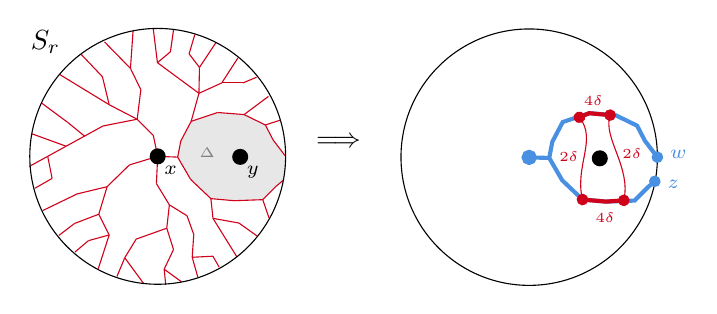
\begin{tikzpicture}[x=0.75pt,y=0.75pt,yscale=-1,xscale=1]
%uncomment if require: \path (0,300); %set diagram left start at 0, and has height of 300

%Shape: Polygon [id:ds5870025580965821] 
\draw  [draw opacity=0][fill={rgb, 255:red, 231; green, 231; blue, 231 }  ,fill opacity=1 ] (191.25,140.25) -- (192.75,132.5) -- (197.75,123) -- (210.5,118.75) -- (223.25,119.75) -- (233.5,124.75) -- (237.25,132) -- (243.25,139.88) -- (243.17,145.5) -- (242,151.5) -- (238.75,154.25) -- (232.25,160.75) -- (218.5,161.25) -- (207.25,160.25) -- (197.5,151) -- cycle ;
%Straight Lines [id:da7611547557085825] 
\draw [color={rgb, 255:red, 208; green, 2; blue, 27 }  ,draw opacity=1 ]   (168,144) -- (181.63,139.88) ;
%Straight Lines [id:da8633426985680359] 
\draw [color={rgb, 255:red, 208; green, 2; blue, 27 }  ,draw opacity=1 ]   (181.63,139.88) -- (179.5,129.75) ;
%Straight Lines [id:da6314254668219365] 
\draw [color={rgb, 255:red, 208; green, 2; blue, 27 }  ,draw opacity=1 ]   (191.25,140.25) -- (181.63,139.88) ;
%Straight Lines [id:da005799318879664561] 
\draw [color={rgb, 255:red, 208; green, 2; blue, 27 }  ,draw opacity=1 ]   (181,153) -- (181.63,139.88) ;
%Straight Lines [id:da6991596432469487] 
\draw    (181.63,139.88) ;
\draw [shift={(181.63,139.88)}, rotate = 0] [color={rgb, 255:red, 0; green, 0; blue, 0 }  ][fill={rgb, 255:red, 0; green, 0; blue, 0 }  ][line width=0.75]      (0, 0) circle [x radius= 3.35, y radius= 3.35]   ;
%Straight Lines [id:da692266463076252] 
\draw [color={rgb, 255:red, 208; green, 2; blue, 27 }  ,draw opacity=1 ]   (187.25,163.25) -- (181,153) ;
%Straight Lines [id:da39042446256274954] 
\draw [color={rgb, 255:red, 208; green, 2; blue, 27 }  ,draw opacity=1 ]   (186,174.5) -- (187.25,163.25) ;
%Straight Lines [id:da7276516459999517] 
\draw [color={rgb, 255:red, 208; green, 2; blue, 27 }  ,draw opacity=1 ]   (189.25,184.75) -- (186,174.5) ;
%Straight Lines [id:da8034328941739489] 
\draw [color={rgb, 255:red, 208; green, 2; blue, 27 }  ,draw opacity=1 ]   (184.75,194.25) -- (189.25,184.75) ;
%Straight Lines [id:da9183201995631372] 
\draw [color={rgb, 255:red, 208; green, 2; blue, 27 }  ,draw opacity=1 ]   (185.5,201.75) -- (184.75,194.25) ;
%Straight Lines [id:da6957037794353657] 
\draw [color={rgb, 255:red, 208; green, 2; blue, 27 }  ,draw opacity=1 ]   (195.75,168.5) -- (187.25,163.25) ;
%Straight Lines [id:da21428219512329927] 
\draw [color={rgb, 255:red, 208; green, 2; blue, 27 }  ,draw opacity=1 ]   (199,177.5) -- (195.75,168.5) ;
%Straight Lines [id:da547540972970207] 
\draw [color={rgb, 255:red, 208; green, 2; blue, 27 }  ,draw opacity=1 ]   (198.25,188.5) -- (199,177.5) ;
%Straight Lines [id:da6056234919778344] 
\draw [color={rgb, 255:red, 208; green, 2; blue, 27 }  ,draw opacity=1 ]   (201,198.25) -- (198.25,188.5) ;
%Straight Lines [id:da26125908873121906] 
\draw [color={rgb, 255:red, 208; green, 2; blue, 27 }  ,draw opacity=1 ]   (208.25,188) -- (198.25,188.5) ;
%Straight Lines [id:da011821719443461443] 
\draw [color={rgb, 255:red, 208; green, 2; blue, 27 }  ,draw opacity=1 ]   (211.25,193.25) -- (208.25,188) ;
%Straight Lines [id:da6193577969317504] 
\draw [color={rgb, 255:red, 208; green, 2; blue, 27 }  ,draw opacity=1 ]   (193,200.25) -- (184.75,194.25) ;
%Straight Lines [id:da29794305120346287] 
\draw [color={rgb, 255:red, 208; green, 2; blue, 27 }  ,draw opacity=1 ]   (197.5,151) -- (191.25,140.25) ;
%Straight Lines [id:da9924498729990198] 
\draw [color={rgb, 255:red, 208; green, 2; blue, 27 }  ,draw opacity=1 ]   (207.25,160.25) -- (197.5,151) ;
%Straight Lines [id:da5180543037921352] 
\draw [color={rgb, 255:red, 208; green, 2; blue, 27 }  ,draw opacity=1 ]   (218.5,161.25) -- (207.25,160.25) ;
%Straight Lines [id:da3521521352902274] 
\draw [color={rgb, 255:red, 208; green, 2; blue, 27 }  ,draw opacity=1 ]   (232.25,160.75) -- (218.5,161.25) ;
%Straight Lines [id:da4745566470353362] 
\draw [color={rgb, 255:red, 208; green, 2; blue, 27 }  ,draw opacity=1 ]   (238.75,154.25) -- (232.25,160.75) ;
%Straight Lines [id:da6975998898310802] 
\draw [color={rgb, 255:red, 208; green, 2; blue, 27 }  ,draw opacity=1 ]   (242,151.5) -- (238.75,154.25) ;
%Straight Lines [id:da5940435349055361] 
\draw [color={rgb, 255:red, 208; green, 2; blue, 27 }  ,draw opacity=1 ]   (243.25,139.88) -- (237.25,132) ;
%Straight Lines [id:da6099405256306779] 
\draw [color={rgb, 255:red, 208; green, 2; blue, 27 }  ,draw opacity=1 ]   (237.25,132) -- (233.5,124.75) ;
%Straight Lines [id:da6755834491353705] 
\draw [color={rgb, 255:red, 208; green, 2; blue, 27 }  ,draw opacity=1 ]   (233.5,124.75) -- (223.25,119.75) ;
%Straight Lines [id:da793940031124146] 
\draw [color={rgb, 255:red, 208; green, 2; blue, 27 }  ,draw opacity=1 ]   (223.25,119.75) -- (210.5,118.75) ;
%Straight Lines [id:da2632381551797015] 
\draw [color={rgb, 255:red, 208; green, 2; blue, 27 }  ,draw opacity=1 ]   (210.5,118.75) -- (197.75,123) ;
%Straight Lines [id:da7930304971980755] 
\draw [color={rgb, 255:red, 208; green, 2; blue, 27 }  ,draw opacity=1 ]   (197.75,123) -- (192.75,132.5) ;
%Straight Lines [id:da25896291076368927] 
\draw [color={rgb, 255:red, 208; green, 2; blue, 27 }  ,draw opacity=1 ]   (192.75,132.5) -- (191.25,140.25) ;
%Straight Lines [id:da5800242238452764] 
\draw [color={rgb, 255:red, 208; green, 2; blue, 27 }  ,draw opacity=1 ]   (207.25,160.25) -- (208.25,169.75) ;
%Straight Lines [id:da6092218565455487] 
\draw [color={rgb, 255:red, 208; green, 2; blue, 27 }  ,draw opacity=1 ]   (208.25,169.75) -- (214,179) ;
%Straight Lines [id:da25787772009426224] 
\draw [color={rgb, 255:red, 208; green, 2; blue, 27 }  ,draw opacity=1 ]   (214,179) -- (219.75,188.25) ;
%Straight Lines [id:da11698953854761973] 
\draw [color={rgb, 255:red, 208; green, 2; blue, 27 }  ,draw opacity=1 ]   (208.25,169.75) -- (220.75,172) ;
%Straight Lines [id:da9909717178352929] 
\draw [color={rgb, 255:red, 208; green, 2; blue, 27 }  ,draw opacity=1 ]   (220.75,172) -- (229.5,178.25) ;
%Straight Lines [id:da871530741357732] 
\draw [color={rgb, 255:red, 208; green, 2; blue, 27 }  ,draw opacity=1 ]   (232.25,160.75) -- (235.25,169.5) ;
%Straight Lines [id:da7579270535528891] 
\draw [color={rgb, 255:red, 208; green, 2; blue, 27 }  ,draw opacity=1 ]   (157.25,154.5) -- (168,144) ;
%Straight Lines [id:da24850801858675753] 
\draw [color={rgb, 255:red, 208; green, 2; blue, 27 }  ,draw opacity=1 ]   (153.25,167.75) -- (157.25,154.5) ;
%Straight Lines [id:da740192389729106] 
\draw [color={rgb, 255:red, 208; green, 2; blue, 27 }  ,draw opacity=1 ]   (141.5,172.25) -- (153.25,167.75) ;
%Straight Lines [id:da3889006184415157] 
\draw [color={rgb, 255:red, 208; green, 2; blue, 27 }  ,draw opacity=1 ]   (134,178) -- (141.5,172.25) ;
%Straight Lines [id:da9884624673021267] 
\draw [color={rgb, 255:red, 208; green, 2; blue, 27 }  ,draw opacity=1 ]   (171.75,122) -- (179.5,129.75) ;
%Straight Lines [id:da4201684133975293] 
\draw [color={rgb, 255:red, 208; green, 2; blue, 27 }  ,draw opacity=1 ]   (173.5,107.75) -- (171.75,122) ;
%Straight Lines [id:da5400050923901173] 
\draw [color={rgb, 255:red, 208; green, 2; blue, 27 }  ,draw opacity=1 ]   (168.5,97.5) -- (173.5,107.75) ;
%Straight Lines [id:da46825360155771334] 
\draw [color={rgb, 255:red, 208; green, 2; blue, 27 }  ,draw opacity=1 ]   (158.25,115) -- (171.75,122) ;
%Straight Lines [id:da9746941033613459] 
\draw [color={rgb, 255:red, 208; green, 2; blue, 27 }  ,draw opacity=1 ]   (169.75,79.5) -- (168.5,97.5) ;
%Straight Lines [id:da2669307738486971] 
\draw [color={rgb, 255:red, 208; green, 2; blue, 27 }  ,draw opacity=1 ]   (155,101.5) -- (158.25,115) ;
%Straight Lines [id:da06298862706627906] 
\draw [color={rgb, 255:red, 208; green, 2; blue, 27 }  ,draw opacity=1 ]   (144.75,90.75) -- (155,101.5) ;
%Straight Lines [id:da24133581812955773] 
\draw [color={rgb, 255:red, 208; green, 2; blue, 27 }  ,draw opacity=1 ]   (156,84.75) -- (168.5,97.5) ;
%Straight Lines [id:da14618338890665938] 
\draw [color={rgb, 255:red, 208; green, 2; blue, 27 }  ,draw opacity=1 ]   (158.25,115) -- (134.5,100.5) ;
%Straight Lines [id:da5578449605549541] 
\draw [color={rgb, 255:red, 208; green, 2; blue, 27 }  ,draw opacity=1 ]   (155.25,125.25) -- (171.75,122) ;
%Straight Lines [id:da14332893056934826] 
\draw [color={rgb, 255:red, 208; green, 2; blue, 27 }  ,draw opacity=1 ]   (137.5,135) -- (155.25,125.25) ;
%Straight Lines [id:da7060798404301083] 
\draw [color={rgb, 255:red, 208; green, 2; blue, 27 }  ,draw opacity=1 ]   (119.75,144.75) -- (137.5,135) ;
%Straight Lines [id:da7590201250871873] 
\draw [color={rgb, 255:red, 208; green, 2; blue, 27 }  ,draw opacity=1 ]   (121,129) -- (137.5,135) ;
%Straight Lines [id:da8587813280747626] 
\draw [color={rgb, 255:red, 208; green, 2; blue, 27 }  ,draw opacity=1 ]   (138.25,123.5) -- (146.38,130.13) ;
%Straight Lines [id:da3073812376964765] 
\draw [color={rgb, 255:red, 208; green, 2; blue, 27 }  ,draw opacity=1 ]   (125.75,114.25) -- (138.25,123.5) ;
%Straight Lines [id:da8395876320914913] 
\draw [color={rgb, 255:red, 208; green, 2; blue, 27 }  ,draw opacity=1 ]   (128.63,139.88) -- (130.75,150.5) ;
%Straight Lines [id:da049874207021555095] 
\draw [color={rgb, 255:red, 208; green, 2; blue, 27 }  ,draw opacity=1 ]   (130.75,150.5) -- (122.5,155.25) ;
%Straight Lines [id:da2760090880065025] 
\draw [color={rgb, 255:red, 208; green, 2; blue, 27 }  ,draw opacity=1 ]   (157.25,154.5) -- (142.75,158) ;
%Straight Lines [id:da6152076363096093] 
\draw [color={rgb, 255:red, 208; green, 2; blue, 27 }  ,draw opacity=1 ]   (142.75,158) -- (126.25,166) ;
%Straight Lines [id:da1067360177155321] 
\draw [color={rgb, 255:red, 208; green, 2; blue, 27 }  ,draw opacity=1 ]   (158.25,177.75) -- (153.25,167.75) ;
%Straight Lines [id:da17769281420481764] 
\draw [color={rgb, 255:red, 208; green, 2; blue, 27 }  ,draw opacity=1 ]   (148.25,180.5) -- (158.25,177.75) ;
%Straight Lines [id:da8624162714169605] 
\draw [color={rgb, 255:red, 208; green, 2; blue, 27 }  ,draw opacity=1 ]   (141.75,186) -- (148.25,180.5) ;
%Straight Lines [id:da10205864384913399] 
\draw [color={rgb, 255:red, 208; green, 2; blue, 27 }  ,draw opacity=1 ]   (153,194) -- (158.25,177.75) ;
%Straight Lines [id:da893944173065725] 
\draw [color={rgb, 255:red, 208; green, 2; blue, 27 }  ,draw opacity=1 ]   (171.25,179.75) -- (186,174.5) ;
%Straight Lines [id:da20227661628935412] 
\draw [color={rgb, 255:red, 208; green, 2; blue, 27 }  ,draw opacity=1 ]   (165.75,188.75) -- (171.25,179.75) ;
%Straight Lines [id:da4185910216965375] 
\draw [color={rgb, 255:red, 208; green, 2; blue, 27 }  ,draw opacity=1 ]   (162,197.75) -- (165.75,188.75) ;
%Straight Lines [id:da3325698678351563] 
\draw [color={rgb, 255:red, 208; green, 2; blue, 27 }  ,draw opacity=1 ]   (174.75,201) -- (165.75,188.75) ;
%Straight Lines [id:da339318615962221] 
\draw [color={rgb, 255:red, 208; green, 2; blue, 27 }  ,draw opacity=1 ]   (201.5,109.5) -- (197.75,123) ;
%Straight Lines [id:da7909505047006888] 
\draw [color={rgb, 255:red, 208; green, 2; blue, 27 }  ,draw opacity=1 ]   (212.5,104.5) -- (201.5,109.5) ;
%Straight Lines [id:da5137349202116471] 
\draw [color={rgb, 255:red, 208; green, 2; blue, 27 }  ,draw opacity=1 ]   (220.25,92.5) -- (212.5,104.5) ;
%Straight Lines [id:da09549354187098513] 
\draw [color={rgb, 255:red, 208; green, 2; blue, 27 }  ,draw opacity=1 ]   (222.75,104.5) -- (212.5,104.5) ;
%Straight Lines [id:da8541434114309321] 
\draw [color={rgb, 255:red, 208; green, 2; blue, 27 }  ,draw opacity=1 ]   (229.25,101.75) -- (222.75,104.5) ;
%Straight Lines [id:da9746412335614779] 
\draw [color={rgb, 255:red, 208; green, 2; blue, 27 }  ,draw opacity=1 ]   (235,111) -- (223.25,119.75) ;
%Straight Lines [id:da8851224210578487] 
\draw [color={rgb, 255:red, 208; green, 2; blue, 27 }  ,draw opacity=1 ]   (240.5,122.5) -- (233.5,124.75) ;
%Straight Lines [id:da1532525023231962] 
\draw [color={rgb, 255:red, 208; green, 2; blue, 27 }  ,draw opacity=1 ]   (192,102.5) -- (201.5,109.5) ;
%Straight Lines [id:da5907281863672836] 
\draw [color={rgb, 255:red, 208; green, 2; blue, 27 }  ,draw opacity=1 ]   (181.5,94.75) -- (192,102.5) ;
%Straight Lines [id:da3986036583413396] 
\draw [color={rgb, 255:red, 208; green, 2; blue, 27 }  ,draw opacity=1 ]   (179.5,78.5) -- (181.5,94.75) ;
%Straight Lines [id:da5123127389307928] 
\draw [color={rgb, 255:red, 208; green, 2; blue, 27 }  ,draw opacity=1 ]   (201.75,97) -- (201.5,109.5) ;
%Straight Lines [id:da7955874290331117] 
\draw [color={rgb, 255:red, 208; green, 2; blue, 27 }  ,draw opacity=1 ]   (209.75,85) -- (201.75,97) ;
%Straight Lines [id:da9721614289276975] 
\draw [color={rgb, 255:red, 208; green, 2; blue, 27 }  ,draw opacity=1 ]   (196.75,90.5) -- (201.75,97) ;
%Straight Lines [id:da9742599970079616] 
\draw [color={rgb, 255:red, 208; green, 2; blue, 27 }  ,draw opacity=1 ]   (199.5,81.25) -- (196.75,90.5) ;
%Straight Lines [id:da046916001301390065] 
\draw [color={rgb, 255:red, 208; green, 2; blue, 27 }  ,draw opacity=1 ]   (187.75,89.5) -- (181.5,94.75) ;
%Straight Lines [id:da140097687850125] 
\draw [color={rgb, 255:red, 208; green, 2; blue, 27 }  ,draw opacity=1 ]   (189.25,79) -- (187.75,89.5) ;
%Shape: Circle [id:dp3096518404068802] 
\draw   (120,139.88) .. controls (120,105.84) and (147.59,78.25) .. (181.63,78.25) .. controls (215.66,78.25) and (243.25,105.84) .. (243.25,139.88) .. controls (243.25,173.91) and (215.66,201.5) .. (181.63,201.5) .. controls (147.59,201.5) and (120,173.91) .. (120,139.88) -- cycle ;
%Straight Lines [id:da5953608504128537] 
\draw [color={rgb, 255:red, 208; green, 2; blue, 27 }  ,draw opacity=1 ]   (370.26,140.65) -- (360.61,140.27) ;
%Straight Lines [id:da47826859481836637] 
\draw [color={rgb, 255:red, 208; green, 2; blue, 27 }  ,draw opacity=1 ]   (376.52,151.42) -- (370.26,140.65) ;
%Straight Lines [id:da2794546103908053] 
\draw [color={rgb, 255:red, 208; green, 2; blue, 27 }  ,draw opacity=1 ]   (386.29,160.69) -- (376.52,151.42) ;
%Straight Lines [id:da6686413990274934] 
\draw [color={rgb, 255:red, 208; green, 2; blue, 27 }  ,draw opacity=1 ]   (397.57,161.69) -- (386.29,160.69) ;
%Straight Lines [id:da414508882319666] 
\draw [color={rgb, 255:red, 208; green, 2; blue, 27 }  ,draw opacity=1 ]   (411.35,161.19) -- (397.57,161.69) ;
%Straight Lines [id:da839749466527611] 
\draw [color={rgb, 255:red, 208; green, 2; blue, 27 }  ,draw opacity=1 ]   (417.87,154.68) -- (411.35,161.19) ;
%Straight Lines [id:da8105009140421195] 
\draw [color={rgb, 255:red, 208; green, 2; blue, 27 }  ,draw opacity=1 ]   (421.13,151.92) -- (417.87,154.68) ;
%Straight Lines [id:da44243078342338227] 
\draw [color={rgb, 255:red, 208; green, 2; blue, 27 }  ,draw opacity=1 ]   (422.38,140.27) -- (416.36,132.38) ;
%Straight Lines [id:da4741416905869664] 
\draw [color={rgb, 255:red, 208; green, 2; blue, 27 }  ,draw opacity=1 ]   (416.36,132.38) -- (412.61,125.11) ;
%Straight Lines [id:da10819042639951315] 
\draw [color={rgb, 255:red, 208; green, 2; blue, 27 }  ,draw opacity=1 ]   (412.61,125.11) -- (402.33,120.1) ;
%Straight Lines [id:da8472779664225789] 
\draw [color={rgb, 255:red, 208; green, 2; blue, 27 }  ,draw opacity=1 ]   (402.33,120.1) -- (389.55,119.09) ;
%Straight Lines [id:da43576403560872434] 
\draw [color={rgb, 255:red, 208; green, 2; blue, 27 }  ,draw opacity=1 ]   (389.55,119.09) -- (376.77,123.35) ;
%Straight Lines [id:da5126419311088022] 
\draw [color={rgb, 255:red, 208; green, 2; blue, 27 }  ,draw opacity=1 ]   (376.77,123.35) -- (371.76,132.88) ;
%Straight Lines [id:da40168637521519457] 
\draw [color={rgb, 255:red, 208; green, 2; blue, 27 }  ,draw opacity=1 ]   (371.76,132.88) -- (370.26,140.65) ;
%Shape: Ellipse [id:dp7761695333550777] 
\draw   (298.84,140.27) .. controls (298.84,106.16) and (326.49,78.5) .. (360.61,78.5) .. controls (394.72,78.5) and (422.38,106.16) .. (422.38,140.27) .. controls (422.38,174.38) and (394.72,202.04) .. (360.61,202.04) .. controls (326.49,202.04) and (298.84,174.38) .. (298.84,140.27) -- cycle ;
%Straight Lines [id:da29883286501237216] 
\draw [color={rgb, 255:red, 74; green, 144; blue, 226 }  ,draw opacity=1 ][line width=1.5]    (422.38,140.27) -- (416.36,132.38) -- (412.61,125.11) -- (402.33,120.1) -- (389.55,119.09) -- (376.77,123.35) -- (371.76,132.88) -- (370.26,140.65) -- (360.6,140.38) -- (370.26,140.65) -- (376.52,151.42) -- (386.29,160.69) -- (397.57,161.69) -- (411.35,161.19) -- (417.87,154.68) -- (421.13,151.92) ;
\draw [shift={(421.13,151.92)}, rotate = 319.76] [color={rgb, 255:red, 74; green, 144; blue, 226 }  ,draw opacity=1 ][fill={rgb, 255:red, 74; green, 144; blue, 226 }  ,fill opacity=1 ][line width=1.5]      (0, 0) circle [x radius= 1.74, y radius= 1.74]   ;
\draw [shift={(422.38,140.27)}, rotate = 232.7] [color={rgb, 255:red, 74; green, 144; blue, 226 }  ,draw opacity=1 ][fill={rgb, 255:red, 74; green, 144; blue, 226 }  ,fill opacity=1 ][line width=1.5]      (0, 0) circle [x radius= 1.74, y radius= 1.74]   ;
%Straight Lines [id:da7374846220403699] 
\draw [color={rgb, 255:red, 74; green, 144; blue, 226 }  ,draw opacity=1 ][line width=1.5]    (360.6,140.38) ;
\draw [shift={(360.6,140.38)}, rotate = 0] [color={rgb, 255:red, 74; green, 144; blue, 226 }  ,draw opacity=1 ][fill={rgb, 255:red, 74; green, 144; blue, 226 }  ,fill opacity=1 ][line width=1.5]      (0, 0) circle [x radius= 2.61, y radius= 2.61]   ;
\draw [shift={(360.6,140.38)}, rotate = 0] [color={rgb, 255:red, 74; green, 144; blue, 226 }  ,draw opacity=1 ][fill={rgb, 255:red, 74; green, 144; blue, 226 }  ,fill opacity=1 ][line width=1.5]      (0, 0) circle [x radius= 2.61, y radius= 2.61]   ;
%Straight Lines [id:da08855015320526993] 
\draw [color={rgb, 255:red, 0; green, 0; blue, 0 }  ,draw opacity=1 ]   (221.38,140.13) ;
\draw [shift={(221.38,140.13)}, rotate = 0] [color={rgb, 255:red, 0; green, 0; blue, 0 }  ,draw opacity=1 ][fill={rgb, 255:red, 0; green, 0; blue, 0 }  ,fill opacity=1 ][line width=0.75]      (0, 0) circle [x radius= 3.35, y radius= 3.35]   ;
%Straight Lines [id:da7008639598845963] 
\draw [color={rgb, 255:red, 0; green, 0; blue, 0 }  ,draw opacity=1 ]   (394.62,140.82) ;
\draw [shift={(394.62,140.82)}, rotate = 0] [color={rgb, 255:red, 0; green, 0; blue, 0 }  ,draw opacity=1 ][fill={rgb, 255:red, 0; green, 0; blue, 0 }  ,fill opacity=1 ][line width=0.75]      (0, 0) circle [x radius= 3.35, y radius= 3.35]   ;
%Curve Lines [id:da388277500667914] 
\draw [color={rgb, 255:red, 208; green, 2; blue, 27 }  ,draw opacity=1 ]   (384.79,121.06) .. controls (393.49,131.85) and (382.35,144.38) .. (386.29,160.69) ;
\draw [shift={(386.29,160.69)}, rotate = 76.42] [color={rgb, 255:red, 208; green, 2; blue, 27 }  ,draw opacity=1 ][fill={rgb, 255:red, 208; green, 2; blue, 27 }  ,fill opacity=1 ][line width=0.75]      (0, 0) circle [x radius= 2.01, y radius= 2.01]   ;
\draw [shift={(384.79,121.06)}, rotate = 51.12] [color={rgb, 255:red, 208; green, 2; blue, 27 }  ,draw opacity=1 ][fill={rgb, 255:red, 208; green, 2; blue, 27 }  ,fill opacity=1 ][line width=0.75]      (0, 0) circle [x radius= 2.01, y radius= 2.01]   ;
%Curve Lines [id:da6924435039942882] 
\draw [color={rgb, 255:red, 208; green, 2; blue, 27 }  ,draw opacity=1 ]   (399.58,120.02) .. controls (395.96,131.08) and (409.85,145.08) .. (406.19,161.09) ;
\draw [shift={(406.19,161.09)}, rotate = 102.86] [color={rgb, 255:red, 208; green, 2; blue, 27 }  ,draw opacity=1 ][fill={rgb, 255:red, 208; green, 2; blue, 27 }  ,fill opacity=1 ][line width=0.75]      (0, 0) circle [x radius= 2.01, y radius= 2.01]   ;
\draw [shift={(399.58,120.02)}, rotate = 108.12] [color={rgb, 255:red, 208; green, 2; blue, 27 }  ,draw opacity=1 ][fill={rgb, 255:red, 208; green, 2; blue, 27 }  ,fill opacity=1 ][line width=0.75]      (0, 0) circle [x radius= 2.01, y radius= 2.01]   ;
%Straight Lines [id:da07225194652275302] 
\draw [color={rgb, 255:red, 208; green, 2; blue, 27 }  ,draw opacity=1 ][line width=1.5]    (384.79,121.06) -- (389.55,119.09) -- (399.58,120.02) ;
\draw [shift={(399.58,120.02)}, rotate = 5.27] [color={rgb, 255:red, 208; green, 2; blue, 27 }  ,draw opacity=1 ][fill={rgb, 255:red, 208; green, 2; blue, 27 }  ,fill opacity=1 ][line width=1.5]      (0, 0) circle [x radius= 1.74, y radius= 1.74]   ;
\draw [shift={(384.79,121.06)}, rotate = 337.52] [color={rgb, 255:red, 208; green, 2; blue, 27 }  ,draw opacity=1 ][fill={rgb, 255:red, 208; green, 2; blue, 27 }  ,fill opacity=1 ][line width=1.5]      (0, 0) circle [x radius= 1.74, y radius= 1.74]   ;
%Straight Lines [id:da2117704748169582] 
\draw [color={rgb, 255:red, 208; green, 2; blue, 27 }  ,draw opacity=1 ][line width=1.5]    (386.29,160.69) -- (397.57,161.69) -- (406.19,161.09) ;
\draw [shift={(406.19,161.09)}, rotate = 355.98] [color={rgb, 255:red, 208; green, 2; blue, 27 }  ,draw opacity=1 ][fill={rgb, 255:red, 208; green, 2; blue, 27 }  ,fill opacity=1 ][line width=1.5]      (0, 0) circle [x radius= 1.74, y radius= 1.74]   ;
\draw [shift={(386.29,160.69)}, rotate = 5.08] [color={rgb, 255:red, 208; green, 2; blue, 27 }  ,draw opacity=1 ][fill={rgb, 255:red, 208; green, 2; blue, 27 }  ,fill opacity=1 ][line width=1.5]      (0, 0) circle [x radius= 1.74, y radius= 1.74]   ;

% Text Node
\draw (119.25,78.15) node [anchor=north west][inner sep=0.75pt]    {$S_{r}$};
% Text Node
\draw (183.63,143.28) node [anchor=north west][inner sep=0.75pt]  [font=\scriptsize]  {$x$};
% Text Node
\draw (256.75,129.65) node [anchor=north west][inner sep=0.75pt]    {$\Longrightarrow $};
% Text Node
\draw (223.38,143.53) node [anchor=north west][inner sep=0.75pt]  [font=\scriptsize,color={rgb, 255:red, 0; green, 0; blue, 0 }  ,opacity=1 ]  {$y$};
% Text Node
\draw (373.85,136.54) node [anchor=north west][inner sep=0.75pt]  [font=\tiny,color={rgb, 255:red, 208; green, 2; blue, 27 }  ,opacity=1 ]  {$2\delta $};
% Text Node
\draw (404.24,134.85) node [anchor=north west][inner sep=0.75pt]  [font=\tiny,color={rgb, 255:red, 208; green, 2; blue, 27 }  ,opacity=1 ]  {$2\delta $};
% Text Node
\draw (385.65,109.72) node [anchor=north west][inner sep=0.75pt]  [font=\tiny,color={rgb, 255:red, 208; green, 2; blue, 27 }  ,opacity=1 ]  {$4\delta $};
% Text Node
\draw (391.32,165.71) node [anchor=north west][inner sep=0.75pt]  [font=\tiny,color={rgb, 255:red, 208; green, 2; blue, 27 }  ,opacity=1 ]  {$4\delta $};
% Text Node
\draw (427.2,135.56) node [anchor=north west][inner sep=0.75pt]  [font=\scriptsize,color={rgb, 255:red, 74; green, 144; blue, 226 }  ,opacity=1 ]  {$w$};
% Text Node
\draw (426.08,149.85) node [anchor=north west][inner sep=0.75pt]  [font=\scriptsize,color={rgb, 255:red, 74; green, 144; blue, 226 }  ,opacity=1 ]  {$z$};
% Text Node
\draw (200.58,134.65) node [anchor=north west][inner sep=0.75pt]  [font=\tiny,color={rgb, 255:red, 128; green, 128; blue, 128 }  ,opacity=1 ]  {$\Delta $};


\end{tikzpicture}

        \caption{Proving that spheres are uniformly visual in $P$.}
        \label{fig:visibility-proof}
    \end{figure}

    In light of Claim~\ref{claim:spheres-are-visual}, let $K = C + 6\delta$.
    We have that for all $x, y \in P$ and all $r > 0$, there exists a geodesic segment $\gamma$ based at $x$ of length $r$ which passes $K$-close to $y$. By the Arzel\`a--Ascoli theorem, there exists a geodesic ray based at $x$ which passes within $K$ of $y$. Since $x$ and $y$ were arbitrary, it follows that $P$ is visual. 
\end{proof}


\subsection{The Varopoulos inequality}

We will make use of an isoperimetric inequality of Varopoulos, as it appears in \cite[Thm.~2.1]{saloff1995isoperimetric}.
Given a vertex-transitive graph $\Gamma$, let $\gamma_\Gamma(n)$ denote the growth function of $\Gamma$; that is, the number of vertices in any $n$-ball. Given a subset $\Omega \subset V(\Gamma)$, we denote by $\partial \Omega$ the set of vertices which lie at a distance of exactly 1 from $\Omega$. 

\begin{theorem}[Varopoulos inequality]
	Any connected, locally finite, vertex-transitive graph $\Gamma$ satisfies the following:
    
	For all finite  $\Omega \subset V(\Gamma)$, we have that 
	$$
	\frac{|\Omega|}{\phi(2|\Omega|)} \leq 4|\partial\Omega|,
	$$
	where $\phi(\lambda) = \inf\{n \in \N : \gamma_\Gamma(n) > \lambda\}$. 
\end{theorem}

The statement above has the easy consequence that if there exists $C, D \in \N$ such that $\gamma_\Gamma(n) \geq Cn^D$ for all $n \geq 1$, then there exists $C'> 0$ such that 
$$
|\Omega|^{\tfrac{D-1}{D}} \leq C' |\partial \Omega|
$$
for all finite  $\Omega \subset V(\Gamma)$.
The contrapositive of this says that if we can find `large' subsets with a `small' boundary, then this subsequently bounds the growth of $\Gamma$. 
To make this precise, given a non-empty finite subset $\Omega \subset V(\Gamma)$, define the \emph{depth} of $\Omega$, denoted $\mathrm{depth}(\Omega)$, via
$$
\mathrm{depth}(\Omega) := \max \{\dist_\Gamma(x, \partial \Omega) : x \in \Omega\}.
$$
We then have the following corollary.

\begin{corollary}\label{cor:varopoulos}
    Let $\Gamma$ be a connected, locally finite, vertex-transitive graph. Let $(\Omega_n)$ be a sequence of finite subsets of $V(\Gamma)$, satisfying $|\Omega_n| \to \infty$. \begin{enumerate}
        \item\label{itm:varop-cor-1} If $|\partial \Omega_n|$ is uniformly bounded, then $\Gamma$ has at most linear growth. 

        \item\label{itm:varop-cor-2} If $$
        \frac{\mathrm{depth}(\Omega_n)}{|\partial \Omega_n|} \not\to 0,
        $$ then $\Gamma$ has at most quadratic growth. 
    \end{enumerate}
\end{corollary}

Indeed, to see (\ref{itm:varop-cor-2}) we simply observe that if $\gamma_\Gamma(n) \geq C n^D$ and $\mathrm{depth}(\Omega_n) \geq c |\partial \Omega_n|$, then
\[
	C' |\partial \Omega_n| \geq |\Omega_n|^{\frac{D-1}{D}} \geq \left(C\mathrm{depth}(\Omega_n)^D \right)^{\frac{D-1}{D}}
	\geq (C^{1/D}c)^{D-1} |\partial \Omega_n|^{D-1},
\]
implying $D \leq 2$ by taking $n \to \infty$.

The reader with a careful eye might have noticed that these results apply to \emph{vertex-transitive} graphs rather than \emph{quasi-transitive} graphs. This is not a problem for our purposes, as every connected, locally finite, quasi-transitive graph is quasi-isometric to a connected, locally finite, vertex-transitive graph \cite[Prop.~5.1]{woess1994topological}, namely the \emph{Cayley--Abels graph} of its isometry group. With this, most applications of the Varopoulos inequality will pass through this quasi-isometry unhindered. 
We briefly rephrase (\ref{itm:varop-cor-1}) for easy reference later on. For this, we introduce a definition.

\begin{definition}
    Let $\Gamma$ be a connected graph. Then $\Gamma$ has property (\ref{eq:small-cuts}) if the following holds:
    \begin{equation}\tag{$\dagger$}\label{eq:small-cuts}
        \parbox{4.5in}{For all $n \geq 0$ there exists $m \geq 0$ such that if $S \subset V(\Gamma)$ satisfies $|S| \leq n$, then every finite connected component of $\Gamma \setminus S$ contains at most $m$ vertices.}
    \end{equation}
\end{definition}

\begin{proposition}\label{lem:finite-components-in-fg-groups}
    Let $\Gamma$ be an infinite, connected, locally finite, quasi-transitive graph which is not two-ended. Then $\Gamma$ satisfies property (\ref{eq:small-cuts}). 
\end{proposition}

 Indeed, if $\Omega$ is a component of $\Gamma \setminus S$ then $\partial \Omega \subset S$, so if $\Gamma$ is not two-ended, by Corollary~\ref{cor:varopoulos}(\ref{itm:varop-cor-1}) there is a bound on the size of finite such $\Omega$ depending only on $S$.

% \begin{proof}
%     If $\Gamma$ is finite then the statement is vacuous. Thus, assume $\Gamma$ is infinite.
%     Suppose that the statement were false for some such $\Gamma$. Fix $n > 0$ where this happens. Then we can find a sequence of subsets $\Omega_i \subset \Gamma$ such that $|\Omega_i| \to \infty$, but $|\partial \Omega_i|$ is constant.
%     However, applying Corollary~\ref{cor:varopoulos} tells us that $\Gamma$ has growth which is at most linear. It follows that $\Gamma$ is quasi-isometric to the real line. 
% \end{proof}

\subsection{Constructing a plane}

We show how to upgrade a regular map into a planar graph to a regular map into a Gromov-hyperbolic plane, under suitable hypotheses. 
First, we will need the following two easy lemmas. 

\begin{lemma}\label{lem:one-ended-regular-maps}
	Suppose $f : X \to Y$ is a regular map between proper geodesic metric spaces of bounded geometry. Assume that $X$ is one-ended, and $f$ is coarsely surjective. Then $Y$ is also one-ended. 
\end{lemma}

\begin{proof}
    Suppose $Y$ were not one-ended, so there exists a compact set $S \subset Y$ such that $Y\setminus S$ contains two unbounded components. Let $S' = f^{-1}(S)$. Since $f$ is regular and $X$ has bounded geometry, $S'$ is covered by a finite number of compact balls, and in particular is compact itself. Since $f$ is coarsely surjective and $X$ has bounded geometry it is easy to see that $S'$ must separate two unbounded components. But then $X$ has more than one end, which is a contradiction. 
\end{proof}

\begin{lemma}\label{lem:small-cuts-regular-maps}
    Suppose $f : \Gamma \to \Lambda$ is a coarsely surjective, regular map between connected, bounded-degree graphs. Suppose further that $\Gamma$ satisfies (\ref{eq:small-cuts}).
    Then $\Lambda$ also satisfies (\ref{eq:small-cuts}).
\end{lemma}

\begin{proof}
    Follows from a similar argument to the proof of Lemma~\ref{lem:one-ended-regular-maps}. 
\end{proof}

We are now able to prove the following key intermediate step.

\begin{proposition}\label{prop:map-into-gromov-hyp-plane}
    Let $\Gamma$ be connected, locally finite, one-ended, almost planar, vertex-transitive graph. Then either $\Gamma$ has quadratic growth or $\Gamma$ admits a regular map to the 1-skeleton of a connected simplicial complex of bounded geometry, which is Gromov-hyperbolic, visual, and homeomorphic to the plane.
\end{proposition}

\begin{proof}
    Since $\Gamma$ is almost planar, there exists, $\kappa \geq 1$, a connected, bounded-degree, planar graph $\Pi$, and $\kappa$-regular map $f : \Gamma \to \Pi$. By passing to a subgraph of $\Pi$, we can assume that $f$ is coarsely surjective.
    By Lemmas~\ref{lem:one-ended-regular-maps},~\ref{lem:small-cuts-regular-maps}, we may assume without loss of generality that $\Pi$ is 2-connected\footnote{Recall that a graph is \emph{2-connected} if it is connected and contains no cut-vertices.} and one-ended. Since $\Pi$ is one-ended, we may assume it comes equipped with a fixed topological embedding $\vartheta : \Pi \into \R^2$ where the image of $V(\Pi)$ in the plane is closed and discrete. This follows from the fact that the end-compactification of $\Pi$ embeds into the 2-sphere {\cite[Lem.~12]{richter20023}}. 


    We now embed $\Pi$ as a subgraph of the 1-skeleton of a simplicial complex of bounded geometry which homeomorphic to the plane, in the following way.
    For every $n > 0$, let $B_n$ denote a simplicial complex homeomorphic to the disk, such that the boundary $\partial D_n$ contains exactly $n$ edges. We choose these $B_n$ such that the following two conditions hold:
    \begin{enumerate}
        \item\label{itm:uniformly-bounded-degree} The $B_n$ have uniformly bounded degree.

		\item\label{itm:uniform-filling-radii} There exists $k > 0$ such that for all $n > 0$ and all simplicial simple closed curves $C \subset B_n$, if $D \subset B_n$ is the disk bound by $C$, we have that $D$ is contained in the $R$-neighbourhood of $C$, where $R = k \log(\length(C))$. 
    \end{enumerate}

    Item~(\ref{itm:uniform-filling-radii}) can be rephrased as saying that simple closed curves in the $B_n$ have \emph{uniform logarithmic filling radii}.
    This can be achieved by taking $B_n$ to be uniformly quasi-isometric to a disk in the hyperbolic plane of circumference equal to $n$. Indeed, it is a standard fact that (\ref{itm:uniform-filling-radii}) holds in the hyperbolic plane, which follows from the hyperbolic isoperimetric inequality. 
    We also fix $H$ to be a connected simplicial complex of bounded degree, which is homeomorphic to the half-plane, and quasi-isometric to the \emph{hyperbolic half-plane}. That is, a connected component of $\bbH^2 \setminus \gamma$, where $\gamma$ is some bi-infinite geodesic. We have that $H$ also satisfies items~(\ref{itm:uniformly-bounded-degree}) and (\ref{itm:uniform-filling-radii}) above. Assume inconsequentially that it does so with the same constants.
    
    Given a facial circuit $C$ of $\Pi$ of length $n$, we glue a copy of $B_n$ to $C$ along its boundary.
    If there is a bi-infinite facial line $L$ in $\Pi$, we glue a copy of $H$ to $L$ along its boundary. The result is a connected, bounded-degree, simplicial 2-complex $P$ such that $P$ is homeomorphic to the plane, and $\Pi$ includes into the 1-skeleton of $P$ as a subgraph. Let $\iota : \Pi \into P^{(1)}$ denote this inclusion. Let $d > 0$ denote the maximum degree of the any vertex in $P^{(1)}$. 

    Suppose now that $P$ is not Gromov-hyperbolic. We will show that $\Gamma$ has at most quadratic growth by applying the Varopoulos inequality.
    If $P$ is not Gromov-hyperbolic, then there exists a sequence 
        $
        C_1, C_2, \ldots
        $
        of 18-bi-Lipschitz embedded simplicial cycles in $P$ of increasing length \cite[Prop.~5.1]{hume2020poorly}, say 
        $
        \length(C_n) =: \ell_n \to \infty
        $ 
        as $n \to \infty$. 
        By the Jordan curve theorem, we have that $C_n$ bounds a (simplicial) disk $D_n \subset P$.

        \begin{claim}\label{claim:linear-filling-diameter}
            There exists $z_n \in D_n$ such that $\dist_P(z_n, C_n) \geq \ell_n /200$. 
        \end{claim}

        \begin{proof}
            Suppose not, so $D_n \subset B_P(C_n;\ell_n/200)$. Consider $D_n$ with its own intrinsic path metric. Parametrise $C_n = \partial D_n \cong S^1$ at unit speed, say $C_n : [0,\ell_n] \to D_n$. For $k=0,1,2,3$ let 
            $$
            p_{n}^k := C_n([k\ell_n/4, (k+1)\ell_n/4]),
            $$
            Thus subdividing $C_n$ into four segments of equal length.
            Let $R_n^k \subset D_n$ be defined as
            $$
            R_n^k = \{x \in D_n : \dist_{P}(x, p_n^k) \leq \ell_n/200 \}. 
            $$
            It is clear that the $R_n^k$ are closed and connected, and contain $p_n^k$. 
            By our hypothesis, we have that 
            $$
            D_n = \bigcup _{k=1}^4 R_n^k.
            $$
            By the hex theorem, we must have that either 
            $$
            R_n^1 \cap R_n^3 \neq \emptyset  \ \ \ \  \text{or} \ \ \ \ R_n^2 \cap R_n^4 \neq \emptyset.
            $$
            Indeed, we may model the disk $D_n$ with arbitrary precision as a hex board, colouring a cell `white' if it intersects  in $R_n^1 \cup R_n^3$, and `black' if it intersects  in $R_n^2 \cup R_n^4$, picking arbitrarily to break ties. The hex theorem then easily implies that either $\dist_P(R_n^1, R_n^3) < \varepsilon$ or $\dist_P(R_n^2,R_n^4) < \varepsilon$ for all $\varepsilon > 0$. Since the $R_n^k$ are closed, this implies the claim. 
            
            Without loss of generality, suppose there exists $z \in R_n^1 \cap R_n^3$. Then there exists $a \in p_n^1$, $b \in p_n^3$ such that $\dist_P(a,b) \leq \ell_n/100$. 
            However, we know that $\dist_{C_n}(a,b) \geq \ell_n/4$. 
            In particular, this means that 
            $$
            \dist_{C_n}(a,b) \geq \ell_n/4 >  18\ell_n/100 \geq 18 \dist_P(a,b).
            $$
            This contradicts the fact that the inclusion $C_n \into P$ is 18-bi-Lipschitz. 
        \end{proof}

        \begin{claim}
            There exists a sequence $(x_n)$ of points in $\Gamma$ such that 
            $$
            \iota \circ f(x_n) \in D_n, \ \ \ \text{and} \ \ \ \frac{\dist_P(\iota \circ f(x_n), C_n)}{\ell_n} \not\to 0. 
            $$
        \end{claim}

        \begin{proof}
            Suppose this were not the case. So for all $n > 0$ we have that 
            $$
            \iota \circ f(\Gamma) \cap D_n = \iota(\Pi) \cap D_n \subset B_P(C_n;r_n),
            $$
            where $(r_n)$ is some increasing sequence such that $r_n /\ell_n \to 0$. 
            Consider the sequence of points $z_n \in D_n$ given by Claim~\ref{claim:linear-filling-diameter}. By passing to a subsequence, we may assume without loss of generality that all $z_n$ lie within $P \setminus \iota(\Pi)$, and so lie within one of the disks or half-planes which we glued to $\Pi$ to form $P$. Let $Q_n \subset P$ denote this piece.

            Consider the region $D_n \cap Q_n$. Note that $\partial (D_n \cap Q_n)$ is contained in the $r_n$-neighbourhood of $C_n$. 
            Let $C'_n \subset \partial (D_n \cap Q_n)$ denote a simple closed curve which separates $z_n$ from infinity, which must exist since $D_n$ is finite. 
            By the bounded geometry of $P$, we have that
            $$
            \length(C_n') \leq \ell_n \cdot d^{r_n}.
            $$
            Let $D_n'$ denote the disk bounded by $C_n'$. Since $C_n'$ is contained in $Q_n$, we have that $D_n'$ is also contained in $Q_n$. We also have that $z_n \in D_n'$. But now, by property~(\ref{itm:uniform-filling-radii}) of the $Q_n$, we have that any curve inside of $Q_n'$ has filling radius which is logarithmic in its length. In other words, we have that 
            \begin{align*}
                \dist_P(z_n, C_n) &\leq \dist_P(z_n, C_n') + r_n \\
                &< k \log (\length(C_n')) + r_n\\
                &\leq k \log (\ell_n \cdot d^{r_n}) + r_n\\
                & \leq k \log (\ell_n) + k\log(d)r_n + r_n.
            \end{align*}
            Since $r_n/\ell_n \to 0$, this bound eventually becomes smaller than $\ell_n/200$ for $n$ sufficiently large. 
            But this is a contradiction to our choice of $z_n$, and so we are done.
        \end{proof}

        We are now ready to show that $\Gamma$ has quadratic growth. 

        \begin{claim}
            The graph $\Gamma$ has at most quadratic growth. 
        \end{claim}

        \begin{proof}
            Let $A_n = (\iota \circ f)^{-1}(C_n)$. We see that $A_n$ separates $x_n$ from infinity, and $\dist_\Gamma(x_n, A_n)$ is at least linear in $\ell_n$. Moreover, since $f$ is regular we have that $|A_n| \leq \kappa |C_n| = \kappa \ell_n$. This implies that $\Gamma$ has at most quadratic growth by Corollary~\ref{cor:varopoulos}. 
        \end{proof}

        Thus, it has been shown that either $P$ is Gromov-hyperbolic, or the graph $\Gamma$ has quadratic growth. In all that follows, let us assume that $\Gamma$ does not have quadratic growth, and so the plane $P$ is indeed Gromov-hyperbolic. Fix $\delta > 0$ such that $P$ is $\delta$-hyperbolic. 

        \begin{claim}
            The plane $P$ is visual. 
        \end{claim}

        \begin{proof}
            We will prove this by applying Lemma~\ref{prop:criterion-for-visibility}. 
            Suppose there exists a sequence $C_n$ of simple closed combinatorial loops in $P$, all of length at most $100\delta$, such that the number of vertices in the disk $D_n$ bound by $C_n$ tends to infinity. Since $P$ has bounded geometry, there exists a sequence $(p_n)$ such that $p_n \in D_n$ where $\dist_P(p_n, C_n) \to \infty$. 
            
            By Proposition~\ref{lem:finite-components-in-fg-groups}, it is clear that there exists $m > 0$ such that for all $n > 0$ and all $x \in \Gamma$, if $\iota \circ f(x) \in D_n$, then 
            $$
            \dist_P(\iota\circ f(x), C_n) < m.
            $$
			This means that each $p_n$ lies in one of the hyperbolic components of $P \setminus \iota(\Pi)$, say $p_n \in Q_n$ where $Q_n$ is either a hyperbolic disk or a hyperbolic half-plane. Consider $Q_n \cap D_n$. We have that $\partial (Q_n \cap D_n)$ contains a simple closed curve $C_n'$ which separates $p_n$ from infinity, which is contained in a uniform neighbourhood of $C_n$. So then the $C_n'$ are uniformly bounded in length, but the disks they bound (which are necessarily contained inside of $Q_n$) grow arbitrarily large in filling radius. This violates property~(\ref{itm:uniform-filling-radii}) above. 

            Therefore, any simple closed curve in $P$ of length at most $100\delta$ bounds a disk of uniformly bounded area. By Lemma~\ref{prop:criterion-for-visibility}, this implies that $P$ is visual. 
        \end{proof}

        % By Theorem~\ref{thm:planes-QI-to-hypplane}, we deduce that $P$ is quasi-isometric to the hyperbolic plane. Since quasi-isometries are regular maps, and compositions of regular maps are regular maps, we deduce the existence of a regular map from $\Gamma$ to $\bbH^2$. 
        This concludes the proof of the proposition.
\end{proof}

We are now ready to conclude our proof of Theorem~\ref{thm:intro-hyperbolic-plane}, which we restate for convenience.

\mapintohypplane*

\begin{proof}
	By replacing $\Gamma$ by a quasi-isometric graph, we may assume that $\Gamma$ is vertex-transitive \cite[Prop.~5.1]{woess1994topological}. By Proposition~\ref{prop:map-into-gromov-hyp-plane}, we have that either $\Gamma$ has growth which is at most quadratic, or $\Gamma$ admits a regular map into the 1-skeleton of a simplicial complex which is Gromov-hyperbolic, visual, and homeomorphic to the plane $P$. 
    If the former is true, then $\Gamma$ is necessarily quasi-isometric to the Euclidean plane by \cite{woess1994topological}. If the latter is true, then by Theorem~\ref{thm:planes-QI-to-hypplane}, $P$ is quasi-isometric to $\mathbb H^2$. Since quasi-isometries are examples of regular maps, we are done. 
\end{proof}



% \subsection{From graphs to 2-complexes}

% The following result allows us to upgrade the setting of the previous proposition from graphs to 2-complexes. 

% \begin{proposition}
%     Let $X$ be a connected, bounded-degree,  2-dimensional complex, where the boundaries of the cells are of uniformly bounded length. Suppose the 1-skeleton $X^{(1)}$ admits a regular map $f : X^{(1)} \to \bbH^2$ into the hyperbolic plane $\bbH^2$. Then $f$ extends to a continuous regular map $\widehat f : X \to \bbH^2$. \joe{not entirely sure we need this, will think about it}
% \end{proposition}

% \begin{proof}
%     Without any loss of generality, let $P$ be a triangulation of the hyperbolic plane, such that the inclusion of the 1-skeleton of $P$ into $\bbH^2$ is a quasi-isometry, and assume that $f : X^{(1)} \to P$ is simplicial, after passing to some uniform barycentric subdivisions of $X^{(1)}$ and $P$.

%     Consider a 2-cell $\sigma$ of $X$, and let $C = \partial \sigma$. Let $U$ denote the unique infinite component of $P \setminus f(C)$, and let $D = P \setminus U$, so $D$ is a finite subcomplex of $P$ with $\partial D \subset f(C)$. We call $D$ the \emph{turf of $\sigma$}, and denote it $D_\sigma$. It is easy to see that there exists a continuous extension of the map $f|_C$ to a map $\widehat f|_\sigma : \sigma \to D_\sigma$. 

%     We only need to check that any vertex of $P$ is contained in the turfs of at most boundedly many 2-cells. Suppose this were not the case, so for some very large $N > 0$ there exists $x \in P$ and $N$ 2-cells $\sigma_1 , \ldots , \sigma_N$ such that $x \in D_{\sigma_i}$ for all $i \leq N$. To ease notation, let us write $D_i = D_{\sigma_i}$. Since the 2-cells of $X$ have boundaries of uniformly bounded length and $f$ is regular, we must have that each $\partial D_i$ intersects $\partial D_j$ for at most boundedly many $j \neq i$. In particular, by passing to a subset, we may assume inconsequentially that all the $\partial D_i$ are pairwise disjoint (and thus 1-separated since $f$ is simplicial). However, since every $D_i$ contains $x$, we can only conclude that the $\partial D_i$ are \emph{nested}. That is, up to reordering we have that $\partial D_{i+1}$ lies in a bounded region of $P \setminus \partial D_i$. But since the $\partial D_i$ contain a uniformly bounded number of vertices, this can only happen a bounded amount in $P$, since it is quasi-isometric to the hyperbolic plane. 
%     This implies the claim that every vertex of $P$ is contained in the turfs of at most boundedly many 2-cells. It follows easily from this fact that, if we extend $f$ to all of $X$ by defining $\widehat f |_\sigma: \sigma \to D_\sigma$ as above, then this map $\widehat f$ is regular. 
% \end{proof}


% We can now finish the proof of Theorem~\ref{thm:A}.

% \begin{proof}[Proof of Theorem~\ref{thm:A}]
    
% \end{proof}


% \newpage



% \newpage




\section{Proof of Theorem~\ref{thm:main-result}}

We now march towards a proof of our main result, Theorem~\ref{thm:main-result}. Currently, we have access to regular map $f : \Gamma \to \mathbb H^2$ from our graph $\Gamma$ to into the hyperbolic plane (assuming $\Gamma$ is not quasi-isometric to the Euclidean plane). This map still has the potential to be quite poorly behaved. The goal of this section is to take such a map and replace it with something `nicer'; ultimately `nice' will mean a quasi-isometry. We will do this in a three steps, ultimately proving the following theorem.

\begin{theorem}\label{thm:upgrading-reg-to-qi}
    Let $\Gamma$ be a connected, locally finite,  coarsely simply connected, quasi-transitive graph of asymptotic dimension at least 2.
    If $\Gamma$ admits a regular map into $\mathbb{H}^2$ then $\Gamma$ is quasi-isometric to $\mathbb{H}^2$.
\end{theorem}

Note that if a connected, locally finite,  coarsely simply connected, quasi-transitive graph $\Gamma$ is one-ended, then we automatically have that $\operatorname{asdim}(\Gamma) \geq 2$ \cite{fujiwara2007note}.
For the results in this section we will make heavy use of the fact that $\Gamma$ is coarsely simply connected, and essentially work entirely with a simply connected filling $X$ of $\Gamma$ (see Definition~\ref{def:csc}).
To facilitate this, the following easy lemma will be useful.


\begin{lemma}\label{lem:cts-extension}
    Let $X$ be connected polygonal 2-complex of bounded geometry, with 2-cell boundaries of uniformly bounded length.  Suppose there exists a regular map $f : X^{(1)} \to \mathbb H^2$. Then there exists a continuous regular map $\widehat f : X \to \mathbb H^2$. 
\end{lemma}

\begin{proof}
    Construct $\widehat f$ as follows. On vertices, $\widehat f$ agrees with $f$. That is, $\widehat f|_{X^{(0)}} = f|_{X^{(0)}}$. We extend $\widehat f$ to the 1-skeleton by sending edges to geodesics, and to the 2-skeleton by sending each 2-cell $\sigma$ to a null-homotopy of $\widehat f(\partial \sigma)$ of minimal area. It is an easy exercise to verify that $\widehat f$ is indeed continuous and regular.
\end{proof}

Throughout this section, we will fix $X$ to be a connected, cocompact polygonal 2-complex of bounded geometry and asymptotic dimension  at least 2, and  $f : X \to \mathbb H^2$ to be a continuous regular map. It will be convenient to replace $\mathbb H^2$ with some fixed vertex-transitive triangulation $P$ of $\mathbb H^2$, and also replace $X$ with some uniform barycentric subdivision, then assume without loss of generality that $f$ is simplicial. Up to modifying $f$ by a bounded amount, this assumption is harmless. This convention will follow us throughout the rest of this section.


\subsection{Width-visibility}

The first improvement we make relates to something we call \emph{width visibility}. Morally, this asks that if our map $f$ is at most $\kappa$-to-one everywhere, then anywhere we are in the space $X$, we should be able to `see' this full multiplicity in a uniform ball. 




\begin{definition}
    The \emph{width} of a simplicial regular map $f : X \to P$ is defined to be 
    $$
    \width(f) = \max\Big\{\big|f^{-1}(v)\big|:v \in V(P)\Big\}.
    $$
\end{definition}

In other words, since $f$ is simplicial we have that the width of $f$ is the minimum $\kappa$ such that $f$ is $\kappa$-regular. 
The following property is of interest.

\begin{definition}[Width-visible]\label{defn:widthvisible}
    Let $R > 0$.
    We say that a simplicial regular map $f : X \to P$ is \emph{$R$-width-visible} if  for all $x \in V(X)$ there exists pairwise distinct vertices $y_1, \ldots, y_k \in B_X(x;R)$ such that
    $$
    f(y_1) = f(y_2) =\ldots = f(y_k),
    $$
    where $k = \width(f)$. 
\end{definition}

Note that we do \emph{not} ask that $f(y_i) = f(x)$.
If the constant $R$ is not important, we may just refer to such an $f$ as \emph{width-visible} and suppress $R$ from the notation.
We now prove the following. 

\begin{proposition}\label{prop:rank-visibility-whole-map}
    Suppose $f$ is such that $\width(f)$ is minimal amongst all simplicial regular maps $X \to P$. Then $f$ is width-visible.
\end{proposition}

\begin{proof}
    Let $f_{x,R} = f|_{B_X(x;R)}$. Then, slightly abusing notation, there must exist some $R > 0$ such that for all $x \in X$, we have that
    $$
    \width(f_{x,R}) = \width(f).
    $$
    If not, we may use the fact that $X$ and $P$ have cocompact automorphism groups and apply the Arzel\`a--Ascoli theorem to find another simplicial regular map $f' : X \to P$ satisfying $\width(f') < \width(f)$, which contradicts the minimality of $f$. The proposition follows.
\end{proof}

The following terminology will be helpful.

\begin{definition}[Special vertices]\label{def:special}
    Suppose $f : X \to P$ is $R$-width-visible.
	A vertex $u \in V(P)$ is said to be \emph{special} if $u \in f(X)$ and 
    $$
    |f^{-1}(u)|=\width(f) \ \ \ \text{and} \ \ \ \diam(|f^{-1}(u)|) \leq 2R.
    $$ 
    The set of special vertices is denoted $\mathscr S$. 
\end{definition}



\subsection{Stability}

We now move onto the second property on our manifesto. This will pertain to our map being `stable' in a particular sense. This will be a bit more technical. The ideas in this section take inspiration from the methods of Bonk and Kleiner used in \cite{bonk2002rigidity}.

In order to give the precise definition for what we mean when we say that $f$ is `stable', we will need to introduce the notion of a `local modification'.

\begin{definition}[Local modification]
    Let $\varepsilon > 0$, $x_0 \in X$. Then an \emph{$\varepsilon$-local modification of $f$ at $x_0$} is a continuous (not necessarily simplicial) map $f' : X \to P$ such that  $f|_U = f'|_U$, where $U = X \setminus B_X(x_0,\varepsilon)$.

        % \item $\sup_{x \in X} \dist_P(f(x), f'(x)) < \infty$.
    % \end{enumerate}
    % If $S \subset X$ is a $2\varepsilon$-separated subset, we define a \emph{$\varepsilon$-local modification of $f$ at $x_0$} in the obvious way, piecewise.
\end{definition}

Intuitively, the first condition just says that $f'$ agrees with $f$ everywhere except for on a controlled ball. 
We now define stability as follows.

\begin{definition}[Stability]\label{defn:stability}
    Let $\varepsilon > 0$, $x_0 \in X$. We say that $f$ is \emph{$\varepsilon$-stable at $x_0$} if for all $\varepsilon$-local modifications $f'$ of $f$ at $x_0$, we have that $f(x_0) \in f'(X)$.
    If $f$ is $\varepsilon$-stable at $x_0$ for all $\varepsilon > 0$, then $f$ is said to be \emph{very stable} at $x_0$. 
\end{definition}

The following lemma is straightforward, and follows from the fact that $f$ is a proper map and $X$ and $P$ are locally compact.

\begin{lemma}\label{lem:local-mod-regular}
    Let $f'$ be a local modification of $f$. Then $f'$ satisfies
    $$
    \sup_{x \in X} \dist_P(f(x), f'(x)) < \infty.
    $$ 
    In particular, $f'$ is a regular map.
\end{lemma}


% \begin{proof}
%     Since $f$ is regular and $X$ and $P$ have bounded geometry, it is easy to see that 
%     $$
%     \sup_{x \in X} \dist_P(f(x), f'(x)) < \infty.
%     $$ 
%     This is enough to conclude that $f'$ is also regular.
% \end{proof}




While we know by Lemma~\ref{lem:local-mod-regular} that local modifications are still regular maps, we do not quite yet have the uniformity required to be able to compose local modifications on a sufficiently sparse set and still preserve regularity. For this, we will use the following quantitative elaboration.

\begin{lemma}\label{lem:bounded-local-mod}
    Let $f'$ be a $\varepsilon$-local modification of $f$ at $x_0$, such that $f(x_0) \not\in f'(X)$. Then there exists another $\varepsilon$-local modification $f''$ of $f$ at $x_0$ such that  $f(x_0) \not\in f''(X)$, and also 
    $$
    \sup_{x \in X} \dist_P(f(x), f''(x)) \leq 2\varepsilon.
    $$ 
\end{lemma}


\begin{proof}
    Let $C$ be a circle of radius $\varepsilon$ about $f(x_0)$. Let $D$ denote the disk bounded by $C$. Let $S$ denote the sphere of radius $\varepsilon$ about $x_0$ in $X$, and $B$ denote the ball of the same radius about $x_0$ bounded by $S$.
    Note that since $f$ is 1-Lipschitz, we have that $f(B) \subset D$, and also $f'(S) \subset D$. However, $f'(B)$ could go wildly beyond $C$ by some large (but finite) amount. Consider a large circular annulus $A$ in $P$ with inner circle $C$ and outer circle $C'$, where $f'(B) \setminus D \subset A$. Let $D'$ denote the disk bounded by $C'$. Let $r : D' \to D$ be the geodesic retraction which maps $A$ onto $C$, and acts as the identity on $D$. We now define $f''$ piecewise via
    $$
        f''(x) =
        \begin{cases}
        r \circ f'(x) &\text{if $x \in B$,}\\
        f'(x) = f(x)  &\text{if $x \not\in B$.}\\
        \end{cases}
    $$
    It is not hard to see that $f''$ is a local modification satisfying our requirements. See Figure~\ref{fig:retracting-annulus} for a cartoon of this construction.
\end{proof}

\begin{figure}
    \centering


\tikzset{every picture/.style={line width=0.75pt}} %set default line width to 0.75pt        

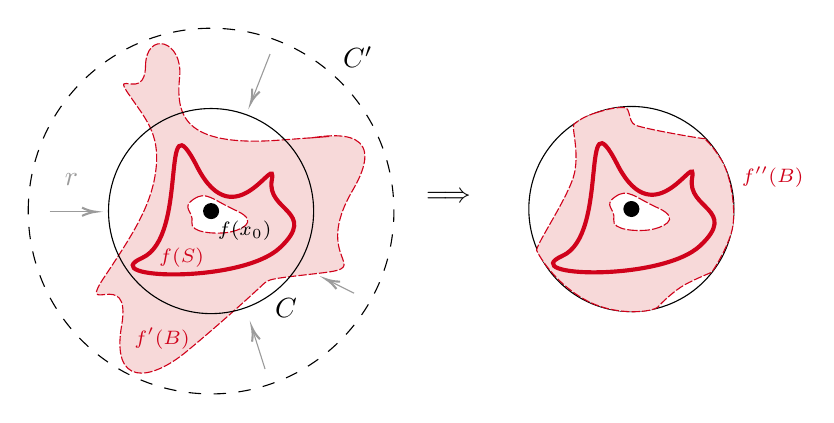
\begin{tikzpicture}[x=0.75pt,y=0.75pt,yscale=-1,xscale=1]
%uncomment if require: \path (0,300); %set diagram left start at 0, and has height of 300

%Shape: Circle [id:dp3818592251235218] 
\draw   (376.75,160.17) .. controls (376.75,132.87) and (398.87,110.75) .. (426.17,110.75) .. controls (453.46,110.75) and (475.58,132.87) .. (475.58,160.17) .. controls (475.58,187.46) and (453.46,209.58) .. (426.17,209.58) .. controls (398.87,209.58) and (376.75,187.46) .. (376.75,160.17) -- cycle ;
%Shape: Polygon Curved [id:ds9912394080956158] 
\draw  [color={rgb, 255:red, 208; green, 2; blue, 27 }  ,draw opacity=1 ][fill={rgb, 255:red, 247; green, 217; blue, 217 }  ,fill opacity=1 ][dash pattern={on 3pt off 0.75pt}] (409.33,113.75) .. controls (416.58,111.5) and (419.08,111.25) .. (422.58,111.25) .. controls (426.08,111.25) and (424.31,118.01) .. (428.08,119.75) .. controls (431.86,121.49) and (461.58,126.66) .. (461.58,126.25) .. controls (461.58,125.84) and (461.33,125.5) .. (461.58,126.25) .. controls (461.83,127) and (463.83,127.75) .. (469.08,135.75) .. controls (474.33,143.75) and (476.33,159.75) .. (475.08,168.25) .. controls (473.83,176.75) and (465.58,190.25) .. (464.58,190.75) .. controls (463.58,191.25) and (454.34,194.9) .. (449.97,197.83) .. controls (445.6,200.76) and (441.33,204.75) .. (439.08,207.25) .. controls (436.83,209.75) and (419.08,212.25) .. (404.08,204) .. controls (389.08,195.75) and (381.58,182.5) .. (380.58,180.25) .. controls (379.58,178) and (396.64,153.45) .. (398.83,142.5) .. controls (401.02,131.55) and (397.08,120.25) .. (398.58,119.25) .. controls (400.08,118.25) and (402.08,116) .. (409.33,113.75) -- cycle ;
%Shape: Polygon Curved [id:ds9813394927604682] 
\draw  [color={rgb, 255:red, 208; green, 2; blue, 27 }  ,draw opacity=1 ][fill={rgb, 255:red, 255; green, 255; blue, 255 }  ,fill opacity=1 ][dash pattern={on 3.75pt off 0.75pt}] (418.42,154.25) .. controls (424.58,150) and (427.17,154.25) .. (439.17,159.75) .. controls (451.17,165.25) and (440.42,169.5) .. (434.67,170.25) .. controls (428.92,171) and (416.67,170.5) .. (417.67,165.25) .. controls (418.67,160) and (412.25,158.5) .. (418.42,154.25) -- cycle ;
%Shape: Polygon Curved [id:ds38745041319497653] 
\draw  [color={rgb, 255:red, 208; green, 2; blue, 27 }  ,draw opacity=1 ][fill={rgb, 255:red, 247; green, 217; blue, 217 }  ,fill opacity=1 ][dash pattern={on 3pt off 0.75pt}] (192.08,91.25) .. controls (192.33,74) and (210.23,78.75) .. (208.52,96.52) .. controls (206.8,114.28) and (209.41,130.48) .. (256.42,127) .. controls (303.43,123.52) and (266.39,126.28) .. (271.06,125.97) .. controls (275.74,125.66) and (311.7,117.43) .. (291.83,151.25) .. controls (271.97,185.07) and (302.41,187.99) .. (277.05,190.96) .. controls (251.69,193.93) and (251.72,193.63) .. (248.42,196.75) .. controls (245.12,199.87) and (230.16,213.61) .. (212.15,228.58) .. controls (194.13,243.54) and (175.51,245.53) .. (180.58,216.25) .. controls (185.65,186.97) and (158.37,213.59) .. (172.54,192.47) .. controls (186.71,171.35) and (195.34,157.55) .. (197.17,140.5) .. controls (199,123.45) and (191.68,116.21) .. (183.73,104.49) .. controls (175.78,92.76) and (191.83,108.5) .. (192.08,91.25) -- cycle ;
%Shape: Polygon Curved [id:ds07955789515918577] 
\draw  [color={rgb, 255:red, 208; green, 2; blue, 27 }  ,draw opacity=1 ][fill={rgb, 255:red, 255; green, 255; blue, 255 }  ,fill opacity=1 ][dash pattern={on 3.75pt off 0.75pt}] (215.17,155.5) .. controls (221.33,151.25) and (223.92,155.5) .. (235.92,161) .. controls (247.92,166.5) and (237.17,170.75) .. (231.42,171.5) .. controls (225.67,172.25) and (213.42,171.75) .. (214.42,166.5) .. controls (215.42,161.25) and (209,159.75) .. (215.17,155.5) -- cycle ;
%Shape: Circle [id:dp508369856855212] 
\draw   (174.25,161.17) .. controls (174.25,133.87) and (196.37,111.75) .. (223.67,111.75) .. controls (250.96,111.75) and (273.08,133.87) .. (273.08,161.17) .. controls (273.08,188.46) and (250.96,210.58) .. (223.67,210.58) .. controls (196.37,210.58) and (174.25,188.46) .. (174.25,161.17) -- cycle ;
%Shape: Circle [id:dp34120181878270195] 
\draw  [dash pattern={on 4.5pt off 4.5pt}] (135.57,161.17) .. controls (135.57,112.51) and (175.01,73.07) .. (223.67,73.07) .. controls (272.32,73.07) and (311.76,112.51) .. (311.76,161.17) .. controls (311.76,209.82) and (272.32,249.26) .. (223.67,249.26) .. controls (175.01,249.26) and (135.57,209.82) .. (135.57,161.17) -- cycle ;
%Shape: Polygon Curved [id:ds28152576362594606] 
\draw  [color={rgb, 255:red, 208; green, 2; blue, 27 }  ,draw opacity=1 ][line width=1.5]  (216.92,139.75) .. controls (235.42,176) and (255.67,131.25) .. (252.92,146.25) .. controls (250.17,161.25) and (275.42,161.25) .. (256.92,178.75) .. controls (238.42,196.25) and (167.42,194) .. (190.42,183.75) .. controls (213.42,173.5) and (198.42,103.5) .. (216.92,139.75) -- cycle ;
%Straight Lines [id:da1736817873350045] 
\draw [color={rgb, 255:red, 0; green, 0; blue, 0 }  ,draw opacity=1 ]   (223.67,161.17) ;
\draw [shift={(223.67,161.17)}, rotate = 0] [color={rgb, 255:red, 0; green, 0; blue, 0 }  ,draw opacity=1 ][fill={rgb, 255:red, 0; green, 0; blue, 0 }  ,fill opacity=1 ][line width=0.75]      (0, 0) circle [x radius= 3.35, y radius= 3.35]   ;
%Shape: Polygon Curved [id:ds06195492653330337] 
\draw  [color={rgb, 255:red, 208; green, 2; blue, 27 }  ,draw opacity=1 ][line width=1.5]  (419.42,138.75) .. controls (437.92,175) and (458.17,130.25) .. (455.42,145.25) .. controls (452.67,160.25) and (477.92,160.25) .. (459.42,177.75) .. controls (440.92,195.25) and (369.92,193) .. (392.92,182.75) .. controls (415.92,172.5) and (400.92,102.5) .. (419.42,138.75) -- cycle ;
%Straight Lines [id:da9417041256513283] 
\draw [color={rgb, 255:red, 0; green, 0; blue, 0 }  ,draw opacity=1 ]   (426.17,160.17) ;
\draw [shift={(426.17,160.17)}, rotate = 0] [color={rgb, 255:red, 0; green, 0; blue, 0 }  ,draw opacity=1 ][fill={rgb, 255:red, 0; green, 0; blue, 0 }  ,fill opacity=1 ][line width=0.75]      (0, 0) circle [x radius= 3.35, y radius= 3.35]   ;
%Straight Lines [id:da25280476934088425] 
\draw [color={rgb, 255:red, 155; green, 155; blue, 155 }  ,draw opacity=1 ]   (252.08,85.5) -- (243.57,107.14) ;
\draw [shift={(242.83,109)}, rotate = 291.49] [color={rgb, 255:red, 155; green, 155; blue, 155 }  ,draw opacity=1 ][line width=0.75]    (6.56,-1.97) .. controls (4.17,-0.84) and (1.99,-0.18) .. (0,0) .. controls (1.99,0.18) and (4.17,0.84) .. (6.56,1.97)   ;
%Straight Lines [id:da9101275960157137] 
\draw [color={rgb, 255:red, 155; green, 155; blue, 155 }  ,draw opacity=1 ]   (249.67,237.25) -- (243.94,219.16) ;
\draw [shift={(243.33,217.25)}, rotate = 72.43] [color={rgb, 255:red, 155; green, 155; blue, 155 }  ,draw opacity=1 ][line width=0.75]    (6.56,-1.97) .. controls (4.17,-0.84) and (1.99,-0.18) .. (0,0) .. controls (1.99,0.18) and (4.17,0.84) .. (6.56,1.97)   ;
%Straight Lines [id:da23225691351404076] 
\draw [color={rgb, 255:red, 155; green, 155; blue, 155 }  ,draw opacity=1 ]   (292.58,200.75) -- (280.87,194.89) ;
\draw [shift={(279.08,194)}, rotate = 26.57] [color={rgb, 255:red, 155; green, 155; blue, 155 }  ,draw opacity=1 ][line width=0.75]    (6.56,-1.97) .. controls (4.17,-0.84) and (1.99,-0.18) .. (0,0) .. controls (1.99,0.18) and (4.17,0.84) .. (6.56,1.97)   ;
%Straight Lines [id:da8805946315305658] 
\draw [color={rgb, 255:red, 155; green, 155; blue, 155 }  ,draw opacity=1 ]   (145.92,161.5) -- (166.08,161.5) ;
\draw [shift={(168.08,161.5)}, rotate = 180] [color={rgb, 255:red, 155; green, 155; blue, 155 }  ,draw opacity=1 ][line width=0.75]    (6.56,-1.97) .. controls (4.17,-0.84) and (1.99,-0.18) .. (0,0) .. controls (1.99,0.18) and (4.17,0.84) .. (6.56,1.97)   ;

% Text Node
\draw (225.67,164.57) node [anchor=north west][inner sep=0.75pt]  [font=\scriptsize,color={rgb, 255:red, 0; green, 0; blue, 0 }  ,opacity=1 ]  {$f( x_{0})$};
% Text Node
\draw (197.42,177.82) node [anchor=north west][inner sep=0.75pt]  [font=\scriptsize,color={rgb, 255:red, 208; green, 2; blue, 27 }  ,opacity=1 ]  {$f( S)$};
% Text Node
\draw (185.42,216.32) node [anchor=north west][inner sep=0.75pt]  [font=\scriptsize,color={rgb, 255:red, 208; green, 2; blue, 27 }  ,opacity=1 ]  {$f'( B)$};
% Text Node
\draw (478.17,138.57) node [anchor=north west][inner sep=0.75pt]  [font=\scriptsize,color={rgb, 255:red, 208; green, 2; blue, 27 }  ,opacity=1 ]  {$f''( B)$};
% Text Node
\draw (326,150.65) node [anchor=north west][inner sep=0.75pt]    {$\Longrightarrow $};
% Text Node
\draw (152,141.65) node [anchor=north west][inner sep=0.75pt]  [color={rgb, 255:red, 155; green, 155; blue, 155 }  ,opacity=1 ]  {$r$};
% Text Node
\draw (286,80.9) node [anchor=north west][inner sep=0.75pt]    {$C'$};
% Text Node
\draw (253.25,202.15) node [anchor=north west][inner sep=0.75pt]    {$C$};


\end{tikzpicture}

    \caption{Proof of Lemma~\ref{lem:bounded-local-mod}.}
    \label{fig:retracting-annulus}
\end{figure}


The following fact is nice to note.

\begin{proposition}\label{prop:stable-surj}
    Suppose $f$ is very stable at $x_0$. Then $f$ is surjective. Moreover, given $x \in X$, if $f'$ is a local modification of $f$ at $x$ then $f'$ is also surjective.
\end{proposition}

\begin{proof}
    Suppose $f$ not surjective. Write $y_0 = f(x_0)$. Fix some $z \in P \setminus f(X)$. It is easy to see that there exists a diffeomorphism $F : P \to P$ such that $F(z) = y_0$, where $F$ acts as the identity outside of a fixed ball $B$ around $y_0$. We can then consider the map $f' := F \circ f$. Since $f$ is regular, we have that $f'$ is a $\delta$-local modification at $x_0$ for some large choice of $\delta > 0$. Note that $y_0 \not \in f'(X)$. In particular, this shows that $f$ is not $\delta$-stable at $x_0$.

    For the second claim, suppose $f''$ is a local modification at $x$ which is not surjective. Then we may apply an identical argument to show that $f$ is not $\delta$-stable at $x_0$ for some large $\delta$. 
\end{proof}

The style of argument in the proof of Proposition~\ref{prop:stable-surj} will be used several times in what is to come, so we encourage the reader to make sure they are comfortable with it.
Observe that this proposition has the following nice consequence.

\begin{proposition}\label{prop:verystableeverywhere}
    Suppose $f$ is very stable at some $x_0 \in X$. Then $f$ is very stable at every $x \in X$.
\end{proposition}
    

\begin{proof}
    If $f$ were not very stable at some $x \in X$, then there is a local modification of $f$ which is not surjective. But then $f$ cannot be very stable by Proposition~\ref{prop:stable-surj}.
\end{proof}

In light of Proposition~\ref{prop:verystableeverywhere}, it makes sense to refer $f$ as simply being \emph{very stable}, with no reference to a particular basepoint.
We now proceed with proving the following theorem, which is the main result of this subsection.


\begin{theorem}\label{thm:stable-map-exists}
    There exists a regular simplicial map $f : X \to P$ which is width-visible and very stable.
\end{theorem}

\begin{proof}
    Fix a regular simplicial map $f : X \to P$ such that $\width(f)$ is minimal amongst all such maps. By Proposition~\ref{prop:rank-visibility-whole-map} we have that that $f$ is $R$-width-visible for some $R > 0$.  We first have the following claim.

    \begin{claim}
        For all $\varepsilon > 0$ there exists a vertex $x \in V(X)$ such that $f$ is $\varepsilon$-stable at $x$. Moreover, we can take each $x$ such that $f(x)$ is special.
    \end{claim}

    \begin{proof}
		Suppose this were not the case for some fixed $\varepsilon > 0$. Choose a maximal $10\varepsilon$-separated subset $S \subset P$. Since $f$ is $1$-Lipschitz, every $y \in f(X)$ is within distance $R$ of a special vertex, so by assuming $\varepsilon > R$ as we may, we can find such $S$ satisfying $S \cap f(X) \subset \mathscr S$.
        
        Using Lemma~\ref{lem:bounded-local-mod} and pasting together all of the local modifications at each $s \in S$ we produce a continuous regular map $f' : X \to P$  such that $f'(X) \cap S = \emptyset$.  In fact, it is easy to see that we may take $f'$ such that $f'(X) \cap B = \emptyset$, where $B = B_P(S;\varepsilon/5)$. However, since $f'$ is continuous and $X$ is simply connected, we may lift $f'$ to a regular map $\widetilde {f'} : X \to \widetilde {P \setminus B}$ to the universal cover. But $\widetilde {P \setminus B}$, which is a geodesic space, is easily seen to be quasi-isometric to a tree by Manning's bottleneck criterion \cite[Thm.~4.6]{manning2005geometry}. However, then $X$ has asymptotic dimension at most 1, which is a contradiction.
    \end{proof}

	Since both $X$ and $P$ are quasi-transitive, we can now translate all these increasingly stable points to one point $x_0$, giving a sequence of maps $f_n$ such that $f_n$ is $n$-stable at $x_0$, and $f_n(x_0) = f_m(x_0)$ for all $n,m \geq 1$. Now, use the Arzel\`a--Ascoli theorem to take a limit $\widehat f$ of the $f_n$. This will satisfy $\width(\widehat f) = \width(f)$, and so since the width of $f$ was chosen to be minimal we again have by Proposition~\ref{prop:rank-visibility-whole-map} that $\widehat f$ is width-visible. 
    We now verify the stability of $\widehat f$.

    \begin{claim}
         $\widehat f$ is very stable.
    \end{claim}

    \begin{proof}
        Write $y_0 = \widehat f(x_0)$. 
        Suppose $\widehat f$ is not $\varepsilon$-stable at $x_0$, for some fixed choice of $\varepsilon > 0$. Without loss of generality, let us assume that $\varepsilon > 10R$. Let $f'$ be a $\varepsilon$-local modification of $\widehat f$ at $x_0$ such that $y_0 \not \in f'(X)$. 
        Choose $n > 0$ such that 
        $$
        f_n|_{B(x_0,\varepsilon)} = \widehat f|_{B(x_0,\varepsilon)}.
        $$
        We also assume that $n$ is chosen to be sufficiently large so that $f_n$ is $\varepsilon$-stable at $x_0$.
        The local modification of $\widehat f$ induces a local modification of $f_n$, say $f'_n$. This also satisfies
        $$
        f_n'|_{B(x_0,\varepsilon)} = \widehat f'|_{B(x_0,\varepsilon)}.
        $$
        We claim that $ y_0 \not \in f'_n(X)$.
		Indeed, suppose there exists $z \in X$ such that $f_n'(z) = y_0$. Either $z \in B_X(x_0,\varepsilon)$ or $z \not \in B_X(x_0,\varepsilon)$. Since $\varepsilon > 2R$ and $\widehat f(x_0)=f_n(x_0)$ is special for $f_n$, the latter cannot happen, so we must have that $z \in B_X(x_0,\varepsilon)$. But in this case, since $f_n'$ and $\widehat f'$ agree on the $\varepsilon$-ball around $x_0$, this also cannot happen. Thus, such a $z$ does not exist, so $ y_0 \not \in f'_n(X)$.
        However, this is a contradiction, as $f_n$ is $\varepsilon$-stable at $x_0$. Thus, it follows that $\widehat f$ is $\varepsilon$-stable at $x_0$, and so since $\varepsilon$ was arbitrary we can conclude that $\widehat f$ is very stable. 
    \end{proof}

    This concludes the proof of the theorem.
\end{proof}


\subsection{Upgrading to a quasi-isometry}\label{sec:upgrade-to-qi}

The third and final step is to show that our width-visible, very stable map $f : X \to P$ is actually secretly a quasi-isometry.

\begin{theorem}
    A regular simplicial map $f:X \to P$ which is width-visible and very stable is a quasi-isometry.
\end{theorem}
\begin{proof}
    Since $f$ is surjective (by Proposition~\ref{prop:stable-surj}), coarsely Lipschitz and $P$ is geodesic, it suffices to show that $f$ is uniformly proper.

    Since $f$ is width-visible, it suffices to check that for all $x,x' \in f^{-1}(\mathscr{S})$, we have that 
    $$
    \dist_P(f(x),f(x')) \geq \rho_-(\dist_X(x,x')),
    $$
    for some $\rho_-(t)\to \infty$ as $t \to \infty$.

    Given $x \in f^{-1}(\mathscr{S})$, and given $T > 0$,
    let $V$ be the connected component of $f^{-1}(B(f(x),T+2R))$ which contains $f^{-1}(f(x))$.
    By regularity, $\diam(V) \leq C(T)$ for some function $C(T)$ independent of $x$.
    Suppose $x' \in f^{-1}(\mathscr{S})$ satisfies $\dist_X(x,x') > C(T)+2R$ but $\dist_P(f(x),f(x')) < T$.  Then $f(x') \notin f|_{B(x,C(T))}$.
    
    Let $F:P \to P$ be a diffeomorphism which is the identity outside $B(f(x),T)$ and inside $B(f(x),T)$ moves $f(x')$ to $f(x)$.
    Then define a local modification $f':X \to P$ of $f$ by $f' = f$ on $X \setminus V$, and $f' = F \circ f$ on $V$.
    Then $f(x) \notin f'(X)$, which contradicts that $f(x)$ is a very stable point of $f$ (Proposition~\ref{prop:verystableeverywhere}).
    Finally, let $\rho_-(t) = \max\{T:C(T)+R \leq t\}$.
\end{proof}


This concludes the proof of Theorem~\ref{thm:upgrading-reg-to-qi}, stated at the start of this section.
We are now ready to finish the proof of our main result, Theorem~\ref{thm:main-result}. The only work left to do is to observe that accessibility allows us to extend beyond the realm of one-ended graphs.

\mainresult*

\begin{proof}
    Let $\Gamma$ be an almost planar, coarsely simply connected, connected, locally finite, quasi-transitive graph. By \cite{hamann2018accessibility}, we have that $\Gamma$ is an accessible graph, as such it can be factorised into a `tree-amalgam' of a  finite collection $\{H_1, \ldots, H_n\}$ of connected, locally finite, quasi-transitive graphs with at most one end (see \cite{hamann2025tree} for definitions).  It is easy to see that these graphs are also almost planar and coarsely simply connected. By Theorems~\ref{thm:intro-hyperbolic-plane} and \ref{thm:upgrading-reg-to-qi}, each of the $H_i$ is either finite or quasi-isometric to either the Euclidean or hyperbolic plane. By \cite{hamann2025tree}, we conclude that $\Gamma$ is quasi-isometric to a free product of free and surface groups, and in particular is quasi-isometric to a planar graph. 
\end{proof}

We will finish this section by providing a direct proof of Corollary~\ref{cor:intro-fpgroups} which does not use the machinery of \cite{macmanus2023accessibility}.

\maincorollary*

\begin{proof}
    Let $G$ be an almost planar, finitely presented group.
    By Dunwoody's accessibility theorem \cite{dunwoody1985accessibility}, $G$ splits as a graph of groups with finite edge groups and finitely presented vertex groups $H_v$ with at most one end. By Theorems~\ref{thm:intro-hyperbolic-plane} and \ref{thm:upgrading-reg-to-qi}, each infinite $H_v$ is quasi-isometric to either the Euclidean plane or the hyperbolic plane. This implies that the vertex groups are all finite or virtual surface groups. Note that virtual surface groups are residually finite and virtually torsion-free.
    It is a classical fact that a group which splits as a graph of groups with finite edge groups and residually finite, virtually torsion-free edge groups is itself residually finite and virtually torsion free. In particular, $G$ has a finite-index subgroup $H$ which splits as a free product of free and surface groups, and so $H$ admits a planar Cayley graph \cite[Thm.~3]{arzhantseva2004cayley}.
\end{proof}


% 
% \section{Proof of Theorem~\ref{thm:fp-subgroups}}
% 
% 
% We now prove Theorem~\ref{thm:fp-subgroups} of the introduction, which is the last result of this paper. 
% 
% 
% 
% \subsection{The flanking lemma}
% 
% 
% In this subsection we prove a helpful result which we dub the \emph{flanking lemma}. The statements in this section are stated for $\mathbb H^2$, as this is sufficient for our purposes. However, much of what follows is also true (with some work) for any generic complete Riemannian plane. 
% First, we need the following. 
% 
% 
% \begin{lemma}\label{lem:component-of-curve}
%     Let $X$ be a connected, simply connected, one-ended,  polygonal complex of bounded geometry. 
%     Let $f : X \to \mathbb H^2$ be a continuous regular map. 
%     Fix $x_0 \in X$. Let $C \subset \mathbb H^2$ be a simple closed curve which separates $f(x_0)$  from infinity. 
% 
%     Then, there exists a connected component $U$ of $C \cap f(X)$ such that for any proper ray $\gamma \subset X$ based at $x_0$, we have that $f(\gamma) \cap U \neq \emptyset$. 
% \end{lemma}
% 
% % Note that $U$ above does not depend on $\gamma$. 
% 
% \begin{proof}
% % [Proof of Lemma~\ref{lem:component-of-curve}]
% Let $Y$ be the space obtained from $\mathbb H^2$ by removing the parts of $C$ that are not covered by $f(X)$, namely $Y = \mathbb H^2 - \left( C - f(X)\right)$. 
% % Given the images of two rays $f(\gamma_1), f(\gamma_2)$ we say that $f(\gamma_1)$ is homotopic relative infinity to $f(\gamma_2)$ if for each $n$ there exists $N > n$ and an homotopy of $\mathring{P}$ that send $f(\gamma_2)$ to $f(\gamma_1)$ in $B_P(x_0, n)$ and to itself outside $B_{\mathring{P}}(x_0, N)$. 
% % 
% % [ Alternative: Let $\tilde{\mathring{P}}$ be the universal cover of $\mathring{P}$.  The map $X \to P$ lifts to $X \to \tilde{\mathring{P}}$ as $X$ is simply connected; let $\tilde{C}$ be the base lift of $C\setminus f(X)$.  If there is no such $U$ then there are two "gates" $U_1, U_2$ in the universal cover and two proper rays $\gamma_1, \gamma_2 \subset X$ from $x_0$ so that their lifts go to an end through $U_1,U_2$ respectively.  $f^{-1}( \mathrm{int}(C))$ then lifts back to a bounded subset of $X$ which disconnects $X$ into at least two ends, containing the ends of $\gamma_1, \gamma_2$ respectively.]
% % 
% % [ (Alternative$)^2$: 
% Let $\widetilde{Y}$ be the universal cover of $Y$.  The map $X \to \mathbb H^2$ lifts to $\widetilde{f} \colon X \to \widetilde{Y}$, as $X$ is simply connected. By Lemma~\ref{lem:one-ended-regular-maps}, we have that $\widetilde{f}(X)$ accumulates in exactly one end.  Let $\widetilde{C}$ be the lift of $C\setminus f(X)$ which separates $\widetilde f(x_0)$ from infinity. Note that each component of $\widetilde{C}$ disconnects $\widetilde{Y}$. In particular, there is only one component of $\widetilde{C}$ that separates the image of $x_0$ from the end on which $\widetilde{f}(X)$ accumulates. This means that the image of every ray $\widetilde{f}(\gamma)$ must intersect such component, yielding the result.
% \end{proof}
% 
% 
% We also introduce the following terminology.
% 
% \begin{definition}[Ray-thick]
%     Let $\Gamma$ be a connected, locally finite graph. We say that $\Gamma$ is \emph{ray-thick} if it satisfies the following additional condition:
%     \begin{equation}\tag{$\Psi$}\label{eq:ray-thick}
%         \parbox{4.5in}{For all $n > 0$ there exists $r > 0$ such that for all $x_0 \in V(\Gamma)$ there exists an end $\omega$ of $\Gamma$ and a collection of $n$ pairwise disjoint combinatorial rays in $\Gamma$ based within $B_X(x_0,r)$, approaching $\omega$.}
%     \end{equation}
%     % If $S = \{X_\alpha\}$ is a collection of complexes, we say that $S$ is \emph{uniformly ray-thick} every $X_\alpha$ is ray-thick with uniform constants.
% \end{definition}
% 
% The existence of a quasi-transitive group action on $\Gamma$ is often enough to ensure that $\Gamma$ is ray-thick.
% 
% \begin{proposition}\label{prop:ray-thick}
%     Let $\Gamma$ be a connected, locally finite,  quasi-transitive, graph. Suppose $\Gamma$ contains a thick end. Then $X$ is ray-thick.
% \end{proposition}
% 
% \begin{proof}
%     Since $X$ has a thick end, it contains infinitely many pairwise disjoint rays approaching this end \cite{thomassen1993vertex}. The quasi-transitivity of the group action now implies property (\ref{eq:ray-thick}). 
% \end{proof}
% 
% % In what follows, we will consider a topological circle that separates a point from infinity. However, it is useful to relax this notion to a homological version. More precisely, let $x$ be a point of a simplicial plane $P$, and let $C$ be an oriented loop so that $C$ represents a non-trivial element of $H_1(P\setminus \{x\})$. Given vertices $z_1, z_2$ of $C$, we say that the ordered pair $(z_1, z_2)$ \emph{doesn't overtake the centre} if for any simplicial geodesic $\gamma$ between $z_2$ and $z_1$ we have that $\gamma + C\vert_{[z_1, z_2]}$ represents the trivial element of $H_1(P\setminus \{x\})$.
% 
% 
% 
% We may now state our key lemma. 
% 
% 
% \begin{lemma}[The flanking lemma]\label{lem:flanking-lemma}
%     Let $X$ be a connected, simply connected, one-ended polygonal 2-complex of bounded geometry, such that the 1-skeleton $X^{(1)}$ is a ray-thick graph.
%     Then for all $\kappa > 0$, $R > 0$,  there exists $D_0 > 0$ such that for all $D > D_0$, $x_0 \in X$, and all continuous $\kappa$-regular maps $f : X \to \mathbb H^2$, there exists $y \in \mathbb H^2$ such that:
%     \begin{enumerate}
%         \item $\dist_{\mathbb H^2}(y,f(x_0)) = D$,
% 
%         \item $B_{\mathbb H^2}(y,R) \subset f(X)$.
%     \end{enumerate}
% \end{lemma}
% 
% % Note that the extra hypothesis on $X$ is easily satisfied by one-ended hyperbolic Cayley complexes. 
% 
% \begin{proof}
%     Fix $D_0$ to be very large, exactly how large we will determine later on.
% 	Let $D > D_0$. Let $C$ be a circle of radius $D$ in $\mathbb H^2$ around $f(x_0)$. Choose a maximal $3R$-separated net $N$ of $C$ with respect to the ambient metric. It is easy to see that the connected components of $C \setminus N$ are uniformly bounded in diameter, bounded by some multiple of $R$. For every $y \in N$, consider the ball $B_y$ of radius $R$ around $y$. If any of the $B_y$ are contained in $f(X)$, we are done. Otherwise, we must have that \emph{every} $B_y$ contains a point which is not in $f(X)$. We now modify $C$ locally in inside each of the $B_y$ so that it passes through these points. Call the new circle $C'$. See Figure~\ref{fig:tambourine} for a cartoon of the construction of $C'$, that satisfyingly resembles a tambourine. 
% 
%     Now, every component of the $C' \cap f(X)$ is uniformly bounded in diameter, where this bound depends only on $R$. However, because $X$ is one-ended and simply connected, we have by Lemma~\ref{lem:component-of-curve} that there exists a component $U \subset C' \cap f(X)$ such that for every ray $\gamma \subset X^{(1)}$ based at $x_0$, we have that $f(\gamma)$ intersects $U$. But, there is an explicit bound on the maximum size of a set of pairwise disjoint such rays in $X^{(1)}$ which could pass through $U$, since it is uniformly bounded in diameter and $f$ is regular. 
%     If we now choose $D_0$ to be large enough so that there are sufficiently many pairwise disjoint rays based in the $D_0/2\kappa$-neighbourhood of any $x \in X$, using the fact that $X^{(1)}$ is ray-thick, then we must get a contradiction. Thus, one of the $B_y$ was contained entirely in $f(X)$. This concludes the proof of the flanking lemma. 
% \end{proof}
% 
% 
% 
% \begin{figure}
%     \centering
%     \input{figures/tambourine}
%     \caption{Constructing the new circle $C'$ in the proof of the flanking lemma. The red paths are not contained in $f(X)$. }
%     \label{fig:tambourine}
% \end{figure}
% 
% 
% % \subsection{Example}
% 
% 
% % We now apply the flanking lemma to show that the following `bad' group is not almost planar.  This does not satisfy any of the previous criteria.
% 
% % \begin{theorem}
% %     The group 
% %     $$
% %     G_0 = \pres{a,b,c,d,e,f}{[a,b]=[c,d]=[e,f]}
% %     $$
% %     is not almost planar.
% % \end{theorem}
% 
% % \begin{proof}
% %     Idea: Iteratively apply the flanking lemma with $X$ taken to be the hyperbolic half-plane to find regions with arbitrarily big preimages. 
% 
% %     Let $X$ be the standard Cayley complex for $G$, triangulated. This is made up of hyperbolic `half planes' glued together in a tree-like way. Let $P$ denote a simplicial plane of bounded geometry. Let $f : X \to P$ be some $\kappa$-regular, simplicial map. Note that if $H \subset X$ is one of the aforementioned half-planes, then the restriction $f |_H : H \to P$ is also a $\kappa$-regular simplicial map.
% 
% %     Fix $N > 1$. We will find a vertex in $P$ with preimage larger than $N$. Since $N$ is arbitrary, this will give a contradiction, and so $f$ cannot be regular and $G_0$ cannot be almost planar. 
% 
% %     Fix $\varepsilon > 0$ such that the $\varepsilon$-neighbourhood of any point in $X$ intersects at least two distinct `branch lines'.
% %     Let $R_0 = 1$. Then, we iteratively define 
% %     $$
% %     R_i = 2D(R_{i-1}, \kappa, P, H) + R_{i-1} + \varepsilon,
% %     $$
% %     for all $1 \leq i \leq N$, where $D( - , \kappa, P, H)$ is as in the flanking lemma~(\ref{lem:flanking-lemma}). 
% 
% %     Fix some initial half-plane $H_{N} \subset X$. By the flanking lemma, let $x_N in H_N$ be such that 
% %     $$
% %     B_P(f(x_N);R_N) \subset f(H_N). 
% %     $$
% %     Then, there exists another half-plane $H_{N-1}$ branching from $H_N$ which lies at distance at most $\varepsilon$ from $x_N$. Let $y_N \in H_{N-1}$ be a nearest point, so 
% %     $$
% %     \dist_X(x_N, y_N) \leq \varepsilon.
% %     $$
% %     Now, using the flanking lemma again, there exists $x_{N-1} \in H_{N-1}$ such that 
% %     \begin{enumerate}
% %         \item $\dist_X(x_{N-1}, y_N) \leq D(R_{N-1})$, and
% 
% %         \item $B_P(f(x_{N-1}), R_{N-1}) \subset f(H_{N-1})$.
% %     \end{enumerate}
% %     Since $f$ is simplicial (and thus 1-Lipschitz), we have that 
% %     $$
% %     \dist_P(f(x_N), f(x_{N-1})) \leq D(R_{N-1}) + \varepsilon.
% %     $$
% %     In particular, we see that 
% %     $$
% %     B_P(f(x_{N-1});R_{N-1}) \subset B_P(f(x_N);R_N).
% %     $$
% %     We now choose $y_{N-1}$ lying in another half-plane $H_{N-2}$, distinct from the previous two half-planes, which lies within $\varepsilon$ of $x_{N-1}$. This is always possible, since the planes branch in a tree-like way, so we will never accidentally pick one of our previous planes. 
% 
% %     Repeating this argument, we find a sequence of half-planes $H_1, \ldots, H_N$ and points $x_i \in H_i$ such that 
% %     $$
% %     B_P(f(x_1);R_1) \subset B_P(f(x_2);R_2) \subset \ldots \subset B_P(f(x_N);R_N),
% %     $$
% %     where $B_P(f(x_{i}), R_{i}) \subset f(H_{i})$.
% %     In particular, $f(x_1)$ is covered by the images of at least $N$ half-planes. Since $N$ was arbitrary, we conclude that $f$ cannot be regular.
% % \end{proof}
% 
% 
% 
% % \newpage
% 
% \subsection{Applying the flanking lemma}\label{sec:flanking-applications}
% 
% We now apply the flanking lemma~(\ref{lem:flanking-lemma}) to prove our last result, Theorem~\ref{thm:fp-subgroups} of the introduction.
% 
% 
% 
% 
% % \subsection{Hyperbolic groups}
% % 
% % First, we study hyperbolic groups via the Gromov boundary.
% % 
% % \begin{theorem}
% % 	\label{thm:non-planar-hyp}
% % 	If $G$ is an infinite hyperbolic group which does not split over finite subgroups as a graph of groups with all one-ended vertex groups virtually Fuchsian, then $G$ is not almost planar.
% % \end{theorem}
% % It suffices to assume $G$ is one-ended and not virtually Fuchsian.
% % Fix a word metric $d$ on $G$ and a visual metric $\rho$ on $\bdry G$ with visual parameter $\epsilon$.
% % 
% % Recall that a metric space $(Z,\rho)$ is \emph{($L$)-linearly connected} if for every $x,y \in Z$, there exists a continuum $J \subseteq Z$ containing $x$ and $y$ and of diameter at most $L \rho(x,y)$.
% % This is also known as the \emph{bounded turning} condition.  Up to increasing $L$ by an arbitrarily small amount, we may assume $J$ is an arc.
% % By a theorem of Bonk--Kleiner, $(\bdry G, \rho)$ is $L$-linearly connected for some $L \geq 1$ we now fix \cite{bonk-kleiner-2005-qhyp-planes}.
% % 
% % A metric space $(Z, \rho)$ is \emph{($N$)-doubling} if for any $x \in Z, r >0$, the ball $B(x,r) \subset Z$ may be covered using at most $N$ balls of radius $r/2$.
% % The boundary $(\bdry G,\rho)$ is $N$-doubling for some $N$ we now fix.
% % 
% % By a theorem of Tukia \cite{tukia1996quasiarcs} (see also \cite{mackay2008quasiarcs}), if $(Z, \rho)$ is an $N$-doubling, $L$-linearly connected complete metric space, then for some $\lambda=\lambda(L,N)$, any two points $x,y \in Z$ may be connected by a \emph{$\lambda$-quasi-arc}, that is, a topological arc which is itself $\lambda$-linearly connected (and doubling, being a subset of a doubling space).
% % A topological arc is quasisymmetric to $[0,1]$ if and only if it is a quasi-arc~\cite{TukiaVaisala-80-qs}.
% % 
% % A subset $A$ of a metric space $(Z,\rho)$ is \emph{($L'$)-uniformly porous} if for every $x \in A$ and $r \in (0, \diam(Z))$, there exists $y \in B(x,r)$ so that $\rho(y,A) \geq r/L'$.
% % \begin{proposition}\label{prop:quasi-arc-porous}
% % 	For $G$, $(\bdry G, \rho)$, $L,N,\lambda$ as above, 
% % 	there exists $L'$ so that any $\lambda$-quasi-arc $A \subset \bdry G$
% % 	is $L'$-uniformly porous.
% % \end{proposition}
% % \begin{proof}%[Proof of proposition]
% %     There is no point $x \in \bdry G$ which has a neighbourhood homeomorphic to an arc, else $G$ would have circle boundary (see, for example, \cite[Thm. 4.4]{kapovich-benakli-2002-boundary-survey}).
% % 
% % 	We now show porosity.
% % 	By self-similarity, it suffices to consider the case that $r \in [r_0,\diam \bdry G]$ for some constant $r_0>0$.
% % 	Suppose the statement fails.  Then there is a sequence of $\lambda$-quasi-arcs $A_i$, points $x_i \in A_i$, radii $r_i \in [r_0, \diam \bdry G]$ so that the neighbourhood $N(A_i, \frac{1}{i})$ contains $B(x_i,r_i)$.
% % 	Choose a subsequence (and relabel) so that $A_i \to A_\infty$ in the Hausdorff distance, $x_i \to x_\infty \in \bdry G$, and $r_i \to r_\infty \in [r_0,\diam \bdry G]$.
% % 	By compactness properties of quasi-arcs, $A_\infty$ is a $\lambda$-quasi-arc.  If $A_\infty$ is a point, the boundary is disconnected, a contradiction.
% % 	If $A_\infty$ is a non-degenerate arc then $x_\infty \in A_\infty$ has a neighbourhood that is a topological arc, contradiction.
% % \end{proof}
% % % By joining $y$ by a $\lambda$-quasi-arc to a nearby point (and enlarging $L'$), we have:
% % % \begin{corollary}
% % % 	For $G$, $(\bdry G, \rho)$, $L,N,\lambda$ as above, 
% % % 	there exists $L'$ so that any $\lambda$-quasi-arc $A \subset \bdry G$
% % % 	and any $x \in A$ and any $\delta < \diam(\bdry G)$,
% % % 	there exists an $\lambda$-quasi-arc $A' \subseteq B(x,\delta)$
% % % 	with diameter $>\delta/L'$ and at distance $> \delta/L'$ from $A$.
% % % \end{corollary}
% % 
% % \begin{proof}[Proof of Theorem~\ref{thm:non-planar-hyp}]
% %     Given a $\lambda$-quasi-arc $A \in \bdry G$, one can construct its convex hull $\Con(A) \subset G$ which is quasi-isometric to a half-space $\bbH^2_+ \subset \bbH^2$ with uniform constants.  Let $H$ and $P$ be simplicial $2$-complexes quasi-isometric to $\bbH^2_+$ and $\bbH^2$ respectively.
% % 
% %     By Theorem~\ref{thm:intro-hyperbolic-plane} $G$ admits a regular map $f:G \to P$, where $P$ is a bounded geometry tiling of $\bbH^2$.
% %     Thus for any $\lambda$-quasi-arc $A\subset G$,
% %     there is a composition $H \to \Con(A) \hookrightarrow G \stackrel{f}{\to}P$ which is a $\kappa$-regular map for uniform $\kappa$.
% % 
% % 	\begin{claim}
% % 		\label{claim:disjoint-convex-hulls}
% % 		There exists $C>0$ so that:
% % 		for any $\lambda$-quasi-arc $A \subset \bdry G$ with $x_A \in \Con(A)$ a closest point to $e \in G$, and any $y \in \Con(A)$ with $d(y,x_A) \geq 10\delta$,
% % 		there exists a $\lambda$-quasi-arc $A' \subset \bdry G$ 
% % 		so that the closest point projection of $\Con(A')$ to $\Con(A)$ is within $C$ of $y$, and $d(\Con(A'),\Con(A)) \in [10\delta, C]$.
% % 	\end{claim}
% % 	\begin{proof}
% % 		Choose $z \in A$ so that $[e,z)$ passes within bounded distance of $y$.
% % 		Let $r = e^{-\epsilon d(e,y)}$, where recall $\epsilon$ is the visual parameter of the visual metric on $\bdry G$.
% % 		By Proposition~\ref{prop:quasi-arc-porous} $A$ is $L'$-uniformly porous, so there exists $z' \in B(z,r)$ with $\rho(z',A) \geq r/L'$.
% % 		
% % 		For $C'\geq 2L'$, connect $z'$ to a nearby point to find a $\lambda$-quasi-arc $A'$ through $z'$ of diameter $r/C' = e^{-\epsilon (d(e,y)+\frac{1}{\epsilon}\log C')}$.  Let $x_{A'}$ be the closest point in $\Con(A')$ to $e$.
% % 		By construction, we have that $d(x_{A'},y) \approx \frac{1}{\epsilon}\log C'$, and $x_{A'},y$ are within bounded distance of the closest point of $\Con(A)$ and $\Con(A')$ in each other.
% % 	\end{proof}
% % 
% %    	Now recall we have a regular map $f:G \to P$, where $P$ is a bounded geometry tiling of $\bbH^2$, so that for any $\lambda$-quasi-arc $A\subset G$,
% %     there is a composition $H \to \Con(A) \hookrightarrow G \stackrel{f}{\to}P$ which is a $\kappa$-regular map for uniform $\kappa$.
% % 	By the flanking Lemma~\ref{lem:flanking-lemma}, then there exists a function $\Phi=\Phi_\kappa$ so that to each radius $R$ there exists $\Phi(R)=D=D_0+1$ so that for each $F: H \to \Con(A) \to P$ $\kappa$-regular as above, there exists $y \in P$ so that $\dist_P(F(o_H),y) = \Phi(R)$ and $B(y, R) \subset F(H)$.
% % 
% % 	Set $R_0 =1$ and inductively define
% % 	$R_n = \kappa C + \Phi(R_{n-1}) + R_{n-1}$.
% % 	Pick $A_0$ a $\lambda$-quasi-arc with diameter $\diam A= \diam \bdry G$.	
% % 	Let $x_0 \in \Con(A_0)$ be a closest point to $e$; $d(e,x_0) \leq C_0$.
% % 	Let $F_0:H \to \Con(A_0) \to P$ be the corresponding $\kappa$-regular map.
% % 
% % 	By the flanking lemma, there exists $y_0 \in P$ at distance $\Phi(R_\kappa)$ from $F(x_0)$ with $B(y_0, R_\kappa) \subset F_0(H)=f(\Con(A_0))$.
% % 	Let $y_0' \in \Con(A_0)$ be a preimage of $y_0$.
% % 	By the Claim, there exists $A_1$ a $\lambda$-quasi-arc with closest point $x_1$ to $e$, and $y_0'$ within $C$ from being the closest point projection of $\Con(A_1)$ to $A_0$.  
% % 	We have $d(f(x_1),y_0) \leq \kappa C$.  
% % 	Let $F_1:H \to \Con(A_1) \to P$ be the corresponding $\kappa$-regular map.
% % 
% % 	By the flanking lemma, there exists $y_1 \in P$ at distance $\Phi(R_{\kappa-1})$ from $f(x_1)$ with $B(y_1, R_{\kappa-1}) \subset F_1(H)=f(\Con(A_1))$.
% % 	But by the choice of $R_\kappa$ we also have $B(y_1, R_{\kappa-1}) \subset B(y_0, R_\kappa)$, so $y_1 \in f(\Con(A_0)) \cap f(\Con(A_1))$.
% % 
% % 	Proceed inductively to find a point $y_\kappa \in \bigcap_{i=0}^\kappa f(\Con(A_i))$.
% % 	Since the convex hulls $\Con(A_i)$ are $10\delta$ separated by construction, we have a contradiction to $f$ being $\kappa$-regular.
% % \end{proof}
% % \todo{John: A bit messy for now, apologies.  I loosely matched notation in 5.2.  Might it make sense for 5.2 to come before 5.1 as it's simpler?}
% % % 
% % % \newpage
% % 
% % \subsection{Infinite-index subgroups}
% 
% % We now apply the flanking lemma to the following intermediate result.
% % Of course, if the surface subgroup conjecture for hyperbolic groups holds, this would imply Theorem~\ref{thm:non-planar-hyp} above.
% 
% \fpsubgroups*
% 
% \begin{proof}
%     Let $H$ be a one-ended, finitely presented subgroup of $G$. By Corollary~\ref{cor:intro-fpgroups}, we may assume without loss of generality that $H$ has infinite-index in $G$, lest $G$ itself be finitely presented.
%     
% 	Consider a generating set for $G$ that contains a generating set for $H$. Let $\Gamma$ be the Cayley graph of $G$ with respect to this generating set. Suppose by contradiction that $G$ was almost planar. By Theorem~\ref{thm:intro-hyperbolic-plane}, either $\Gamma$ is quasi-isometric to the Euclidean plane, or it admits a regular map to the hyperbolic plane. In the first case, we necessarily have that $G$ is virtually $\mathbb{Z}^2$, which does not contain infinite-index, one ended subgroups. Thus, we have that $\Gamma$ admits a regular map into the hyperbolic plane. Let $X$ be obtained from $\Gamma$ by adding the cells corresponding to the relators of $H$. Since $H$ is finitely presented, we can apply Lemma~\ref{lem:cts-extension} to obtain a regular map $f$ from $X$ to $\mathbb{H}^2$. 
%     Our goal is to use the flanking lemma to show that $f$ cannot be $\kappa$--regular for any value of $\kappa$. So, fix $\kappa\in \N$ and let $Y$ be the subcomplex spanned by the vertices of $H$. We have that $Y$ is connected and that $H$ acts  transitively on it. By Proposition~\ref{prop:ray-thick},  $Y$ is ray thick, and the restriction of $f$ to any translate of $Y$ is $\kappa$-regular. Thus, the flanking Lemma (Lemma~\ref{lem:flanking-lemma}) applies to all translates of $Y$ and we find a function $\Phi = \Phi_\kappa$ that to each radius $R$ associates a value $D = D_0 +1$, so that for each translate $gY$ of $Y$ and $x\in gY$ there exist $y\in \mathbb{H}^2$ so that $\dist_{\mathbb{H}^2}(f(x), y) = D$ and $B_{\mathbb{H}^2}(y,R) \subseteq f(gY)$. The idea is repeatedly use the flanking lemma to find $\kappa+1$ different translates of $Y$ so that their images all intersect in $\mathbb{H}^2$, contradicting regularity. 
% 
%     To this end, let $M$ be large enough that for each $x\in X$, the ball of radius $M$ around $x$ intersects at least $\kappa+1$ different translates of $Y$. Such an $M$ exists because $Y$ has infinite index. 
%     Set $R_0 = 1$ and inductively define $R_n = \kappa M + \Phi (R_{n-1}) + R_{n-1}$. 
% 	Let $Y_0 = Y$ and pick any point $x_0\in Y$. By the flanking lemma, there exists a point $y_0\in \mathbb{H}^2$ at distance $\Phi(R_{\kappa})$ from $f(x_0)$ so that $B_{\mathbb{H}^2}(y_0, R_\kappa)$ is contained in $f(Y)$. Consider a preimage $y$ of $y_0$. By the choice of $M$, there is a point $x_1 \in B_X(y,M)$ and a translate $Y_1 \neq Y_0$ of $Y$ that contains $x_1$. Since $f$ is $\kappa$-Lipschitz, we have that $\dist_{\mathbb{H}^2}(f(x_1), y_0)\leq \kappa M$. By the flanking lemma, there is a point $y_1$ at distance $\Phi(R_{\kappa-1})$  from $f(x_1)$ so that $B_{\mathbb{H}^2}(y_1, R_{\kappa-1})\subseteq f(Y_1)$. But by the choice of $R_{\kappa}$ we also have $B_{\mathbb{H}^2}(y_1, R_{\kappa-1}) \subseteq B_{\mathbb{H}^2}(y_0, R_{\kappa})$ and hence $y_1 \in f(Y_0) \cap f(Y_1)$. We proceed inductively by always choosing different translates $Y_i$ and eventually we find a point $y_\kappa \in \bigcap_{i= 0}^\kappa f(Y_i)$. Since the translates of $Y$ are 1-separated, this contradicts the fact that $f$ is $\kappa$--regular. 
% \end{proof}
% 

% \newpage



% \section{Wishlist for a counterexample}

% In this final section, we briefly discuss what is left of Conjecture~\ref{conj:k-planar-conjecture}, with a particular focus on finitely generated groups. Combining all that has come before, we can say with confidence that a  almost planar, one-ended, finitely generated group $G$ is either virtually planar or satisfies the following list of properties:

% \begin{enumerate}
%     \item $G$ is non-amenable.

%     \item $G$ is not finitely presented.

%     \item $\operatorname{sep}_G(n)$ is logarithmic.

%     \item $\operatorname{asdim}(G) \leq 2$.

%     \item Every infinite-index subgroup of $G$ is either finite, virtually free, or not finitely presented.
%     $$
%     \vdots
%     $$
% \end{enumerate}

% To the best of our knowledge, there is no explicit group known which satisfies all of the above. 
% One-ended groups aside, there is still a further problem. There exists infinite-ended, inaccessible groups with no one-ended subgroups. At present, very little is known about the geometry of inaccessible groups, but perhaps a good starting point could be understanding their asymptotic dimension. 


% \bibliographystyle{abbrv}
\bibliography{references}








% \appendix


% \section{Old stuff}




% \subsection{Tree-thick complexes and the flanking lemma}

% We now describe a general framework within which the flanking lemma provides an obstruction to almost planarity. 
% First, some more terminology.


% \begin{definition}[Tree-thick complex]
%     Let $Y$ be a connected, bounded degree, simplicial 2-complex. We say that $Y$ is \emph{tree-thick} if there exists a map $p : Y \to T$ to a bushy tree $T$, and a collection $M \subset V(T)$ of \emph{marked} vertices, such that the following holds:
%     \begin{enumerate}
    
%         \item For every $m \in M$, there exists a collection $S_m$ of subcomplexes of $p^{-1}(m)$ such that $\cup S_m = p^{-1}(m)$, and the collection
%         $$
%         S = \bigcup_m S_m,
%         $$
%         is uniformly ray-thick.

%         \item There exists $C > 0$ such that for any $y \in Y$, there exists $x, z \in Y$ such that
%             \begin{enumerate}
%                 \item we have $x ,z \in B_Y(y,r)$, 
                
%                 \item both $p(x)$ and $p(z)$ are marked vertices, distinct from $p(y)$, and

%                 \item the point $p(y)$ lies on the geodesic between $p(x)$ and $p(z)$. 
%             \end{enumerate}
%     \end{enumerate}
% \end{definition}

% In the above, a \emph{bushy tree} is a simplicial tree where every vertex has degree at least three.
% We now apply the flanking lemma to tree-thick complexes and show that they do not admit regular maps into planes of bounded geometry.

% \begin{lemma}
%     Let $Y$ be a connected, bounded degree, simplicial 2-complex. Suppose $Y$ is tree-thick. Then $Y$ does not admit a regular simplicial map into any simplicial plane of bounded geometry.
% \end{lemma}

% \begin{proof}
%     {\color{red}Standard flanking lemma argument.}
% \end{proof}

% This has the following immediate consequence.

% \begin{theorem}
%     Let $X$ be a Cayley complex of a one-ended, finitely presented group $G$. Suppose $X$ contains a tree-thick subcomplex $Y$. Then $G$ is not almost planar. 
% \end{theorem}

% We now present some applications.


% \begin{corollary}
%     Let $G$ be a one-ended, finitely presented group. Suppose $G$ contains a finitely generated subgroup $K$ which splits non-trivially (we do not exclude the case where $K = G$). Suppose further that $K$ contains a one-ended, finitely presented subgroup $H$ which is elliptic with respect to this splitting of $K$. Then $G$ is not almost planar.
% \end{corollary}

% \begin{corollary}
%     If a one-ended, finitely presented group splits over a two-ended subgroup and is almost planar, then it splits as a graph of virtually free groups with two-ended edge groups. 
% \end{corollary}

% \begin{proof}
%     The vertex groups of the splitting are finitely presented. If they are one-ended we win by the previous result. If not, they are all either virtually free or they contain one-ended subgroups by Dunwoody. We are then once again done by the previous result.
% \end{proof}

% \begin{corollary}
%     The group 
%     $$
%     G_0 = \pres{a,b,c,d,e,f}{[a,b]=[c,d]=[e,f]}
%     $$
%     is not almost planar.
% \end{corollary}

% \begin{proof}
%     It's Cayley complex is clearly tree-thick, since it is an amalgam of a surface group and a free group.
% \end{proof}

% [Groups $G < H$ with infinite image and one-ended finitely presented kernel are not almost planar]

% [2 gen 1 rel groups not almost planar if not surface groups]
% \subsection{CAT(0) groups?}
% Let $G$ be a non-hyperbolic CAT(0) groups, namely a group acting geometrically on a CAT(0) space $X$ that is not hyperbolic. By \cite[Thm.~III.H.15]{bridsonhaefliger:metric}, $X$ contains an isometrically embedded copy of the Euclidean plane $\mathbb{E}^2$. 


% \subsection{Width of pairs}

% Let $X$, $Y$ be topological spaces. We define the \emph{width of $X$ over $Y$} to be
% $$
% \width(X/Y) := \min_{\text{cont. } f : X \to Y} \max_{y \in Y} \#(f^{-1}(y)).
% $$
% Let $T_k$ denote the rooted binary tree of depth $k$. That is, $T_k$ has $2^k$ leaves. The next statement follows from combining \cite[3.1.C]{gromov2010singularities} and \cite{chavez1998cyclic}. 

% \begin{proposition}
%     $\width(T_k /S^1) > k/10$.
% \end{proposition} 

% This bound is not tight as written, but sufficient for our purposes.


% \subsection{Preimages of tracks}

% Let $K$, $L$ be simplicial 2-complexes. Let $f : K \to L$ be a simplicial map. 
% In what follows, by a \emph{track} or \emph{pattern}, we mean in the sense of Dunwoody. 
% The purpose of this section is to describe, given a track $t \subset L$, what $f^{-1}(t)$ looks like in $K$. 
% % By a \emph{partial track} (resp. \emph{partial pattern}), we mean a track (resp. pattern) on some subcomplex of $L$. 


% \begin{proposition}\label{prop:preimage-of-track}
%     Given a track $t \subset L$, we have that $f^{-1}(t)$ is a pattern in $K$. 
% \end{proposition}

% \begin{proof}
    
% \end{proof}

% \subsection{Tracks in cylinders}

% Here, $T_k$ still denotes the rooted binary tree of depth $k$. Let $L$ denote a finite simplicial complex homeomorphic to $T_k \times [0,1]$. We call $L$ a \emph{cylinder}. The subspaces $T_k \times \{0\}$, $T_k \times \{1\}$ are called the \emph{caps} of the cylinder.  A track or pattern $t \subset L$ is said to be \emph{internal} if it is disjoint from the caps. It is called \emph{essential} if it separates the two caps. 

% In this section, we prove the following.

% \begin{proposition}\label{prop:width-of-internal-tracks-in-cylinders}
%     Let $t \subset L$ be an essential, internal track. Let $Y$ be some topological space. Then $\width(t/Y) \geq \width(T_k/Y)$. 
% \end{proposition}



% \begin{proof}
%     We transform $t$ into something homeomorphic to $T_k$ through a finite sequence of moves. Each individual move can only decrease the width over $Y$. 

%     \paragraph{The move:} Let $a\subseteq t$ be so that $a\subseteq e \times [0,1]$ for some $e\in T_k$ and $a$ describes an innermost arc in $t \cap   e \times [0,1]$, that is to say there is a vertex $v\in T_k$ adjacent to $e$ so that $ a \cap v \times [0,1] = \{a^+, a^-\}$ and the restriction of  $v\times [0,1]$ between $a^+, a^-$ does not intersect $t \setminus a$. Let $f_1, f_2$ be the other two edges adjacent to $v$. We modify $t$ by removing an $\epsilon$--neighbourhood of $a$, where the neigbhourhood is with respect to the induced path metric on $t$ and then in each  $f_i \times [0,1]$ we join the two endpoints  of $t\setminus N_\epsilon (a)$ by two segments. Note that  $\vert t' \cap V(T_K)\times [0,1] \vert < \vert t \cap V(T_k) \times [0,1]\vert$.

%     \medskip
    
    
%     As $a$ was innermost, this means that the obtained pattern $t'$ is still essential. Now, suppose that $t'$ is a proper pattern, i.e. it has two connected components. Then there must be a connected component of it that is an essential, internal track. Moreover, since $T_k$ has valence at most $3$, such connected component is homeomorphic to a connected subspace of $t$, we have  $\width(t/Y) \geq \width(t'/Y)$. 
    
%     \textbf{Claim:} 
% \end{proof}


% \subsection{Proving that the bad group is not almost planar}

% We now apply the above to prove the following.

% \begin{theorem}
%     The group $G_0$ is not almost planar.
% \end{theorem}

% \begin{proof}
%     Let $X$ be the usual Cayley complex of $G_0$. Using Proposition~\ref{prop:almost-planar-simplicial-map-char}, let $K$ be a simplicial subdivision of $X$, $P$ a triangulation of the plane, and $f : K \to P$ a simplicial map such that every vertex in $P$ has boundedly many preimages, say at most $N$. 
%     We proceed through a sequence of claims. 

%     \begin{claim}\label{claim:subcx-tree-product}
%         For every $k > 0$ there exists $r = r(k)> 0$ such that for all $R > r$ we have that the annular region 
%         $A_{r,R}(v_0)$ contains a subcomplex $Z$ such that 
%         \begin{enumerate}
%             \item There is a homeomorphism $F : T_k \times [0,1] \to Z$,

%             \item $F(T_k\times \{0\}) \subset S_r(v_0)$ and $F(T_k\times \{1\}) \subset S_R(v_0)$. 
%         \end{enumerate}
%     \end{claim}

%     \begin{proof}
        
%     \end{proof}

%     Now, fix $r = r(30N)$. Let $B_r(v_0)$ denote the ball of radius $r$. Consider $f(B) \subset P$. Let $t \subset P$ be a circular track which encircles $f(B)$. Consider $f^{-1}(t)$. By Proposition~\ref{prop:preimage-of-track}, this is a compact pattern in $K$ which separates $B$ from infinity. Fix $R > r$ such that $f^{-1}(t) \subset B_R(v_0)$.

%     Let $Z \subset A_{r,R}(v_0)$ be as in Claim~\ref{claim:subcx-tree-product}. We have that $t' = f^{-1}(t) \cap Z$ is an internal pattern which separates the two caps of $Z$. Then, there exists a track $s \subset t'$ which is essential. 
%     By Proposition~\ref{prop:width-of-internal-tracks-in-cylinders}, we have that 
%     $$
%     \width(s/S_1) \geq \width(T_{30N}/S^1) > 3N > N. 
%     $$
%     In particular, the restriction $f|_s : s \to t \cong S^1$ maps more than $N$ points onto a single point. This is a contradiction. It follows that $G_0$ is not almost planar. 
% \end{proof}


% \subsection{Alternative argument?}

% In what follows, by a \emph{hyperbolic half-plane} we mean the closure of a connected component of the hyperbolic plane minus a bi-infinite geodesic. By its \emph{boundary line}, we mean the aforementioned geodesic. 

% By a \emph{$\kappa$-regular simplicial map} between simplicial 2-complexes, we mean an abstract simplicial map where vertex preimages have size at most $\kappa$. 
% One would \textbf{hope} the following is true.

% \begin{lemma}\label{lem:surrounded-by-image}
%     Let $H$ denote some fixed uniform triangulation of the hyperbolic plane. Let $x_0 \in H$ Let $P$ denote some bounded-degree 2-dimensional simplicial complex which is homeomorphic to the plane. Let $\kappa > 0$.

%     Then, for all any $r > 0$ there exists $D > 0$ such that for any $\kappa$-regular simplicial map $f : H \to P$, we have that there exists $y \in P$ such that:
%     \begin{enumerate}
%         \item $\dist_P(y, f(x_0)) < D$, and

%         \item $B_P(y,r) \subset f(H)$.
%     \end{enumerate}
% \end{lemma}

% The order of the quantifiers is very important here. In plain english, this says that if we want to be sufficiently `deep' into the image of $H$, we can do so by walking a controlled distance from the image of some (and hence any) point. 

% \begin{proof}[Proof of Lemma~\ref{lem:surrounded-by-image}]
    
% \end{proof}

% It is not too hard to see that this implies that $G_0$ is not almost planar. We can iteratively apply it to find places in $P$ which are covered by arbitrarily many half-planes. 


% % \subsection{Maps into the plane and topological overlap}




% % \begin{lemma}\label{lem:proper-map-into-plane-exists}
% %     There exists a triangulation of the plane $K$ and a continuous regular map $X \to K$ with the property that for every 2-cell $\sigma \subset X$, we have that 
% %     $$
% %     \partial f(\sigma) \subset f(\partial \sigma).
% %     $$
% %     Moreover, $f(\Gamma) \subset K^1$, and the restriction $f|_{\Gamma} : \Gamma \to K^1$ is a regular map of graphs, and is an almost planar drawing of $\Gamma$ in $K$.  
% % \end{lemma}

% % \begin{proof}
% %     By Proposition~\ref{prop:almost-planar-regular-map-char}, there exists a surjective regular map $f : \Gamma \onto \Pi$ where $\Pi$ is a connected, planar, bounded degree graph. Recall the definition of an \emph{almost 2-connected graph} from  \cite[Def.~1.18]{macmanus2023accessibility}
    
% %     \begin{claim}
% %         $\Pi$ is one-ended and almost 2-connected. 
% %     \end{claim}

% %     \begin{proof}
% %         If not, get a pretty quick contradiction to the regularity of $f$.
% %     \end{proof}

% %     Thus, we may assume without loss of generality that $\Pi$ is 2-connected and one -ended. Then, $\Pi$ admits a VAP-free embedding into the plane  \cite[Cor.~1.24]{macmanus2023accessibility}. Using this drawing, we may embed $\Pi$ into a triangulation of the plane $K$ in a standard way, with the $\Pi$ forming a QI-embedded subgraph of the 1-skeleton $K^1$. One can then pass to some barycentric subdivision of $K$ and modify the image of $\Gamma$ a bounded amount so that the image is an almost planar drawing of $\Gamma$. We may now easily extend to a regular map $X \to K$ piecewise linearly to have the desired properties. 
% % \end{proof}


% % \begin{lemma}
% %     Let $f : X \to K$ be as in Lemma~\ref{lem:proper-map-into-plane-exists}. Then there exists $m > 0$ such that for all $p \in K$ we have that $f^{-1} (p)$ intersects at most $m$ cells.
% %     % \todo{If cells don't inject, this isn't quite true as written. There exists singular points with infinite pre-image coming from a bounded number of cells. } 
% % \end{lemma}

% % \begin{proof}
% %     % Suppose not, so there exists a sequence of points $p_n \in K$ such that 
% %     % $
% %     % |f^{-1} (p_n) 
% %     % $
% %     % Fix $\kappa > 0$ such that the restriction $f|_{\Gamma} : \Gamma \to K^1$ is a $\kappa$-regular map of graphs. In particular, preimages of this restriction have cardinality at most $\kappa$. Thus, at least $n-\kappa$ points in $|f^{-1} (p_n) |$ lie in the interiors of 2-cells. Let $\sigma_1, \ldots, s$
% % \end{proof}



% \newpage

% \subsection{Skeleton of the proof}

% Let $\Gamma$ denote the Cayley graph of $G_0$ corresponding to the above presentation. 
% Let $X$ be the corresponding Cayley complex with 1-skeleton $X^1 = \Gamma$. We may metrise $X$ so that it is a CAT(-1) space. 




% \begin{lemma}\label{lem:spheres_that_folds_too_much}Let $B$ be the horrible sphere with spheres. Then every continuous \textcolor{blue}{surjective?} map from $B$ to $S^1$ needs to have points with large preimage.\end{lemma}
% \begin{proof}
% TO DO, also, to figure out the precise statement.
% \end{proof}

% Let $X$ be the universal cover of three one-boundary tori attached along the boundary. We can metrise $X$ so that it is a CAT(-1) space. 


% \begin{proposition}\label{prop:large_preimages_of_points}
%     For every continuous map from $\phi \colon X\to \mathbb{R}^2$, there is a sequence of points $a_n \in \mathbb{R}^2$ so that $\vert \phi^{-1}(a_n)\vert \geq n$.
% \end{proposition}
% \begin{proof}
%     Let $B$ be a ball inside $X$, let $o$ be its center and for simplicity assume that $\partial B$ does not intersect any branch line. Since $B$ is connected and compact, $\phi(B)$ is a connected and bounded set in $\mathbb{R}^2$. In particular, there exists a circle $C$ so that $\phi(B)$ is in the interior of $C$. 
%     \textcolor{blue}{We would like $C\subseteq \phi(X)$. I believe that the best way to do this is the following: maybe require that $\phi$ is proper, consider a sequence $B_n$ of nested balls in $X$ that contain $B$, and argue that there must be $N>>0$ so that $\dist_{\mathrm{Haus}}(\phi(B), \phi(B_n))>0$, otherwise we would have a contradiction (work out). This should allow to find a topological circle $C$ that contains $B$ and is contained in $\phi(X)$} By the blue part, $C$ is in $\phi(S)$. 
    
%     Look at $\phi^{-1}(S)$. This is a set that separates $X$ into at least two components, one which contains $B$. \textcolor{blue}{Since $\phi$ is proper}, the connected component that contains $B$ is bounded, hence there is a ball $B'$ also centered at $o$ that contains $\phi^{-1}(C)$. Let $S = \partial B$ and $S'= \partial B'$. 
    
%     \textbf{Claim} Let $Y \cong \partial B \times [0,1]$. Then there is an embedding $\iota \colon Y \hookrightarrow X$ so that $\iota(\partial B \times \{0\})  =S$, $\iota(\partial B\times \{1\} \subseteq S'$ and $C$ separates  $\iota(Y)$. 

%     \medskip

%     \textit{Proof of claim}
%     Let $r, r'$ be the radii of $S, S'$ respectively and denote by $S_t$ the sphere of radius $t$ centered at $0$. Let $t_0<t_1\in [r, r']$ be two smallest radi so that $S_{t_0}$ intersects a (finite set of) branch lines that $S_r$ did not intersect and $S_{t_1}$ intersects a new set of branch lines. For $t\in [r, t_0]$ define $Y_r = S_r$. At time $t_0$, for each newly intersected branch line $L_i$, let $Z_{L_i}$ be a connected component of $X\setminus L$ that does not contain $o$, and define $T_t$ for $t\in (t_0, t_1]$ as the ball of radius $t$ in $X\setminus \cup Z_{L_i}$. By repeating this process we define $Y_t$ for all $t\in [r, r']$, and the desired homeomorphism is given by radial coordinates. 

%     \medskip
    
    
%     \textcolor{blue}{Then there must be an embedding of $Y =B \times [0,1] \hookrightarrow X$ so that $B\times {0} = B$, the latter as the subspace of $X$, and $B\times {1}\subseteq B'$. As $C$ separates $Y$ and does not intersect its boundary, some topology should tell you that there is a subspace $D \subseteq\phi^{-1}(C)$ so that $D \cong B$.} By the blue part, there is a continuos map from $B$ to $C \cong S^1$ \textcolor{blue}{that is surjective since $C \subseteq \phi(X)$}. By Lemma~\ref{lem:spheres_that_folds_too_much}, we get a contradiction.
% \end{proof}

% \begin{theorem}
%     Let $\Gamma$ be the Cayley graph of our group with respect to sensible generators.  Then $\Gamma$ is not $k$--planar for any $k$.
% \end{theorem}
% \begin{proof}
%     By putting the appropriate CW structure on the space $X$, we can assume that $\Gamma= X^{(1)}$, and that all 2-cells are  pentagons. Assume by contradiction that $\Gamma$ was $k$--planar for some $k$. \textcolor{blue}{This induces a (continuous, proper, piecewise-linear..) map from $X$ to $\mathbb{R}^2$} so that there is a sequence of points $a_n$ with large preimage. By definition of $k$--planarity, if a point in $\mathbb{R}^2$ is in the image of $\Gamma = X^{(1)}$, then it is the image of a single vertex, or of most $k$ points contained in edges. Thus, for $n$ sufficiently large we can assume that most preimages of $a_n$ are contained in the interior of 2-cells $D_i$. For each $D_i$, note that $\phi(\partial D_i)$ can intersect at most $5k$ images of boundaries of other cells, so by taking $n$ very large, we can find a subsequence of 2-cells $D_{i_s}$ so that $\phi(\partial D_{i_s}) \cap \phi (\partial D_{i_t}) =\emptyset$ whenever $s \neq t$. \textcolor{blue}{Since we can assume that the image of edges is injective, there should be potentially subsets of faces whose images are topological circles that contain at least a vertex that are nested into each other, and wlog $\partial B_{i_s}$ is nested into $\partial B_{i_t}$ if $s\leq t$. By having $n$ very large, we can assume that there is a very long sequence of nesting starting from $\partial B_{i_1}$ then going to $\partial B_{i_s}$ and finally to a family of $5k+1$ elements $\{\partial B_{i_{t_1}},\dots \partial B_{i_{t_{5k+1}}}\}$. In $X$, find paths from $B_{i_1}$ to each element of  $\{\partial B_{i_{t_1}},\dots \partial B_{i_{t_{5k+1}}}\}$ that are as disjoint as possible, namely that have as little common prefix as possible. By insuring that $h$ is large enough, we are ensuring to make progress on the prefix, so that each of the paths must be disjoint when intersecting $\partial B_{i_h}$. But those are now too many paths}.
% \end{proof}



% \section{QI-Embeddings of the Bad Group}

% In this section we try to prove the following theorem. 

% \begin{theorem}
%     Let $G$ be a one-ended, non-virtually Fuchsian, hyperbolic group. Then there exists a QI-embedding $\Gamma_0 \to G$. 
% \end{theorem}

% This, together with a proof that $\Gamma_0$ is not almost planar, would imply the main conjecture for all hyperbolic groups.

% Strategy outline:

% \begin{enumerate}
%     \item Case of no local cut points: Build a quasisymmetric embedding $\partial_\infty G_0 \to \partial_\infty G$.

%      $\partial_\infty G$ is annularly linearly connected.  It contains a quasi-circle.  Use the methods of [Mackay 2014] to unzip the quasi-circle inductively into a linearly connected subspace homeomorphic to $\partial_\infty G_0$.  Use the formalization from [Bonk--Meyer 2022 "Uniformly branching trees"] to get a quasi-symmetry.

%     \item Cast of local cut points: Consider Bowditch's JSJ decomposition of $G$ with tree $T$, and the JSJ decomposition of $G_0$ with tree $T_0$.  Want to build a map $T_0 \to T$ which extends to a QI embedding $G_0 \to G$.  Build vertex by vertex in $T$.  For a quadratically hanging vertex almost by definition have a QI between the vertex spaces.  The tricky case is a rigid vertex, where you want to build a quasi-circle through a sequence of jumps, and again use [Bonk--Meyer] to match up with $G_0$...
% \end{enumerate}







% % Given such a map $f : T_k \to I$ as above,  define the \emph{stacking number} of $f$ as
% % $$
% % {\rm stack}(f) = \sup_{z\in I} |f^{-1}(z)|.
% % $$
% % We call such a map $f$ \emph{optimal} if it minimises the stacking number for the given $k$. 
% % For simplicity, we assume that any given $f : T_k \to I$ restricts to an injection on the leaves of $T_k$. 
% % Consider a standard drawing of $T_k$. From left-to-right, label the leaves $l_1, \ldots, l_K$, where $K = 2^k$. Every map $f : T_k \to I$ induces a total order on the set of leaves. In other words, it induces a permutation of the set $[K] := \{1,\ldots,K\}$. 

% % Note that any $g \in \Aut(T_k)$ also induces a permutation of the set $[K]$, and so we have an embedding $\Aut(T_k) \to S_K$. A permutation in $S_K$ which lies in the image of this map shall be called \emph{automorphic}. 
% % Call a map $f : T_k \to I$ \emph{good} if the permutation it induces on $[K]$ is automorphic. 








\end{document}
